\documentclass[12pt,notitlepage]{report}
\usepackage{amsmath,amsfonts,amssymb,amsthm,amscd,booktabs,comment,euscript}
\usepackage{float,graphicx,mathtools,paralist,makeidx,nameref,aliascnt,tocloft}
\usepackage[usenames,dvipsnames]{xcolor}
\usepackage[all,cmtip]{xy}
\usepackage{amssymb}
\usepackage{latexsym}
\usepackage{proof}
\usepackage{graphicx}
\usepackage{ebproof}
\usepackage{tikzsymbols}
\def\Overrightarrow#1{\mathrlap{\overrightarrow{\phantom{#1\mkern11mu}}}%
  \overrightarrow{#1}}
  


\makeindex
%\usepackage{diagrams}
%\usepackage[all]{xy}
\usepackage{UOMScthesis_Wei}
\usepackage[colorlinks=true, pdfstartview=FitV, linkcolor=blue, citecolor=blue, urlcolor=blue, breaklinks=true]{hyperref}

%Margin Settings
%\leftmargin=0in
%\topmargin=0pt
%\headheight=0pt
%\oddsidemargin=0in
%\evensidemargin=0in
%\textheight=8.75in
%\textwidth=6.5in
%\parindent=0.5cm
%\headsep=0.2in
%\widowpenalty=1000

%Italicised Theorems
\theoremstyle{plain}
\newtheorem{theo}{Theorem}[section]
\newtheorem{nontheo}[theo]{Non-theorem}
\newtheorem*{theo*}{Theorem}
\newtheorem{prop}[theo]{Proposition}
\newtheorem{nprop}[theo]{Non-Proposition}
\newtheorem{lem}[theo]{Lemma}
\newtheorem{cor}[theo]{Corollary}
\newtheorem{claim}[theo]{Claim}
\newtheorem{conj}[theo]{Conjecture}

%Roman Script Theorems
\theoremstyle{definition}
\newtheorem{defin}[theo]{Definition}
\newtheorem{definprop}[theo]{Definition/Proposition}
\newtheorem*{rem*}{Remark}
\newtheorem{rem}[theo]{Remark}
\newtheorem{rems}[theo]{Remarks}
\newtheorem{example}[theo]{Example}
\newtheorem{examples}[theo]{Examples}

%Math Operators
\DeclareMathOperator{\id}{id}
\DeclareMathOperator{\im}{im}
\DeclareMathOperator{\cod}{cod}
\DeclareMathOperator{\dom}{dom}
\DeclareMathOperator{\hset}{Hom}
\DeclareMathOperator{\Ob}{Ob}
\DeclareMathOperator{\Or}{o}
\DeclareMathOperator{\Ar}{Mor}
\DeclareMathOperator{\coker}{coker}
\DeclareMathOperator{\fr}{Rank}
\DeclareMathOperator{\subob}{Subob}
\DeclareMathOperator{\gr}{gr}
\DeclareMathOperator{\SA}{SA}
\DeclareMathOperator{\supp}{supp}
\DeclareMathOperator{\Aut}{Aut}
\DeclareMathOperator{\Oh}{O}
\DeclareMathOperator{\typ}{typ}
\DeclareMathOperator{\Typ}{Typ}
\DeclareMathOperator{\Int}{Int}
\DeclareMathOperator{\Inv}{Inv}
\DeclareMathOperator{\Ped}{Ped}


%New commands
\newcommand\FS{\mathbf{Free_1}}
\newcommand\fs{\mathbf{F}}
\newcommand\far{\mathrm{Farey}}
\newcommand\A{\mathcal{A}}
\newcommand\B{\mathcal{B}}
\newcommand\Cb{\mathcal{C}}
\newcommand\E{\mathcal{E}}
\newcommand\C{\mathbb{C}}
\newcommand\HQ{\mathbb{H}}
\newcommand\Z{\mathbb{Z}}
\newcommand\Q{\mathbb{Q}}
\newcommand\R{\mathbb{R}}
\newcommand\LX{\mathbf{LX}}
\newcommand\N{\mathbb{N}}
\newcommand\K{\mathbb{K}}
\newcommand\PS{\mathcal{P}}
\newcommand\Ef{\mathcal{E}}
\newcommand\Yu{\mathbf{U_{mon}}}
\newcommand\Ell{\mathcal{L}}
\newcommand\Are{\mathcal{R}}
\newcommand\G[1]{G_0(#1)}
\newcommand\SG[1]{G_0(#1,\tplus)}
\newcommand\GI[1]{G^{\mathrm{iso}}(#1)}
\newcommand\SI[1]{S^{\mathrm{iso}}(#1)}
\newcommand\NI[1]{N_0(#1)}
\newcommand\SN[1]{N_{\tplus}(#1)}
\newcommand{\arxiv}[1]{\href{http://arxiv.org/abs/#1}{\tt arXiv:\nolinkurl{#1}}}
\newcommand\tplus{\>\widetilde{\oplus}\>}
\newcommand\ttimes{\>\widetilde{\otimes}\>}
\newcommand\tminus{\>\widetilde{\ominus}\>}
\newcommand\Tplus{\widetilde\oplus}
\newcommand\Ttimes{\widetilde\otimes}
\newcommand\Tminus{\widetilde\ominus}
\newcommand\wplus{\>\widehat{\oplus}\>}
\newcommand\Wplus{\widehat{\oplus}}
\newcommand\bplus{\>\bar{\oplus}\>}
\newcommand\Bplus{\bar{\oplus}}
\newcommand\dee{\mathbf{d}}
\newcommand\are{\mathbf{r}}
\newcommand\aye{\mathbf{a}}
\newcommand\bee{\mathbf{b}}
\newcommand\cee{\mathbf{c}}
\newcommand\gp{\sim^{gp}_\mu}
\newcommand\gpd{\sim^{gpd}_\mu}
\newcommand\gpc{\simeq^{gp}_\mu}
\newcommand\BO{B_\Omega^\oplus}
\newcommand\RO{R_\Omega^\oplus}
\newcommand\MO{M_\Omega^\oplus}
\newcommand\MN{M_n^\oplus}
\newcommand\ef{\mathbf{f}}
\newcommand\you{\mathbf{u}}
\newcommand\ifc{\Eye(\N)_\mathbf{fc}}



\newcommand\zero{\mathbf{0}}
\newcommand\one{\mathbf{1}}
\newcommand\two{\mathbf{2}}
\newcommand\three{\mathbf{3}}
\newcommand\dd{\downdownarrows}
\newcommand\op{\mathrm{op}}


\newcommand\cat{\mathbf{C}}
\newcommand\catar{{\cat^{\rightarrow}}}
\newcommand\xat{\mathbf{X}}
\newcommand\gcat{G_0(\mathbf{C})}
\newcommand\catt{\mathbf{D}}
\newcommand\cattt{\mathbf{E}}
\newcommand\adcat{\mathbf{A}}
\newcommand\adcatt{\mathbf{A}'}
\newcommand\meow{\mathbf{Cat}}
\newcommand\univ{\mathcal{U}}
\newcommand\gen{\mathrm{GL}_n}
\newcommand\pow{\mathcal{P}}
\newcommand\set{\mathbf{Set}}
\newcommand\grp{\mathbf{Grp}}
\newcommand\MVEA{\mathbf{MVEA}}
\newcommand\ab{\mathbf{Ab}}
\newcommand\fab{\mathbf{FinAb}}
\newcommand\fgab{\mathbf{Ab}^{\mathrm{fg}}}
\newcommand\mon{\mathbf{Mon}}
\newcommand\rng{\mathbf{Ring}}
\newcommand\crng{\mathbf{CRing}}
\newcommand\vect[1]{\mathbf{Vect_\mathbb{#1}}} %These commands now have an argument for the field, the argument must be percisely a capital letter
\newcommand\fvect[1]{\mathbf{FinVect_\mathbb{#1}}}
\newcommand\rel{\mathbf{Rel}}
\newcommand\fset{\mathbf{FinSet}}
\newcommand\rmod[1]{#1\text{-}\mathbf{Mod}}
\newcommand\prmod[1]{#1\text{-}\mathbf{pMod}}
\newcommand\cmod{\C\text{-}\mathbf{Mod}}
\newcommand\sub{\mathbf{Sub}}
\newcommand{\define}[1]{\emph{#1}\index{#1}}
\newcommand\BA{\mathbf{BA}}
\newcommand\EA{\mathbf{EA}}
\newcommand\MV{\mathbf{MV}}
\newcommand\BCM{\mathbf{BCM}}
\newcommand\GLU{\mathbf{Grp_{LU}}}
\newcommand\Gi{\mathcal{G}}
\newcommand\Jay{\mathcal{J}}
\newcommand\Dee{\mathcal{D}}
\newcommand\Em{\mathcal{M}}
\newcommand\Pee{\mathcal{P}a}
\newcommand\Tee{\mathcal{T}\!o}
\newcommand\catj{\mathbf{J}}
\newcommand\Eye{\mathcal{I}}

\newcommand{\eqstar}{\mathop{*}\limits}

\newcommand\sprod{{\scriptstyle \, \prod \,}}
\newcommand\scoprod{{\scriptstyle \, \coprod \, }}
\newcommand\tprod{{\scriptscriptstyle \, \prod \,}}
\newcommand\tcoprod{{\scriptscriptstyle \, \coprod \, }}

% Diagram Macros
\newcommand{\diagprod}[9]{& #4 \ar@{.>}[d]_{#9} \ar[dl]_{#7} \ar[dr]^{#8} &  \\
                                            #2   & #1 \ar[l]_{#5} \ar[r]^{#6}   & #3 }
\newcommand{\diagcoprod}[9]{& #4  &  \\
     #2 \ar[r]^{#5} \ar[ur]^{#7}  &  #1 \ar@{.>}[u]^{#9}  & #3 \ar[l]_{#6} \ar[ul]_{#8}}
     


\numberwithin{equation}{section}


\newcommand*{\toccontents}{\@starttoc{toc}}



\begin{document}

\numberwithin{figure}{chapter}

\title{Formally verified code obfuscation in the Coq Proof Assistant}
\author{Weiyun Lu}
\copyrightfalse
   \tablespagefalse
\beforepreface
\pagenumbering{gobble}
\setcounter{chapter}{0}

\thispagestyle{empty}




\chapter*{Abstract}
\renewcommand{\thepage}{\roman{page}}
\setcounter{page}{2}
\renewcommand*\theenumi{\alph{enumi}}
\renewcommand*\labelenumi{(\theenumi)}
\addcontentsline{toc}{chapter}{Preliminaries}
\addcontentsline{toc}{section}{Abstract}
Code obfuscation is a software security technique where transformations are applied to source and/or machine code to make them more difficult to analyze and understand to deter reverse-engineering and tampering.  However, in many commercial tools, such as Irdeto's \emph{Cloakware} product, it is not clear why the end user should believe that the programs that come out the other end are still the ``same program"!
\par In this thesis, we apply techniques of formal specification and verification, by using the Coq Proof Assistant and IMP (a simple imperative language within it), to formulate what it means for a program's semantics to be preserved by an obfuscating transformation, and give formal machine-checked proofs that these properties hold.
\par We describe our work on opaque predicate and control flow flattening transformations.  Along the way, we also employ Hoare logic as an alternative to state equivalence, as well as augment the IMP program with Switch statements.  We also define a lower-level flowchart language to wrap around IMP for modelling certain flattening transformations, treating blocks of codes as objects in their own right.
\par We then discuss related work in the literature on formal verification of data obfuscation and layout obfuscation transformations in IMP, and conclude by discussing CompCert, a formally verified C compiler in Coq, along with work that has been done on obfuscation there, and muse on the possibility of implementing formal methods in the next generation of  real-world obfuscation tools.

\chapter*{Acknowledgements}
\addcontentsline{toc}{section}{Acknowledgements}
I would like to thank my advisors, Prof. Amy Felty and Prof. Philip Scott,  for their direction throughout this journey.  I thank my supervisor at Irdeto, Bahman Sistany, for introducing me to the area of code obfuscation.  
\par Thanks to Prof. Guy-Vincent Jourdan, Prof. Luigi Logrippo, and Prof. Liam Peyton for serving on my thesis committee.
\par Gratitude to my parents and grandparents for nurturing in me an insatiable desire to learn new things from a young age.
\par Finally, thank you to OGS and the University of Ottawa for the generous funding.



\newpage


\tableofcontents

\chapter{Introduction to obfuscation}\label{intro}

We set the stage for this thesis by introducing the concept of \define{obfuscation} of code, give a motivating example using realistic languages and tools in the real world, and discuss the benefits and indeed, need, for applying tools of formal verification to this field of software security.

\renewcommand{\thepage}{\arabic{page}}
\setcounter{page}{1}
\renewcommand*\theenumi{\alph{enumi}}
\renewcommand*\labelenumi{(\theenumi)}

\section{Obfuscation in the wild}
Obfuscation \cite{CoNa} is a security technique whereby source or machine code is deliberately changed, with the intention of concealing its true purpose, so that it is more difficult for a human or a tool to read, analyze, and understand.  This can be done either by manually changing code, or by applying algorithmic transformations --- our interest will primarily be in the latter.
\par Reasons for a software developer to wish to do such a thing include deterring and/or preventing the tampering of software or its reverse engineering.  For example, a Pay TV box which has the cryptographic keys securing it physically inside the device given to the end consumer needs to be obfuscated so that it cannot easily be hacked by a tech-savvy user.  On the other hand, obfuscation can also used by the Bad Guys\texttrademark to hide (by obfuscating signatures that these tools would otherwise pick up on) the presence of malware or viruses from scanning tools.
\par In practice, many of the finer details of obfuscation as it is used in the real world are, at best, vague.  For instance, the actual increased difficulty of reverse engineering a program is difficult to measure.  Also, one needs some reasonable certainty that the transformed program still ``behaves the same way" as the original program.  This is often poorly defined, and consequently difficult to actually \emph{prove}.  This is important and interesting not only from an academic point of view, but also when selling obfuscating software to potential clients.
\par \define{Irdeto}, the cybersecurity company where the present research began as a co-op term, creates a product called \define{Cloakware Software Protection} \cite{CSP} which, among other things, protects software by applying many layers of varying obfuscating transformations on code.  Two of the most common questions asked by prospective clients during presentations of this product are
\begin{itemize}
    \item What is the tradeoff in performance versus security?
    \item How do I know my program still functions as intended after going through these transformations?
\end{itemize}
The first question can be partially answered, in that certain bounds for how much larger or slower the files become in relation to the level of security desired can be given.  The second, however, needs to be handled with indirection and danced around, because in fact, there \emph{is no} formal specification or guarantee of correctness, and one simply has to \emph{believe} that Irdeto knows what they are doing in this regard.  As an academic with a background in mathematical logic and theorem proving, such a response is \emph{highly} unsatisfactory!

\par The subject of this thesis is to study individual obfuscating transformations in a modular way, formalizing their definitions in the \emph{Coq proof assistant} \cite{Coq}, formalizing various ways of expressing that the transformed code is semantically equivalent to the original code, and then proving these assertions indeed hold.


\subsection*{A note on explanation of proofs}\label{proofexplain}
In the first sample proof in Section \ref{demorgansec}, we will walk the reader through a Coq proof and explain every step, providing screenshots of the updated proof state at every line.
\par In the remaining proofs of the thesis, while everything is completely worked out in Coq, with screenshots attached and also available in source code at \cite{repo}, we will not explain every single step in the text where it does not add anything meaningful to the understanding of what is going on.
\par Often, some parts of the proofs are mechanical and are indeed quite analogous or similar to previously explained steps in the same proof or a previous proof, and there is not much value in going over the same motions again.
\par Rather, the approach will be to explain enough to give the reader a high-level account of the process, and in particular discuss any new tactics or ideas that have not been seen before.  In other words, we provide \emph{all} the detail of the proof in the code and the screenshots, but will aim to \emph{explain in text} enough to get the point across, rather than get bogged down in the unnecessary monotony (for both the author and the reader) of each and every step.

\section{Motivating example: reverse engineering a simple C program}\label{motivating}\index{reverse engineering}

Before we continue with the formalisms in Coq, we present the reader with a small motivating example of realistic languages and tools.  \define{Radare2} \cite{R2} is a tool for reverse-engineering C binaries, and one application is to solve \define{Crackme}\footnote{See, for instance, \href{https://crackmes.one/}{https://crackmes.one/}.} challenges - that is, a binary with a hidden password that when executed, will prompt the user to input it.  Solving it yields a congratulatory message whereas entering an incorrect password results in an (often sarcastic) error message.

\par One of the obfuscating transformations that we study in this thesis is the use of \define{opaque predicates}, which we will introduce early for the purposes of this example.

\subsection{Opaque predicate obfuscation}

\begin{defin}[Opaque predicate]\label{opaquedefn}
	An \define{opaque predicate} \cite{CoNa} is a predicate\footnote{This could be any statement in a program that could evaluate to true or false, but we will only be concerned with arithmetic formulas in this thesis.  Our use of the word ``predicate" is more general than that in predicate logic \cite{vanDalen}.} that evaluates to either \emph{true} or \emph{false} 100\% of the time (that is, regardless of the specific values of any of the variables) and the truth-value of which is known to the programmer writing the code, but is nevertheless evaluated at runtime.
\end{defin}

Of course, the absolutely most basic opaque predicates are just the boolean constants \emph{true} and \emph{false} themselves, but these are not very useful in practice because it is immediately obvious what is happening in the program, and neither the simplest of humans nor tools will be fooled.  

\par We thus need a minimum baseline of non-obviousness (note that this property is not technically part of the standard definition) to achieve any amount of increased security.  Many SMT\footnote{``SMT" stands for ``satisfiability modulo theory"; see for example \href{https://en.wikipedia.org/wiki/Satisfiability_modulo_theories}{https://en.wikipedia.org/wiki/Satisfiability\_modulo\_theories}.  These implement decision problems in various theories in first-order logic and are widely used in verification, correctness, software testing, etc.  A treatment is also in \cite{HuRy}.} solvers\index{SMT solver}, such as those packaged into the tool SMTCoq \cite{SMTCoq} (and indeed, Coq's built-in \emph{omega} tactic) can automatically analyze universally quantified equations over linear integer arithmetic\footnote{Statements in predicate logic with universal quantifiers (for all) over arithmetic equations involving integers of degree at most 1 (no quadratics or higher).}, but cannot handle higher-order polynomials.

\begin{example}
	An opaque predicate presented\footnote{Strictly speaking, the predicate is just the $[(x * x) + x]\mod 2 = 0$ part, but, for convenience and as an abuse of notation/terminology, we will refer to the sentence containing the quantifier $\forall x \in \N$ as the opaque predicate.  That is, in the practical examples throughout this thesis, we use and refer to universally quantified equations as opaque predicates.} in \cite{Opaque} is
    \[
    	\forall x\in\N.\ [(x * x) + x]\mod 2 = 0.
    \]
    After a moment's reflection, we realize this is a tautology, though it is not immediately obvious at first glance.
\end{example}

\begin{example}
    Another interesting example, and a way to achieve \define{diversity} (that is, different versions of the same program after it has been obfuscated), is with a \define{parametrized opaque predicate}.  For instance, fixing any particular $D \in \N$, we obtain an opaque predicate
    \[
        \forall x,y,z\in\N.\ ( D \neq 0 \land D = z^2) \Rightarrow x^2 - Dy^2 \neq 1.
    \]
\end{example}

\begin{example}\label{running_ex}
	Our running example for opaque predicate obfuscation will be even simpler, as the simple language inside Coq that we will use does not have modular arithmetic built in, and we wish to focus on the obfuscation technique itself without getting bogged down in details.  We use the simpler (but still out of reach of linear solvers) opaque predicate
    \begin{equation}\label{runningex}
    	\forall x\in\N.\ (x * x + x + x + 1) = (x + 1) * (x + 1).
    \end{equation}
\end{example}

Our opaque transformation then works as follows.  If the original program is $c_1$ and we let $c_2$ be an arbitrary program, and $P(x)$ is our opaque predicate, then the transformed program looks like\footnote{This is the notation in Coq that is used to express if-then-else statements in imperative programs.  The ``B" in ``IFB" refers to the fact that the guard condition is a boolean.  We will see details later about how such programs are formally defined in Coq.}

\begin{verbatim}
    IFB (P x) THEN c1 ELSE c2 FI.
\end{verbatim}

The idea is that \emph{we} know that $P(x)$ will always be true and so c1 will always execute and c2 never will, but that a person or tool applying static analysis to the code will not immediately realize this fact.


\par Using our example predicate, we show the difference between solving a simple Crackme with and without the obfuscating transformation.  Let us be slightly dramatic, and suppose that the user is actually attempting to defuse a bomb --- and thus only has one shot to guess the correct password.  Furthermore, the bomb has a timer of, say, five minutes, and will automatically detonate if not successfully defused in the allotted time.
\subsection{The unobfuscated program}

Consider the C source code below for the main function of the unobfuscated bomb program.  We start with $x=3$, reassign $x = x + x$, and compare this to the user input, and hence the password that needs to be entered is simply 6.

\begin{verbatim}
int main(int argc, char **argv) {
    int x, y;
    x = 3;
    x = x + x;

    printf("Enter the code to defuse the bomb: ");
    scanf("%d", &y);

    if (y == x) {
        printf("Correct code.  Bomb defused.\n");
        return 0;
    } else {
        printf("Wrong code.  Boom.\n");
        return -1;
    }
}
\end{verbatim}

Below is the visual mode of Radare2 analyzing the compiled binary.  It is not important for the reader to understand the exact details of all of these low level instructions (as this is simply a motivating example with a real-world tool, but \emph{not} the main point of the thesis), but to simply keep in mind the difference in the general visual structure of the control flow between Figures \ref{fig:radare2} and \ref{fig:radare2}.

\begin{figure}[H]
    \centering
    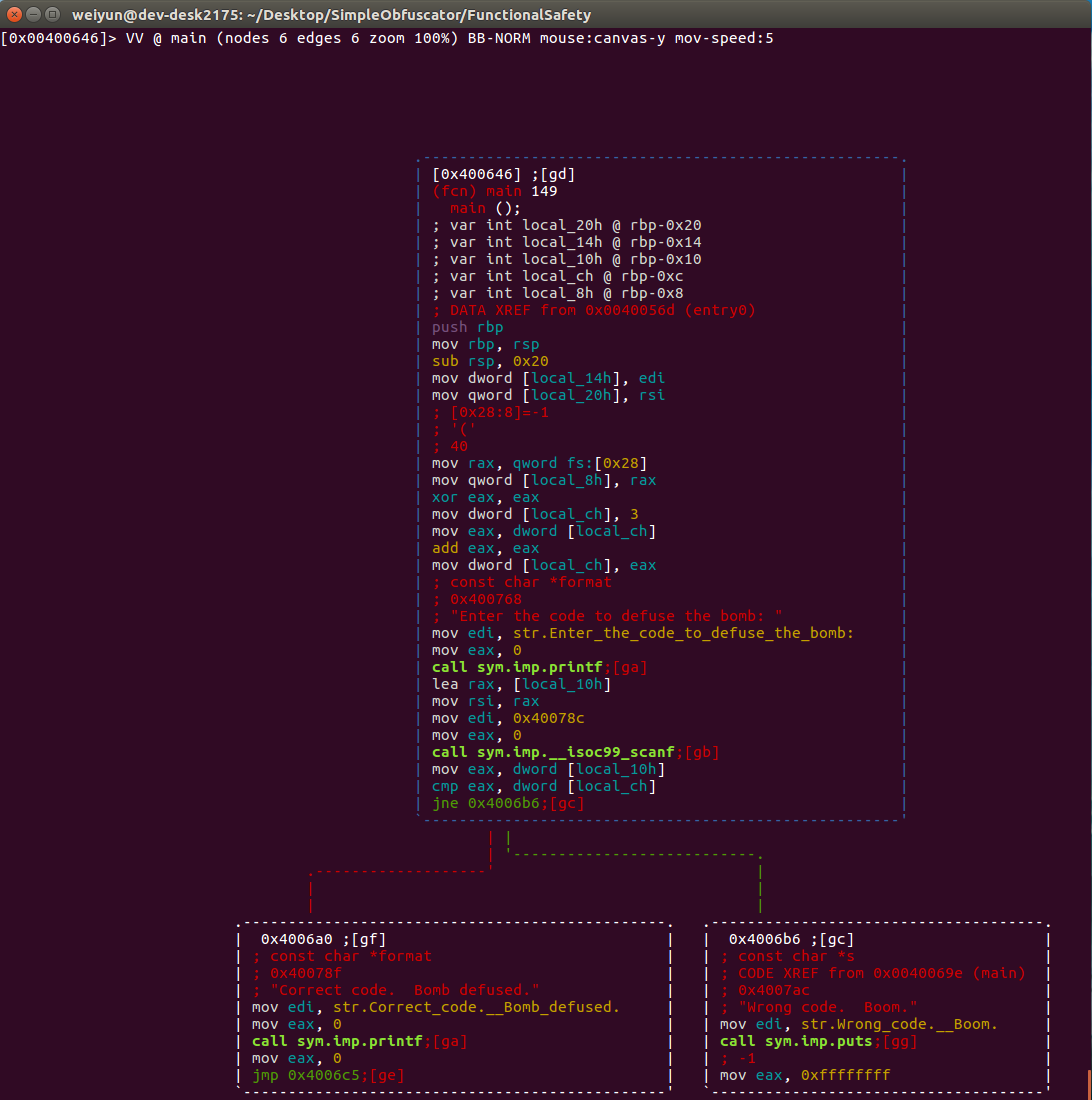
\includegraphics[scale=0.42]{r2simple}
    \caption{Radare2, unobfuscated program}
    \label{fig:radare}
\end{figure}

We can recover, from the shape of the control flow in Figure \ref{fig:radare}, that there is a branch in the program, and the presence of the string ``Bomb\_defused" tells us the left branch is what we want.  We see, on the final few lines in the top block before the branching, that there is a $cmp$ (comparison) instruction between two variables $eax$ and $dword [local\_ch]$.

\par Now, with the Radare2 user assumed to know that $mov$ corresponds to assignment and $lea$ corresponds to reading input, we can fairly quickly trace the flow from bottom up and recover that one of these values must be $3+3$ and the other value is the user input, and so the password must be 6.  For even a beginner user of Radare2, this analysis is not difficult and could easily be solved in under 5 minutes.

\subsection{The obfuscated program}

Now let's obfuscate the program with our opaque predicate \eqref{runningex}.  In fact, to make the program even more confusing to analyze, we'll let the user supply the value for opaque predicate computation (introduced as the variable $z$), under the guise of ``the first code'', whereas the real password we ask for is the ``second code''.  
\par Of course, the predicate is always true, so $x = 3 + 3 = 6$ is still always the second code that will diffuse the bomb independent of what value is entered as the first code.

\begin{verbatim}
int main(int argc, char **argv) {
    int x, y, z;

    x = 3;

    printf("Enter the first code to defuse the bomb: ");
    scanf("%d", &z);

    if (z * z + z + z + 1 == (z + 1) * (z + 1)) {
        x = x + x;
    } else {
        x = x * x;
    }

    printf("Enter the second code to defuse the bomb: ");
    scanf("%d", &y);

    if (y == x) {
        printf("Correct code(s).  Bomb defused.\n");
        return 0;
    } else {
        printf("Wrong code(s).  Boom.\n");
        return -1;
    }
}
\end{verbatim}

Again, we analyze the compiled binary in Radare2's visual mode.  We again stress that the important thing here is the overall control flow in comparison with Figure \ref{fig:radare}, and not the details of all the individual low-level instructions.

\begin{figure}[H]
    \centering
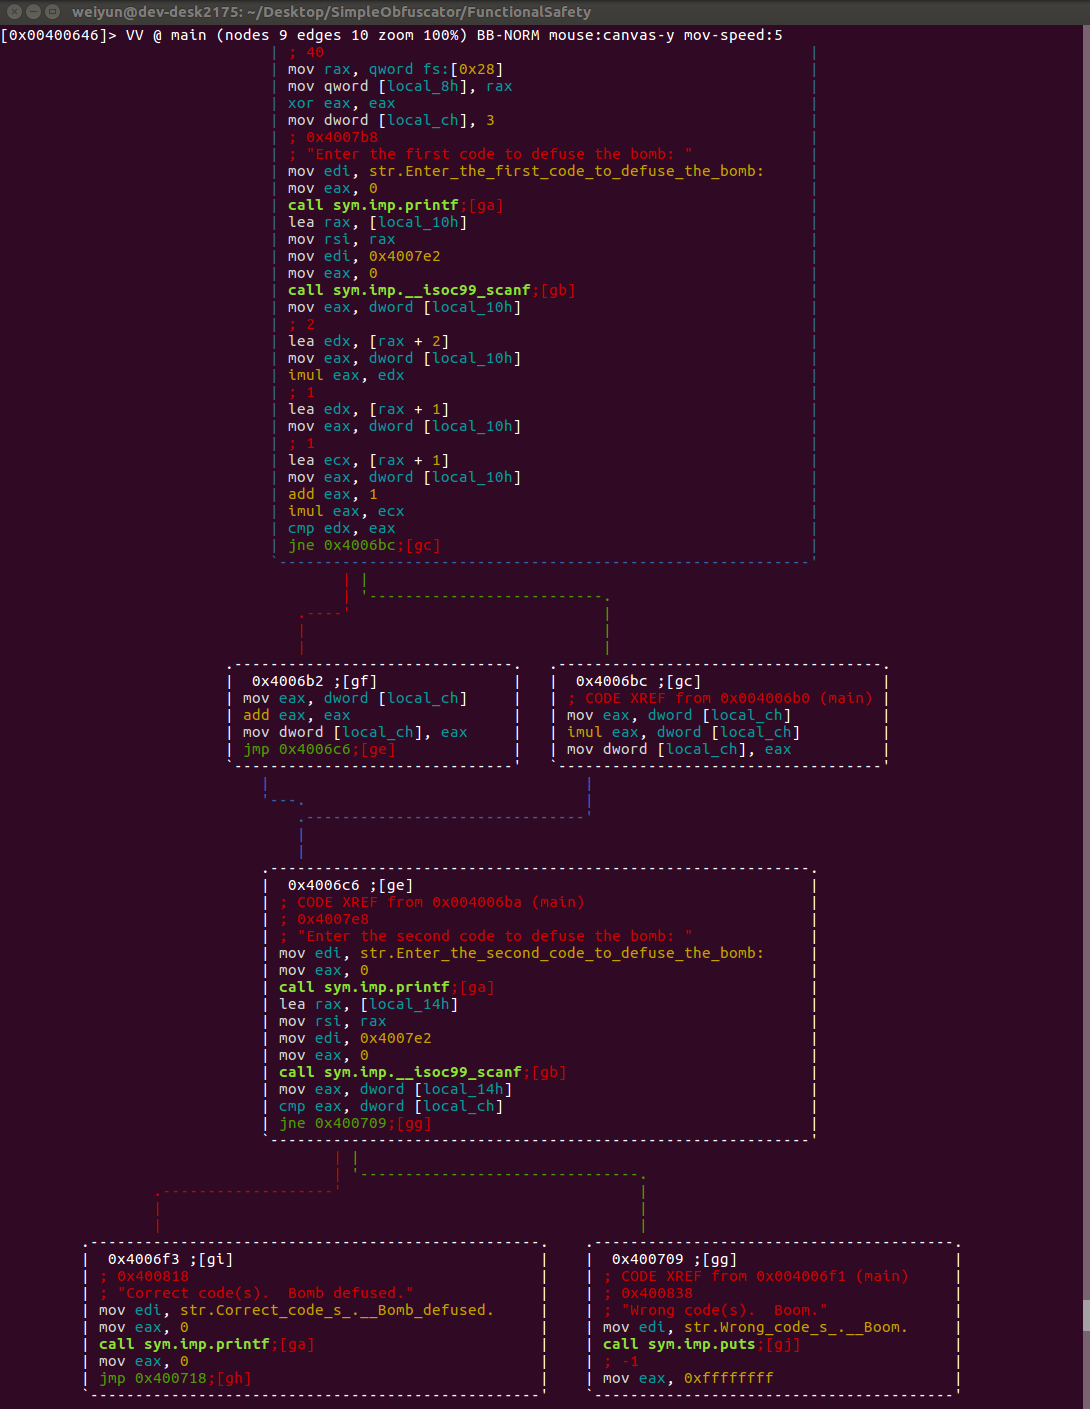
\includegraphics[scale=0.4]{r2obfuscated}
    \caption{Radare2, obfuscated program}
    \label{fig:radare2}
\end{figure}

Things are looking a little more complicated now in Figure \ref{fig:radare2}.  If one starts at the bottom and traces upwards from the second $cmp$ command right before the final branch, and travels through both of the branches resulting from the first $cmp$, one can recover that the second code must be either $6$ or $9$.

\par What is not obvious at this point, however, is \emph{which} of the two it is, and moreover, the fact that the first code actually has no impact on the answer.  Note that there are a number of additional commands before the first $cmp$ statement that correspond to the low-level assignments that are made to do the opaque predicate evaluation.  \par Certainly, if a Radare2 user sits down for a few extra minutes and thinks it through, it will eventually become apparent what's really going on, but this requires more work.  And remember --- we're dealing with a ticking bomb and we don't \emph{have} a few extra minutes.  We may have to just bet all our chips on a gamble --- input any value for the first code, and input either 6 or 9 for the second code moments before the bomb goes off, and hope for the best!  We will revisit this idea formally in Section \ref{weakened}.

\par As contrived as this example may seem, it is actually a good metaphor for the goals of obfuscation in the real world.  Take the \define{Denuvo}\footnote{See \href{https://www.denuvo.com}{https://www.denuvo.com.}} digital rights management\index{DRM} solution for video games (acquired recently by Irdeto), for example --- game developers use this product to protect their games knowing full well that it is overwhelmingly likely that their product will eventually be cracked (that is, someone is able to bypass the anti-piracy check and run an illegally obtained copy of the program) in spite of their best efforts.  But given that the majority of a new hit video game's sales are in the first few weeks after it is released, then simply by delaying the emergence of a crack, the obfuscation has done its job.

\par Where formal verification comes into play now is to prove that the obfuscating transformation preserves key properties of interest.  In the case of our bomb example, we'd better be sure that the intended defuse code will still work.  In the case of Denuvo and games, perhaps we want to prove some bounds on the effect that the DRM has on performance.

\section{Summary of contributions}

The obfuscation algorithms studied in this thesis are well-known, but the novelty of our work is in our approach of formalizing them in the Coq proof assistant and proving them correct.  In particular:

\begin{itemize}
    \item We bring together the perspectives of computer science, pure mathematics, and logic, and offer an explanation from an interdisciplinary viewpoint of how formal verification is useful and, indeed, has been used already in major real-world projects.
    \item We consider different formulations of what it means for a transformation to be semantics-preserving, including complete state equivalence as well as Hoare logic equivalence.  In this particular setting, the latter is a novel approach, and we give examples of its use with opaque predicate transformations.
    \item We give clear and detailed explanations of the proofs and tactics in Coq, which, to the best of our knowledge, the existing literature does not, thus providing an accessible explanation of not just obfuscation techniques, but also in tandem with its formalization and verification inside Coq.
    \item We begin with a minimal imperative programming language inside Coq for reasoning about programs and their transformations, and then augment it as needed for control flow flattening algorithms, first by augmenting its syntax and semantics with switch statements, and then by defining a lower-level flowchart language that wraps around blocks of code in order to model real-world intermediate languages used in obfuscation tools.
    \item We obtain and explain insights on how formal verification allows us to ``catch bugs before they even make it into the code", and demonstrate how we sometimes need to come up with additional assumptions to make our statement correct, and how this can abort what could otherwise have been catastrophes in production code --- in particular, in coming up with invariants that imply a  variable introduced by a transformation did not exist in the original program.

\end{itemize}

\chapter{Background --- formal verification}\label{two}
In this chapter we provide necessary background information used for formal verification --- namely, the Coq proof assistant, the simple imperative language IMP defined inside Coq, and Hoare logic for reasoning about pre- and post-conditions of programs.
\section{The Coq proof assistant}

Coq \cite{Coq} is a formal proof management system, an implementation of the \define{Calculus of (co)inductive constructions}, which provides a formal language in which one can write mathematical definitions, algorithms and theorems, and an environment for the development of machine-checked proofs.  It is implemented (mostly) in OCaml\footnote{See \href{https://www.ocaml.org}{https://www.ocaml.org}.} and (a little bit of) C.
\par The development of Coq began in 1984 at \define{INRIA} (\emph{Institut national de recherche en informatique et en automatique}) in France, now also in collaboration with the \'{E}cole Polytechnique, Universit\'{e} Paris-Diderot, and Universit\'{e} Paris-Sud.  Now developed by a team of more than 40 people, it was initiated by G\'{e}rard Huet and Thierry Coquand.  
\par Coquand's name is one explanation given for why Coq is named as it is. Another is the claim to a local tradition of naming French research development tools after farm animals \cite{CoqFaq} (as ``coq" means ``rooster" in French).  Finally, there is the explanation that it derives from a shortening of ``Calculus of Constructions" where the final C is replaced by a Q for some reason.  To the present author, the numerosity of explanations makes the whole thing seem a bit of a surreal stretch, but that is neither here nor there and we will leave the discussion of the name at that.
\par Code written in Coq is remniscent of functional languages like Scheme or Lisp, with the addendum of \define{proof states} whenever we enter the proof of a theorem.  As long as one trusts Coq's kernel, and one believes the statement of a theorem (or proposition, or example\footnote{Coq has keywords \emph{Theorem}, \emph{Proposition}, \emph{Example}, \emph{Lemma}, all of which are to make a statement that the user has to prove.  They all serve the same function, but it is just a matter of style for the user to choose one.  For instance, a property of a function applied to a specific example could be an Example in Coq, whereas general significant theorem could be a Theorem in Coq.  Even a statement made as an Example needs to be proven correct to be valid.} --- these are all just different labels for the same thing to Coq) is correctly specified, then the fact that one is able to execute a Coq script past the save point of the theorem means that it can be trusted to be correctly proven or verified, without the need to pore over every detail.  
\par This is in stark contrast to, say, mathematical theorems proven on paper, which often have gaps in reasoning (or just as dubiously, pointing the reader to another resource which itself may not give a full argument, or simply ``leaving it as an easy exercise") that require either a much larger effort or leap of faith on the reader's part, or to traditional testing of software\footnote{In traditional testing of software, a test case is typically an \emph{example} that some specific inputs give a desired result, as opposed to a \emph{theorem} that can be about entire classes of inputs with the expressive power of predicate logic.}, which cannot possibly cover all the relevant cases or offer absolute assurance that the thing will do what it says on the box.  
\par We give a whirlwind tour of some high-level projects that have used formal verification, and Coq specifically, to demonstrate its proven track record of applicability and usefulness in industrial software development, and then explain proof states and tactics in Coq as they relate to the work of this thesis.


\subsection{Coq in the wild}

\subsubsection{CompCert certified C compiler}
Something formally defined and proven in Coq leads to a high assurance of correctness --- one example of this is \define{CompCert} \cite{CompCert} by Xavier Leroy's\index{Xavier Leroy} team, a formally verified compiler written in Coq for (a large subset) of C.  The upshot of CompCert being formally verified is that it will not cause \emph{miscompilation errors} --- that is, the executable code produced is proven to behave exactly as the semantics specified by the source program.
\par At the time of this writing, CompCert is already over 120000 lines of code.  It can be freely downloaded for research and educational purposes, or a license can be purchased for commercial use.  It has been shown to be no worse than twice as slow as its contemporaries such as GCC\index{GCC} --- not that bad of a tradeoff for compatible projects that require the additional assurance!

\subsubsection{Formalizing mathematics}
\par Formalizing mathematics is an idea that dates back to David Hilbert's\index{David Hilbert} program in the early part of the twentieth century.  The advent of modern computer proof assistants such as Coq has caused a resurgence in this field, as we see in the following theorems.
\par Coq allows for partial automation of repetitive cases, making feasible proofs that would otherwise not be, due to a large numbers of cases that need to be manually checked, such as the proof of the \define{Four-Colour Theorem} from graph theory, which states the following.
\begin{theo}[Four-colour Theorem]
Given any separation of a plane into contiguous regions (called a \emph{map}), no more than four colours are required to colour the regions of the map so that no two adjacent regions have the same colour.
\end{theo}
Originally conjectured in 1852, it remained an open problem for over a century.  A first seemingly complete proof with computer assistance (but not in a formal theorem prover) appeared in \cite{Appel}, but this required trust in the unverified programs used by the authors.  Finally, it was formally proven correct in 2005 using Coq by Georges Gonthier's\index{Georges Gonthier} team at Microsoft \cite{Gonthier}.

\par Another monumental proof completed formally by Gonthier's team is the \define{Feit-Thompson Theorem} \cite{Gonthier2} from algebraic group theory.  This did have an existing analogous paper proof, but it is so long and requires so many intermediary theorems and lemmas that many mathematicians were not fully convinced of its correctness.  We give the statement of the theorem below, but as the present thesis is in computer science and not pure mathematics, we will not explain what all of the terms mean and instead refer the interested reader to \cite{DF} as a starting point.

\begin{theo}[Feit-Thompson Theorem]
    Every finite group of odd order is solvable.
\end{theo}

\par A major project that reimagines the foundations of mathematics as type-theoretic rather than set-theoretic (together with the \define{univalence axiom}, which stipulates that equality itself is equivalent to equivalence), \define{Homotopy Type Theory}, or HoTT for short, also bears mentioning.  The HoTT book \cite{HoTT} was first written entirely in Coq, then only later deformalized into a print book for human reading --- the opposite direction of how things usually go in this business!  This project was endowed with a 7-figure grant from the United States Department of Defense\index{Department of Defense}.

\subsubsection{Preventing catastrophes}
\par Finally, we offer the reader some cautionary tales of what can happen in the \emph{absence} of formal verification, and how it has become adopted in the aftermath.

\par The failure of the Ariane 5 rocket \cite{Ariane}\index{Ariane 5 rocket} launch caused a 7 billion dollar project to crash and burn (literally) because of a single line of code --- an erroneous type casting of a 64-bit float to a 16-bit integer representing the rocket's tilt that resulted in onboard computers entering emergency shutdown.  This is a bug that would not have escaped rigorous formal verification, the use of which has since become standard practice in such mission-critical systems.

\par More recently, the world of cryptocurrencies and blockchains has seen some projects adopting formal verification for \define{smart contracts}.  The \define{Ethereum} \cite{Ethereum} blockchain, which is the first blockchain to introduce smart contracts, runs on its own scripting language called \emph{Solidity} based loosely on JavaScript.  A high-profile attack on a vulnerability allowed attackers to drain what at the time was worth 64 million USD and resulted in the chain being hard-forked\footnote{This means the blockchain split into two versions.  In the original Ethereum chain, the attack was rolled back.  But in the forked chain, called Ethereum Classic, the effects of the attack remain, following the tenet of ``code is law".}.  
\par Two newer blockchain projects that aim to offer more secure smart contracts by way of supporting formal verification (among other improvements that are beyond the scope of the present discussion) are \define{Tezos} \cite{Tezos} and \define{Cardano} \cite{Cardano}, whose respective smart contract languages \define{Michelson} and \define{Plutus} are based on OCaml.  They are also among the first scientific blockchains, employing teams of PhDs, producing peer-reviewed research papers, and forging partnerships with universities.
\par While these projects are still young and have much to prove in the way of real world use and adoption, they already command respectable value in the cryptospace --- at the time of this writing both are in the top 20 coins by market capitalization --- a strong indication of investor interest and that the future of smart contracts moving large amounts of value through blockchains may indeed be one in which formal verification plays a critical role\footnote{Note that formal verification cannot, and is not meant to, prevent losses due to keys and passwords being misplaced or stolen.  Rather, it is to verify that the code that governs a smart contract is indeed correct and will behave as specified.}.

\subsection{Detailed sample proof: DeMorgan's Theorem}\label{demorgansec}
We now explain how proving a theorem in Coq works by way of detailed example; we will prove (one of) \define{DeMorgan's theorem}(s).  We will assume the reader is familiar with the basics of propositional and predicate logic, constructive (intuitionist) logic, and proofs by natural deduction.  An excellent resource for background is \cite{vanDalen}.
\par For the purpose of elucidation, for this proof, we will walk through every single line and explain the changes to the proof state and goals with some screenshots along the way.  For the remaining proofs throughout the thesis, we will, for the sake of both our and the reader's sanity, be less verbose than this.  The full Coq code for the entire thesis is available in the accompanying GitHub repository \cite{repo}, and the interested reader is welcome to set up Coq and execute them if he or she wishes to see the play-by-play in action.

\begin{theo}[DeMorgan's Theorem]\label{DeMorgan}
    For all propositions $P, Q$,
    \[
        \neg (P \lor Q) \Longleftrightarrow \neg P \land \neg Q.
    \]
    \begin{proof} The syntax to declare this theorem in Coq is
    \begin{verbatim}Theorem deMorgan : forall P Q : Prop, ~(P \/ Q) <-> ~P /\ ~Q.\end{verbatim}
        The proof goal is now the statement of the theorem itself.  The first tactic we apply is 
        \texttt{intros Po Qo}, which \emph{instantiates} the propositions P and Q.  This is equivalent to saying, in natural language, ``let $P_0$ and $Q_0$ be arbitrary propositions".  In Figure \ref{fig:demorgan1st}, we see the Coq IDE after applying this; the window in the top-right shows the current proof state.  Above the line, we have $P_0, Q_0 : Prop$, which tells us that this is a current hypothesis, whilst below the line the proof goal has changed to 
        \[
        \neg (P_0 \lor Q_0) \Longleftrightarrow \neg P_0 \land \neg Q_0. \]
        That is, the goal is now to prove the equation holds for this particular $P_0$ and $Q_0$ that we have instantiated.  In Figure \ref{fig:demorgan1st}, we see in the upper-right window the proof state after executing the latest command.  We continue showing the figures for each step throughout this example.
        \par \medskip \noindent
\begin{figure}[H]
    \centering
          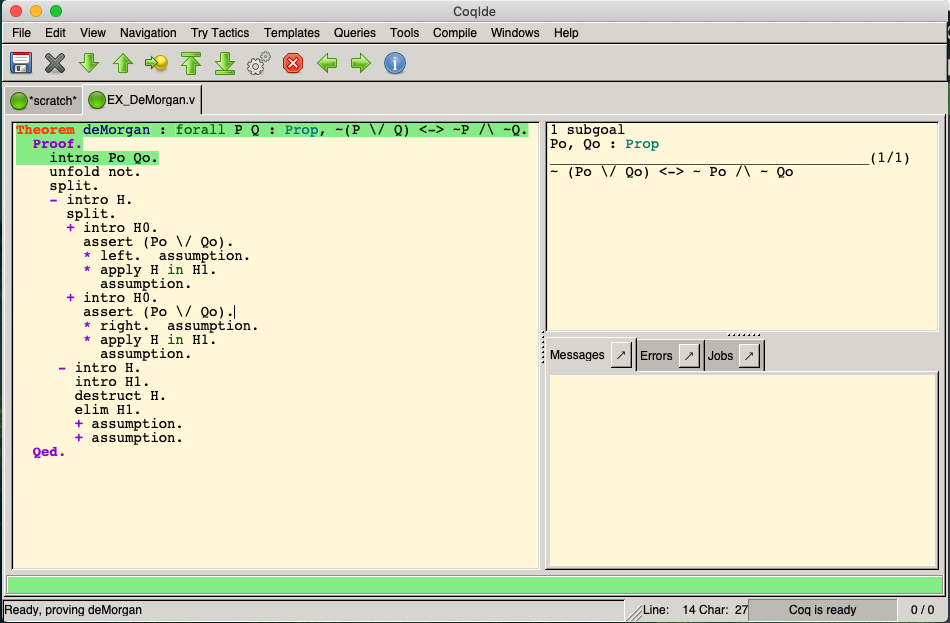
\includegraphics[scale=0.45]{DeMorgan}
              \caption{DeMorgan example, after \texttt{intros Po Qo}.}
    \label{fig:demorgan1st}
\end{figure}
        \par \medskip
        Next, we apply \texttt{unfold not}\footnote{Here, the tilde in Coq, equivalent to ``$\neg$" in our text, means ``not".  This step is not ``automatic"; the user has to realize that this is an appropriate next step in the proof.}  Since this is constructive logic, $\neg A$ is really just syntax sugar for $A \implies \bot$\footnote{The symbol $\bot$ is logical notation \cite{vanDalen} for ``False".  In constructive logic, negation is defined as such: ``not A" means ``A implies False".  For $\bot$ to be a proof goal means we are seeking a contradiction.  This means that to prove ``not A" can be reduced to proving that \emph{if} ``A" is assumed, then a contradiction can be derived, and so it cannot possibly be the case that ``A" is true.}.  This changes our singular goal to
        \[
        (P_0 \lor Q_0 \implies \bot) \Longleftrightarrow (P_0 \implies \bot) \land (Q_0 \implies \bot).
        \]
        We are now looking to prove a bi-implication, so we use \texttt{split}\footnote{Each command, as seen in the left window in the screen caps, was typed by the user.  We are executing them one line at a time.  The green highlighting shows which commands have already been executed, and the top-right window is the present proof state at that point.  The purpose of these screenshots is to show how the proof goal evolves with each step.} to split our one goal into two subgoals
        \begin{equation}\label{DMforward}
            (P_0 \lor Q_0 \implies \bot)\implies (P_0 \implies \bot) \land (Q_0 \implies \bot)
        \end{equation}
        and
        \begin{equation}\label{DMbackward}
            (P_0 \implies \bot) \land (Q_0 \implies \bot) \implies P_0 \land Q_0 \implies \bot.
        \end{equation}
        \par \medskip
        \noindent
\begin{figure}[H]
    \centering
          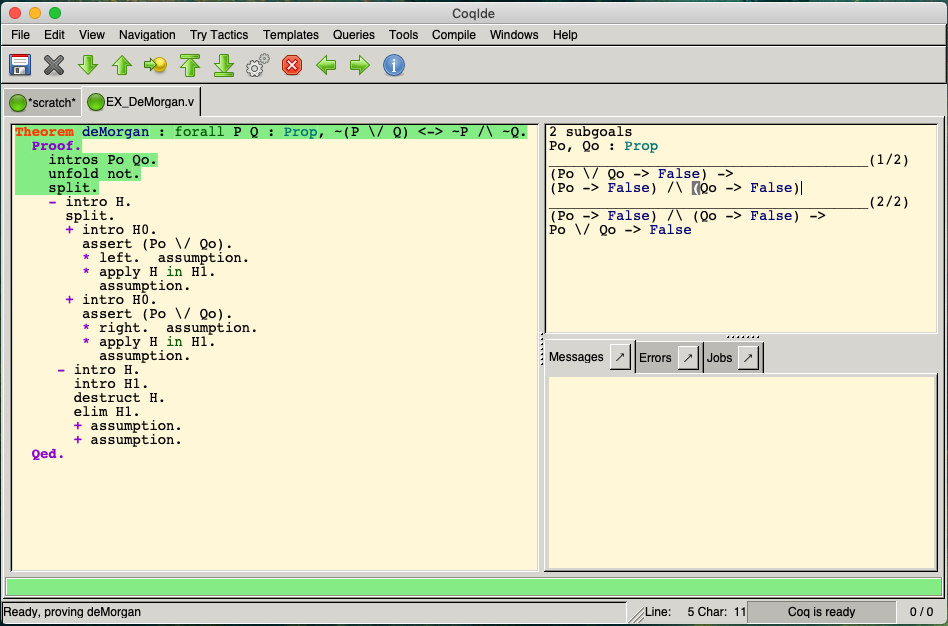
\includegraphics[scale=0.45]{DeMorgan2}
              \caption{DeMorgan example, after \texttt{split}.}
    \label{fig:demorgan1}
\end{figure}
        \par \medskip
        Since we have multiple subgoals now, we can use ``\texttt{-}" to \define{focus} the proof on only the first; so that we temporarily only worry about \eqref{DMforward}.  Focusing at deeper nested levels can be achieved by using ``\texttt{+}" and ``\texttt{*}"; if even more nesting is necessary (which is not the case in this proof), then one can start repeating the symbols, e.g. ``\texttt{-\,-}", ``\texttt{++}", and so on.
        \par After we focus, the primary goal is now \eqref{DMforward}, which is an implication; this requires us to assume the left-hand side in order to prove the right-hand side.  Using \texttt{intro H}, then, adds
        \[
            H : P_0 \lor Q_0 \implies \bot
        \]
        as a hypothesis, and changes the goal to 
        \[
            (P_0 \implies \bot) \land (Q_0 \implies \bot).
        \]
        Our goal is now a conjunction, so we use \texttt{split} to turn it into the two subgoals
        \begin{equation}\label{DMx1}
           P_0 \implies \bot
        \end{equation}
        and
        \begin{equation}\label{DMx2}
            Q_0 \implies \bot.
        \end{equation}
        \par \medskip
          \noindent
\begin{figure}[H]
    \centering
          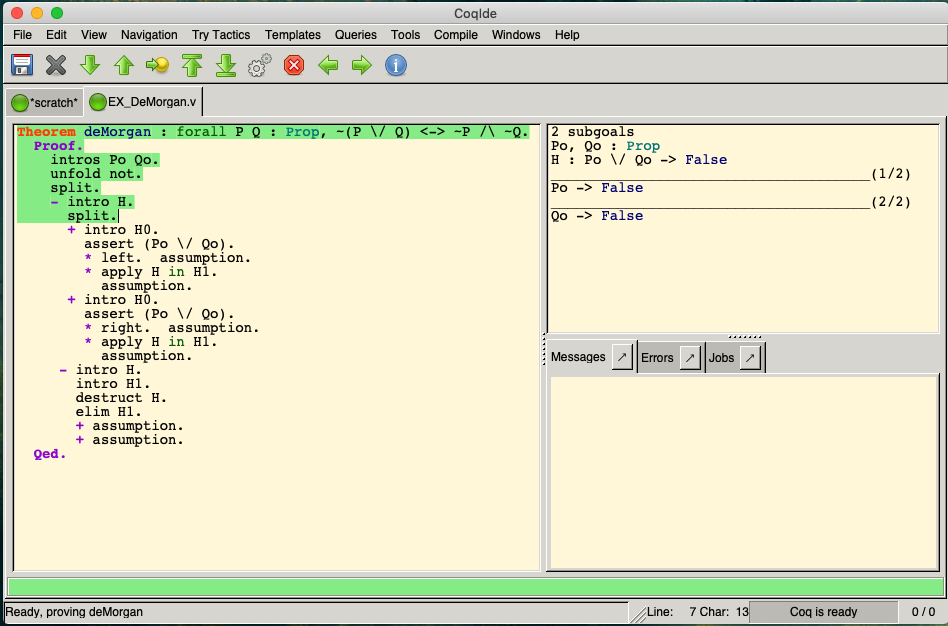
\includegraphics[scale=0.45]{DeMorgan3}
              \caption{DeMorgan example, after second \texttt{split}.}
    \label{fig:demorgan1}
\end{figure}
        \par \medskip
        We now use ``\texttt{+}" to focus on \eqref{DMx1}.  Again we have an implication, so \texttt{intro H0} adds the hypothesis 
        \[
            H_0 : P
        \]
        and gives us the remaining goal 
        \[
            \bot.
        \]
        We note that our existing hypothesis $H$ is an implication with $\bot$ as the conclusion, which can be invoked if we can prove the left-hand side $P_0 \lor Q_0$.  Thus, we use \texttt{assert (Po \textbackslash / Qo)}, which adds $P_0 \lor Q_0$ as a new goal.
        \par \medskip
          \noindent
\begin{figure}[H]
    \centering
          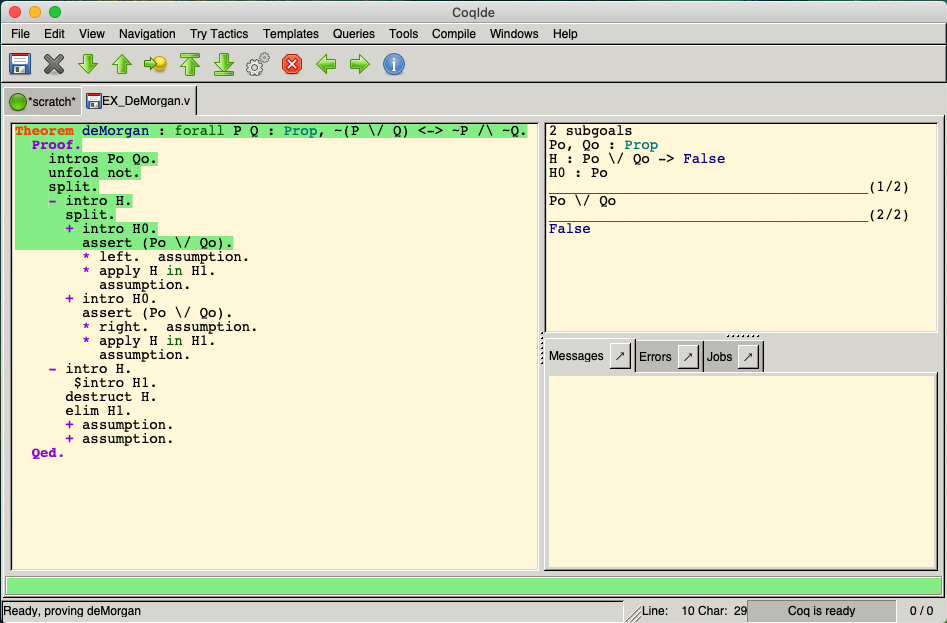
\includegraphics[scale=0.45]{DeMorgan4}
              \caption{DeMorgan example, after \texttt{assert}.}
    \label{fig:demorgan1}
\end{figure}
        \par \medskip
        We go another level deeper in focusing on the proof.  To prove a disjunction, it suffices to prove either the left or right hand side.  Since we already have $H_0 : P_0$ as a hypothesis, we apply the tactic \texttt{left}, which changes our goal to simply
        \[
         P_0.
        \]
        But now our goal is the same as something we already assumed, so \texttt{assumption}\index{assumption} dispatches it.
        \par We are now finished with this subgoal, and now are brought back one level up, to prove \eqref{DMx2}.
        \par \medskip
          \noindent
\begin{figure}[H]
    \centering
          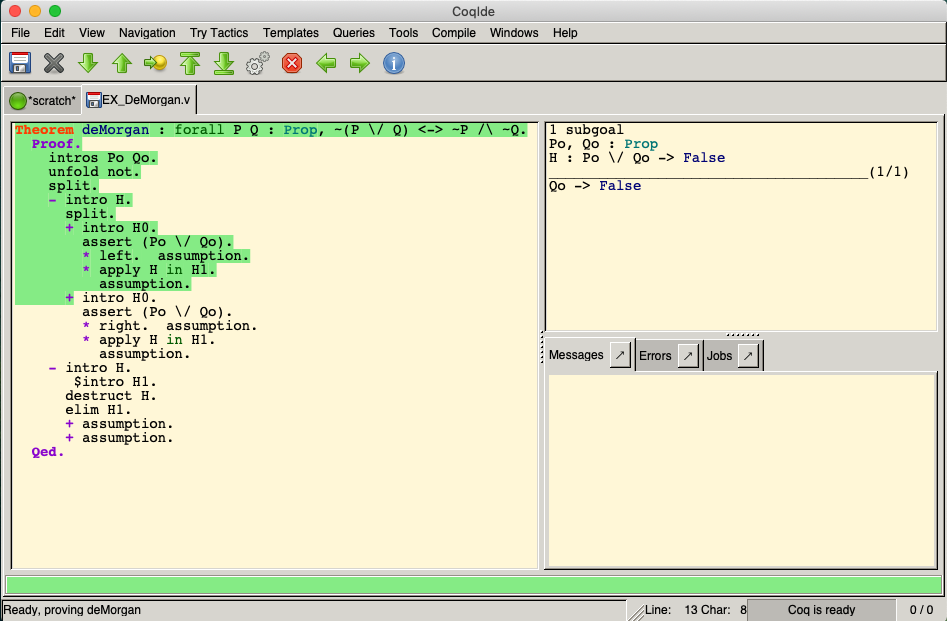
\includegraphics[scale=0.45]{DeMorgan5}
              \caption{DeMorgan example, after finishing proving \eqref{DMx1}.}
    \label{fig:demorgan1}
\end{figure}
        \par \medskip
        The proof of \eqref{DMx2} is analogous to \eqref{DMx1}, with the only difference being the use of \texttt{right} instead of \texttt{left}, to prove the other side of the disjunct $P_0 \lor Q_0$.  Thus, we omit the details and fast forward to returning to the original second subgoal \eqref{DMbackward}.
        \par \medskip
          \noindent
\begin{figure}[H]
    \centering
          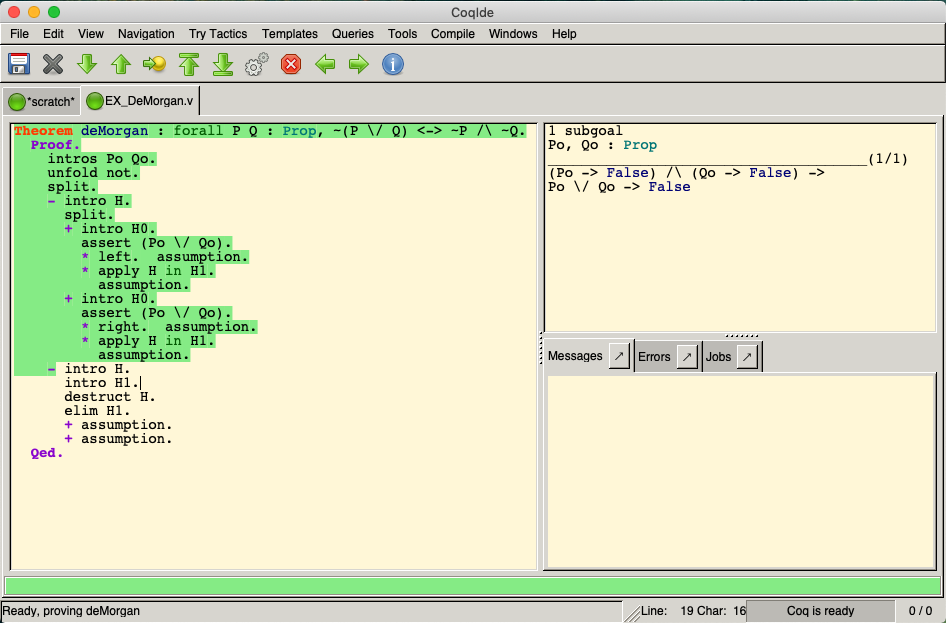
\includegraphics[scale=0.45]{DeMorgan6}
              \caption{DeMorgan example, after proving \eqref{DMx2}.}
    \label{fig:demorgan1}
\end{figure}
        \par \medskip
        When not explicitly bracketed, implication is right-associative, so what \eqref{DMbackward} really says is
        \[
            (P_0 \implies \bot) \land (Q_0 \implies \bot) \implies (P_0 \land Q_0 \implies \bot).
        \]
        We apply \texttt{intro} twice, adding
        \[
            H : (P_0 \implies \bot) \land (Q_0 \implies \bot)
        \]
        and
        \[
            H_1 : P_0 \land Q_0
        \]
        as hypotheses, and the goal becomes
        \[
            \bot.
        \]
        Next, as $H$ is a conjunction, it would be much more useful as a hypothesis if we break it down into its parts.  This is exactly what \texttt{destruct H} does, replacing $H$ with
        \[
            H : P_0 \implies \bot
        \]
        and
        \[
            H_0 : Q_0 \implies \bot.
        \]
        \par \medskip
          \noindent
\begin{figure}[H]
    \centering
          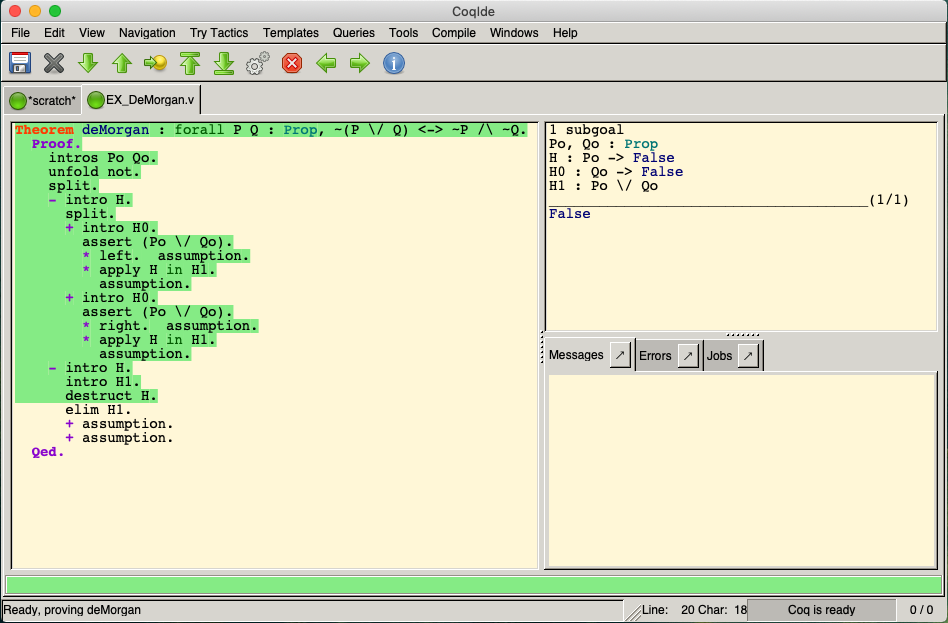
\includegraphics[scale=0.45]{DeMorgan7}
              \caption{DeMorgan example, after \texttt{destruct H}.}
    \label{fig:demorgan1}
\end{figure}
        \par \medskip
        We now turn to using our hypothesis $H_1 : P_0 \lor Q_0$.  This says that either the left or the right holds, we can reduce the goal to showing that either side implies it.  Using \texttt{elim H1} then changes the goals to
        \[
            P_0 \implies \bot
        \]
        and
        \[ 
            Q_0 \implies \bot.
        \]
        Both of these are already hypotheses, so are dispatched with \texttt{assumption}.
        \par This completes the proof, and by going past the line \texttt{Qed} in the proof window, we see in the output window
\begin{verbatim}
    deMorgan is defined
\end{verbatim}
        which tells us, in particular, that this theorem is now proven and \emph{saved} --- that is, it can be \define{applied} to future goals in this file (or another file by importing this one), where we can use it to  interchange $\neg(P\lor Q)$ with $\neg P \land \neg Q$ for any statements $P$ and $Q$ in any future proofs.
        \par \noindent
\begin{figure}[H]
    \centering
          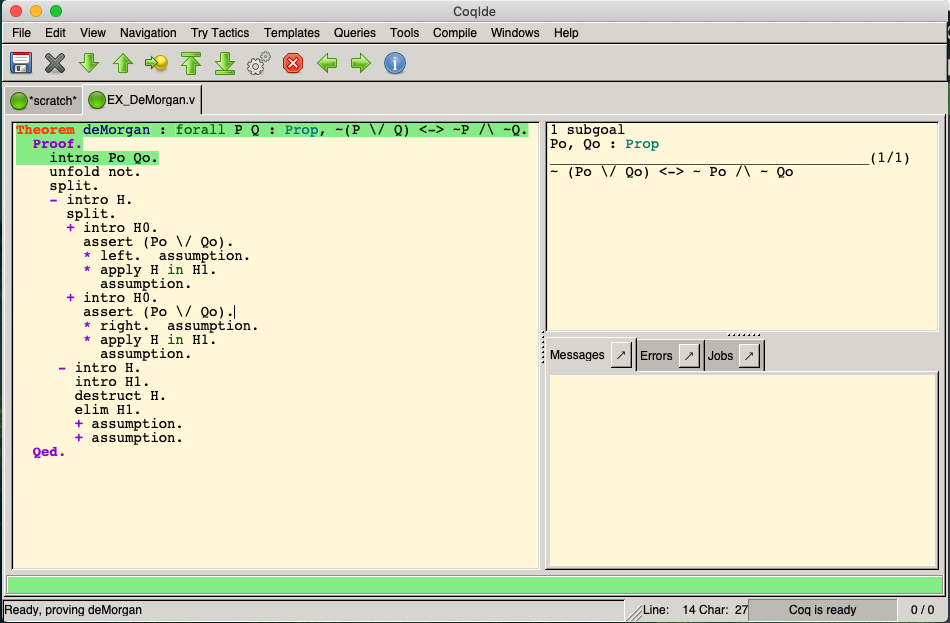
\includegraphics[scale=0.45]{DeMorgan}
              \caption{DeMorgan example, after completing the entire proof.}
    \label{fig:demorgan1}
\end{figure}
    \end{proof}
\end{theo}
It is worth repeating that the point of a proof is to compel belief (of the reader or user, in the validity of some particular statement) --- and with a formal proof in Coq the upshot is that, as they get longer and the details messier, it is not necessary for a reader to go through or understand every line to convince himself or herself that it is correct.  As long as the reader is convinced the statement of the theorem is correctly specified, is convinced of the validity of any added axioms or \define{admitted} proofs (this is when one does not finish the proof but simply tells Coq ``leave this and just trust that it's true") invoked, and believes that Coq itself is correct\footnote{All logical systems must start with some base of axioms accepted to be immutable truths, in order for anything to be derived.  We are still modelling with Coq based on some assumptions, and our proofs are not infallible --- but they add an additional layer of confidence and assurance.}, then they can be convinced that the proof is correct by executing past the \texttt{Qed} line.

\par As a remark, note that DeMorgan's \emph{other} theorem, namely that 
\[
    \neg (P \land Q) \Longleftrightarrow \neg P \lor \neg Q
\]
cannot be proven in the default logic of Coq, which is constructive.  That is, this proof relies on double negation
\[
    \neg\neg A \implies A,
\]
which is not a part of constructive logic.  However, one can, if one wishes, add this as an axiom\footnote{One must, of course, take care to not introduce inconsistent axioms if one's proofs are to have any meaning.  But in any event, it is always possible to trace back the use of any added axioms invoked in a proof.} in Coq and then proceed with the proof.

\section{Software Foundations --- the IMP language}
We now give the necessary definitions and theorems from Software Foundations \cite{Pier}, an interactive textbook on the mathematical foundations of reliable software, which is actually entirely a Coq script.

\par We use the \define{IMP} language defined within the Software Foundations Coq files for our code obfuscation formalisms.  IMP, which simply stands for imperative, is a bare-bones simple imperative language, like C stripped of all nonessential features.  This simplicity allows us to focus on the nuts and bolts of formally specifying and proving correct individual obfuscating transformations, emphasizing modularity.

\par Since IMP is written inside Coq, we can formally reason about not just individual programs, but entire classes of programs, and even the language itself.  We give the definitions, lemmas, and theorems necessary for our work, but will omit many details and proofs.  These can be found in full, either in the original text \cite{Pier}, or for convenience can also be found in the files prepended by ``SF" in the GitHub repository accompanying this thesis \cite{repo}.

\par IMP is built up piece by piece in \cite{Pier} with multiple iterations (some failed, some tangential) for pedagogical purposes, but we will only present the final form that we end up using.  IMP has the basics of natural number arithmetic, booleans, and commands consisting of assignment, skip, if-then-else, and while-do-end.

\subsection{Maps}\label{Maps}
The first library we use is \define{Maps}, the goal of which is to define a type of \define{total maps} with a default value for keys not present in the map.  These will be used to define program states later.

\begin{defin}[Total map]
    A \define{total map} over some type $A$ is a function from the type $string$ to $A$.  In Coq notation,
\begin{verbatim}
Definition total_map (A : Type) := string -> A.
\end{verbatim}
\end{defin}

\begin{defin}[Empty map]
    An \define{empty map}, given some default element $v$ of a type $A$, is a constant function that yields a map that returns $v$ when applied to any element of $A$.  In Coq notation,
\begin{verbatim}
Definition t_empty {A : Type} (v : A) : total_map A := (fun _ => v).
\end{verbatim}
\end{defin}

\begin{defin}[Update function]
    The \define{update function} takes a map $m$, a key (string) $x$, and value $v$, and returns a new map that sends $x$ to $v$ and all other keys to whatever $m$ originally did.  Intuitively, this is really just ``updating" a map at one key by a new value, but expressed in terms of higher-order programming.  The input to the update function is a map (itself a function), and outputs a new function.  In Coq notation,
\begin{verbatim}
Definition t_update {A : Type} (m : total_map A) (x : string) (v : A) :=
  fun x' => if eqb_string x x' then v else m x'.
\end{verbatim}
\end{defin}




\subsection{States}

\begin{defin}[State]
A \define{state}, for us, is simply a representation of \emph{all} variables at a point in time during the execution of an IMP program.  The variables' names are strings, and the values are natural numbers.  In practice, any particular program will only use finitely many variables, but to simplify the formalism we will simply let a state be a total map, with 0 as the default value for all variables.
\begin{verbatim}
Definition state := total_map nat.
\end{verbatim}
\end{defin}

Thus for us the ``default state" is the map \texttt{t\_empty 0} which sends every string to 0.  We then define some notation to make this easier to work with.

\begin{verbatim}
Notation "{ --> d }" := (t_empty d) (at level 0).
\end{verbatim}

With this, \texttt{"\{ --> 0\}"} becomes shorthand for the empty map.  The \texttt{level 0} declares the associativity precedence of the notation (e.g. multiplication is evaluated before addition in the absence of brackets), with lower number meaning higher precedence.  We can now create readable short hand for arbitrary states as follows.

\begin{verbatim}
Notation "{ a --> x }" := (t_update { --> 0 } a x) (at level 0).
Notation "{ a --> x ; b --> y }" := (t_update ({ a --> x }) b y) (at level 0).
Notation "{ a --> x ; b --> y ; c --> z }" := 
    (t_update ({ a --> x ; b --> y }) c z) (at level 0). 
etc...
\end{verbatim}

For instance, the state denoted by \texttt{\{ X --> 1 ; Y --> 2 ; Z --> 0 \}} is the function that maps $X$ to 1, $Y$ to 2, $Z$ to 0, and all other strings to 0.

\par Additionally, notation is defined such that we can write \texttt{m \& \{ X --> 1 ; Y --> 2 ; Z --> 0 \}} to mean some state $m$ updated with the mappings $X$ to 1, $Y$ to 2, $Z$ to 0.

\subsection{Arithmetic and boolean expressions}
We first give a brief explanation of \define{currying} to explain the preferred syntax in Coq for denoting functions with multiple arguments.  Coq is, first of all, right-associative by default, so that
\[
    A \to B \to C
\]
without brackets implicitly means
\[
    A \to (B \to C).
\]
Moreover, there is a natural isomorphism as sets of functions\footnote{Here, $\times$ is the cartesian product of sets.  An arrow indicates the set of functions between sets; i.e.\ $A\to B$ is the set of all functions from $A \to B$. \par The symbol $\cong$ indicates there is an \emph{isomorphism} between the set on the left and the set on the right.  They are not \emph{literally} the same sets, but there is a bijective (one-to-one and onto) correspondance between their elements.}
\[
    (A \times B) \to C \cong A \to (B \to C).
\]
Given a function $f \in (A \times B) \to C$, we can define\footnote{An element of the set $A\to (B \to C)$ is a function which takes an element of $A$ and outputs a function from $B$ to $C$.  The symbol $\mapsto$ means ``maps to" or and indicates the action of a function on an element. \par Unpacking this definition entirely into plain English would say, ``Given a function from $f$ from $(A\times B)$ to $C$, we define a function $h$ from $A$ to $(B\to C)$ defined as follows.  For any $a \in A$, $h(a)$ is the function from $B$ to $C$ which sends any $b\in B$ to $f(a,b)$.  So, $h(a)(b)=f(a,b)$."}
\begin{align*}
    h: A &\to (B \to C), \\
        a &\mapsto (b \mapsto f(a,b)).
\end{align*}
This extends to any number of types, so that function of a type
\[
    A_1 \to A_2 \to A_3 \to \ldots \to A_n
\]
should intuitively be thought of as a function
\[
    (A_1 \times A_2 \times \ldots \times A_{n-1}) \to A_n,
\]
with the additional expressive power that one need not necessarily go ``all the way".  For example, a function of type
\[
    A \to B \to C \to D
\]
would output an element of type $D$ if fed inputs of types $A$, $B$, and $C$.  However, feeding it only inputs of type $A$ and $B$ would then output a function of type $C \to D$.

\begin{defin}[Arithmetic expression]
    \define{Arithmetic expressions} are defined as an \define{inductive type} as follows.
\begin{verbatim}
Inductive aexp : Type :=
  | ANum : nat -> aexp
  | AId : string -> aexp
  | APlus : aexp -> aexp -> aexp
  | AMinus : aexp -> aexp -> aexp
  | AMult : aexp -> aexp -> aexp.
\end{verbatim}
What this says is that for any natural number $n$, \texttt{ANum n} is an \texttt{aexp} which represents that number.  For any string $x$, \texttt{AId x} is an \texttt{aexp} which represents the variable $x$.  Then, for any existing arithmetic expressions $a1$ and $a2$, we can build new arithmetic expressions representing their addition (\texttt{APlus a1 a2}), subtraction (\texttt{AMinus a1 a2}), or multiplication (\texttt{AMult a1 a2}).
\par For example, the arithmetic expression $(x + 5) * (3 - 2)$ would formally thus be
\begin{verbatim}
AMult (APlus (AId x) (ANum 5)) (AMinus (ANum 3) (ANum 2)).
\end{verbatim}
Of course, in practice this would quickly get very annoying and very unreadable, so some notational tricks allow us to henceforth use the human notation familiar from kindergarten.
\begin{verbatim}
Coercion AId : string >-> aexp.
Coercion ANum : nat >-> aexp.
Bind Scope aexp_scope with aexp.
Infix "+" := APlus : aexp_scope.
Infix "-" := AMinus : aexp_scope.
Infix "*" := AMult : aexp_scope.
\end{verbatim}
\end{defin}

\begin{defin}[Boolean expression]
    \define{Boolean expressions} are also an inductive type, as follows.
\begin{verbatim}
Inductive bexp : Type :=
  | BTrue : bexp
  | BFalse : bexp
  | BEq : aexp -> aexp -> bexp
  | BLe : aexp -> aexp -> bexp
  | BNot : bexp -> bexp
  | BAnd : bexp -> bexp -> bexp.
\end{verbatim}
Here, \texttt{BTrue} and \texttt{BFalse} represent the constants for true and false, respectively.  Given two arithmetic expressions $a1$ and $a2$, new boolean expressions can be formed, \texttt{BEq a1 a2} (equality) and \texttt{BLe a1 a2} (less than or equals to).  Finally, \texttt{BNot} and \texttt{BAnd} form new boolean expressions corresponding to negation and conjunction, respectively.  Thanks to DeMorgan's Theorem, disjunction can be defined in terms of negation and conjunction, thus need not be part of the formal inductive definition.
\par Once again, some notational declarations allow us to henceforth use familiar infix notation for boolean expressions as well.
\begin{verbatim}
Definition bool_to_bexp (b: bool) : bexp := if b then BTrue else BFalse.
Coercion bool_to_bexp : bool >-> bexp.
Bind Scope bexp_scope with bexp.
Infix "<=" := BLe : bexp_scope.
Infix "=" := BEq : bexp_scope.
Infix "&&" := BAnd : bexp_scope.
Notation "'!' b" := (BNot b) (at level 60) : bexp_scope.
\end{verbatim}
\end{defin}

Note that all we have done so far is define the \define{abstract syntax} of arithmetic and boolean expressions.  That is, we have defined two types \texttt{aexp} and \texttt{bexp} and the rules for inductively generating all the elements of those types that we will need for the IMP language, but at this point they do not yet have any meaning.

\par Given a particular state and a particular arithmetic expression or a particular boolean expression, the following yield a natural (\texttt{nat}) or boolean (\texttt{bool}) value, respectively, which that abstract expression evaluates to in the given program state.

\begin{defin}[Arithmetic evaluation function]\label{aritheval}
The \define{arithmetic evaluation function} is
\begin{verbatim}
Fixpoint aeval (st : state) (a : aexp) : nat :=
  match a with
  | ANum n => n
  | AId x => st x                               
  | APlus a1 a2 => (aeval st a1) + (aeval st a2)
  | AMinus a1 a2  => (aeval st a1) - (aeval st a2)
  | AMult a1 a2 => (aeval st a1) * (aeval st a2)
  end.\end{verbatim}
\end{defin}

\begin{example}
As a concrete example, suppose we have a state \texttt{st} where the value of $x$ is 1 and the value of $y$ is 2.  Suppose we have an arithmethic expression 
\begin{verbatim}
AMult (ANum 3) (APlus (AId x) (AId y)
\end{verbatim}
which represents $3 * (x + y)$ in ordinary math notation.  We want to evaluate this expression in the state \texttt{st}.  \par We compute 
\begin{verbatim}
aeval st (AMult (ANum 3) (APlus (AId x) (AId y))).
\end{verbatim}
At the top level there is a multiplication.  This is matched to the \texttt{AMult} case and resolves to 
\begin{verbatim}
(aeval st (ANum 3) * (aeval st (APlus (AId x) (AId y))).  
\end{verbatim}
\par Next, the left-hand side is a constant (\texttt{ANum 3}) which is just mapped to the number 3, so now are at 
\begin{verbatim}
3 * (aeval st (APlus (AId x) (AId y))).
\end{verbatim}
\par Next, we have an addition, \texttt{APlus}, so we now are at 
\begin{verbatim}
3 * ((aeval st (AId x)) + aeval (st (AId y)).
\end{verbatim}
The two remaining evaluations are looking up the values of the variables $x$ and $y$ in our given state, so we finally arrive at 
\begin{verbatim}
3 * (1 + 2). 
\end{verbatim}
This is now an expression purely in the natural numbers, and simplifies to $9$.
\end{example}

\begin{defin}[Boolean evaluation function]
The \define{boolean evaluation function} is
\begin{verbatim}
Fixpoint beval (st : state) (b : bexp) : bool :=
  match b with
  | BTrue => true
  | BFalse => false
  | BEq a1 a2 => (aeval st a1) =? (aeval st a2)
  | BLe a1 a2 => (aeval st a1) <=? (aeval st a2)
  | BNot b1 => negb (beval st b1)
  | BAnd b1 b2 => andb (beval st b1) (beval st b2)
  end.
\end{verbatim}
The infix notation \texttt{=?} is for the function of type \texttt{nat -> nat -> bool} that returns true if and only if the two natural numbers given as arguments are equal.  Similarly, \texttt{<=?} is the same for less than or equals.
\par The \texttt{negb} and \texttt{andb} functions are the negation and conjunction on booleans, respectively, of type \texttt{bool -> bool} and \texttt{bool -> bool -> bool}.  These boolean values are analogous to those found in more familiar programming languages and meant to represent actual truth values, whereas the syntax \verb$/\$ and \texttt{not} introduced in Theorem \ref{DeMorgan} were for \emph{propositions} (of type \texttt{Prop}) to be reasoned about.
\end{defin}

Otherwise, these evaluation functions should be fairly self-explanatory; the \define{fixpoint} declaration denotes a recursive (but terminating) function.  Coq has a built-in termination checker that will complain if it cannot detect a strictly decreasing argument in the parameters.  In this case, it can tell that \texttt{aexp} or \texttt{bexp} shrinks in complexity on each recursively invoked iteration.

\subsection{Commands}
We can now define the abstract syntax of \define{commands}, or IMP programs proper.

\begin{defin}[(IMP) command]\label{impcommand}
    The following is an inductive definition of a \emph{command}.
    \begin{verbatim}
Inductive com : Type :=
  | CSkip : com
  | CAss : string -> aexp -> com
  | CSeq : com -> com -> com
  | CIf : bexp -> com -> com -> com
  | CWhile : bexp -> com -> com.
    \end{verbatim}
    The notation declarations to make this easier to work with are as follows.
\begin{verbatim}
Bind Scope com_scope with com.
Notation "'SKIP'" := CSkip : com_scope.
Notation "x '::=' a" := (CAss x a) (at level 60) : com_scope.
Notation "c1 ;; c2" :=
  (CSeq c1 c2) (at level 80, right associativity) : com_scope.
Notation "'WHILE' b 'DO' c 'END'" :=
  (CWhile b c) (at level 80, right associativity) : com_scope.
Notation "'IFB' c1 'THEN' c2 'ELSE' c3 'FI'" :=
  (CIf c1 c2 c3) (at level 80, right associativity) : com_scope.
\end{verbatim}
\end{defin}

\begin{comment}
\begin{example}[Factorial program in Coq]
    With the defined notation, we can write IMP programs in a relatively human-readable way.  The following is a program that considers $X$ as an input, uses $Z$ as a temporary variable, and outputs the factorial of $X$ as $Y$.
    \begin{verbatim}
Definition fact_in_coq : com :=
  Z ::= X;;
  Y ::= 1;;
  WHILE ! (Z = 0) DO
    Y ::= Y * Z;;
    Z ::= Z - 1 
  END.
    \end{verbatim}
\end{example}
\end{comment}

We now define evaluation of a command.  While arithmetic and boolean evaluation could be defined as functions, we cannot do the same for commands.  Due to the existence of While loops, they may not terminate, and thus we cannot write a recursive \texttt{Fixpoint} function in Coq.  Instead, we must define the evaluation of commands as \emph{relations}.  The disadvantage of this, however, is that Coq can no longer just take an abstract expression and compute its output - we must construct proofs ourselves that a particular relation holds --- that is, that a program will evaluate from a particular start state to a particular final state.
\par In the following definition, \texttt{Reserved Notation}\index{reserved notation} allows us to pre-define the notation for command evaluation, so that it can be used in the writing of the definition itself.\footnote{That is, this allows us to use shorthand notation for \texttt{ceval} while we are still defining \texttt{ceval}.  If we didn't have this line, we would have to write things like \texttt{(ceval c1 st st')} throughout the definition instead of \texttt{c1 / st  \textbackslash\textbackslash\ st'}.}

\begin{defin}[Command evaluation]\label{commeval}
The \define{command evaluation} relation is inductively defined as follows.
\begin{verbatim}
Reserved Notation "c1 '/' st '\\' st'" (at level 40, st at level 39).

Inductive ceval : com -> state -> state -> Prop :=
  | E_Skip : forall st,
      SKIP / st \\ st
  | E_Ass  : forall st a1 n x,
      aeval st a1 = n ->
      (x ::= a1) / st \\ st & { x --> n }
  | E_Seq : forall c1 c2 st st' st'',
      c1 / st  \\ st' ->
      c2 / st' \\ st'' ->
      (c1 ;; c2) / st \\ st''
  | E_IfTrue : forall st st' b c1 c2,
      beval st b = true ->
      c1 / st \\ st' ->
      (IFB b THEN c1 ELSE c2 FI) / st \\ st'
  | E_IfFalse : forall st st' b c1 c2,
      beval st b = false ->
      c2 / st \\ st' ->
      (IFB b THEN c1 ELSE c2 FI) / st \\ st'
  | E_WhileFalse : forall b st c,
      beval st b = false ->
      (WHILE b DO c END) / st \\ st
  | E_WhileTrue : forall st st' st'' b c,
      beval st b = true ->
      c / st \\ st' ->
      (WHILE b DO c END) / st' \\ st'' ->
      (WHILE b DO c END) / st \\ st''

  where "c1 '/' st '\\' st'" := (ceval c1 st st').
\end{verbatim}
Intuitively, \verb$c1 / st \\ st'$ means ``the program $c1$ takes the initial state $st$ to the final state $st'$".  
\par We also give the rules of evaluation informally as logical inference rules for readability.  Most are immediately obvious, but the While rules are worth explaining.
\par The E\_WhileTrue rule describes what happens when the guard condition $b$ is true, and we go through one iteration of a loop.  If, when $b$ evaluates to true, it is the case that $c$ takes $st$ to $st'$ (the current iteration), and the main While statement takes $st'$ to $st''$ (the remaining iterations after the current one), then it can be concluded that the main While statement takes $st$ to $st''$ (putting together the current iteration with the remaining iterations).  On the other hand, to prove that the loop terminates, we'll have to have applied E\_WhileTrue until the condition $b$ is now false, whence the E\_WhileFalse rule says to not enter the loop again (it takes a state $st$ to itself, reflecting that nothing has happened).
\end{defin}

\[
  \begin{prooftree}
    \Infer1[E\_Skip]{SKIP\ /\ st\ \backslash\backslash\ st}
  \end{prooftree}
\]

\[
  \begin{prooftree}
    \Hypo{aeval\ st\ a1=n}
    \Infer1[E\_Ass]{x := a1\ /\ st\ \backslash\backslash\ st\ \&\ \{ x \to n \}}
  \end{prooftree}
\]

\[
  \begin{prooftree}
    \Hypo{c1\ /\ st\ \backslash\backslash\ st'}\Hypo{c2\ /\ st'\ \backslash\backslash\ st''}
    \Infer2[E\_Seq]{c1;;c2\ /\ st\ \backslash\backslash\ st''}
  \end{prooftree}
\]

\[
  \begin{prooftree}
    \Hypo{beval\ st\ b1=true}\Hypo{c1\ /\ st\ \backslash\backslash\ st'}
    \Infer2[E\_IfTrue]{IF\ b1\ THEN\ c1\ ELSE\ c2\ FI\ /\ st\ \backslash\backslash\ st'}
  \end{prooftree}
\]

\[
  \begin{prooftree}
    \Hypo{beval\ st\ b1=false}\Hypo{c2\ /\ st\ \backslash\backslash\ st'}
    \Infer2[E\_IfFalse]{IF\ b1\ THEN\ c1\ ELSE\ c2\ FI\ /\ st\ \backslash\backslash\ st'}
  \end{prooftree}
\]

\[
  \begin{prooftree}
    \Hypo{beval\ st\ b=false}
    \Infer2[E\_WhileFalse]{WHILE\ b\ DO\ c\ END\ /\ st\ \backslash\backslash\ st}
  \end{prooftree}
\]

\[
  \begin{prooftree}
    \Hypo{beval\ st\ b=true}\Hypo{c\ /\ st\ \backslash\backslash\ st'}
    \Infer[rule style=no rule]2{WHILE\ b\ DO\ c\ END\ /\ st'\ \backslash\backslash\ st''}
    \Infer2[E\_WhileTrue]{WHILE\ b\ DO\ c\ END\ /\ st\ \backslash\backslash\ st''}
  \end{prooftree}
\]

\subsection{Equivalence}

\begin{defin}[Arithmetic/boolean expression equivalence]\index{arithmetic equivalence}\index{boolean equivalence}
    For two arithmetic, respectively boolean, expressions to be equivalent means that in all states, they evaluate to the same natural number, respectively boolean value.  In Coq,
\begin{verbatim}
Definition aequiv (a1 a2 : aexp) : Prop := 
  forall (st:state), aeval st a1 = aeval st a2.

Definition bequiv (b1 b2 : bexp) : Prop := 
  forall (st:state), beval st b1 = beval st b2.
\end{verbatim}
\end{defin}

\begin{defin}[Command equivalence]\label{commequiv} \index{command equivalence}
    For two commands (IMP programs) $c_1$ and $c_2$ to be equivalent means that for any pair of states $st$ and $st'$, $c_1$ takes $st$ to $st'$ if and only if $c_2$ takes $st$ to $st'$.  In Coq,
\begin{verbatim}
Definition cequiv (c1 c2 : com) : Prop :=
  forall (st st' : state), (c1 / st \\ st') <-> (c2 / st \\ st').
\end{verbatim}
\end{defin}

\subsection{Hoare logic}
\define{Hoare logic} is a way for us to prove that executing a program will result in satisfying certain post-conditions, (possibly) conditional on certain pre-conditions being met.  This involves defining a natural way of writing program specifications, along with a compositional proof technique to prove correctness with respect to them.
\begin{defin}[Hoare triple]
	A \define{Hoare triple}, which we sometimes refer to simply as a triple, consists of a pre-condition $P$, a program $c$, and a post-condition $Q$, written
    \[
    	(| P |)\ c\ (| Q |),
    \]
    which specifies that whenever $P$ is true before execution, running the program $c$ is guaranteed to make $Q$ true after execution.  This informal definition leaves states implicit, but for the formulation in Coq we will need to take states into account.
\end{defin}

\begin{defin}[Assertion]
An \define{assertion} about a program's state, formally, is a function from states to propositions.
\begin{verbatim}Definition Assertion := state -> Prop.\end{verbatim}
Informally, for some assertion $P$ and some state $st$, the proposition $P(st)$ represents the statement that $P$ holds in state $st$.  
\par As an example, let $st$ be the state where the value of every variable is 0.  Let $P$ be the assertion that $x=0$.  Then $P(st)$ is the proposition ``$x = 0$ in the state $st$".
\end{defin}

\begin{defin}[Assertion implication]\label{assertimplies}\index{assertion implication}
Given assertions $P$ and $Q$, to say that $P$ implies $Q$ means that whenever $P$ holds in some given state, so does $Q$.  The definition and shorthand notation in Coq is given below.
\begin{verbatim}
Definition assert_implies (P Q : Assertion) : Prop :=
  forall st, P st -> Q st.

Notation "P ->> Q" := (assert_implies P Q)
  (at level 80) : hoare_spec_scope.
\end{verbatim}
  
 There is also notation defined for bidirectional assertion implication, wherein one can write ``\texttt{P <<->> Q}" to mean ``both \texttt{P ->> Q} and \texttt{Q ->> P}."
\begin{verbatim}
Notation "P <<->> Q" :=
  (P ->> Q /\ Q ->> P) (at level 80) : hoare_spec_scope.
\end{verbatim}
\end{defin}

\begin{defin}[Hoare triple (in Coq)]
A Hoare triple is defined in Coq as follows, taking states into account.
\begin{verbatim}
Definition hoare_triple (P:Assertion) (c:com) (Q:Assertion) : Prop :=
  forall st st', c / st \\ st'  -> P st -> Q st'.
  
Notation "{{ P }}  c  {{ Q }}" :=
  (hoare_triple P c Q) (at level 90, c at next level) : hoare_spec_scope.
\end{verbatim}
\end{defin}

Proving that a Hoare triple holds is a line-by-line affair, starting from the bottom of a program and working upwards.  There is one rule for each kind of IMP command, and the application is mostly mechanical.  We give the definitions of the rules as presented in \cite{Pier} below, both as informal logical inference rules and the definition (informally we refer to the rules as definitions, but in Coq they are stated as theorems that the rule is correct and can be applied --- for brevity we won't repeat the proofs here) in Coq.

\begin{defin}[Hoare logic assignment rule]\label{hoareassign}\index{Hoare logic!assignment rule}
\[
  \begin{prooftree}
    \Infer1[hoare\_asgn]{(| Q [X\mapsto a] |)\ X::=a \ (|Q|)}
  \end{prooftree}
\]
\begin{verbatim}
Definition assn_sub X a P : Assertion :=
  fun (st : state) => P (st & { X  --> aeval st a }).

Notation "P [ X |-> a ]" := (assn_sub X a P) (at level 10).

Theorem hoare_asgn : forall Q X a, {{Q [X |-> a]}} (X ::= a) {{Q}}.
\end{verbatim}
Intuitively, \verb$assn_sub X a P$ is the assertion whose action on states is given by taking the existing assertion \verb$P $and first updating the state with the assignment \verb${X --> aeval st a}$.
\end{defin}

\begin{defin}[Hoare logic consequence rule]\label{hoareconsequence}\index{Hoare logic!consequence rule}
\[
  \begin{prooftree}
    \Hypo{(|P'|)\ c\ (|Q'|)}\Hypo{P \twoheadrightarrow P'}\Hypo{Q' \twoheadrightarrow Q}
    \Infer3[hoare\_consequence]{[(|P|)\ c\ (|Q|)}
  \end{prooftree}
\]

The consequence rule allows us to strengthen pre-conditions and/or weaken post-conditions.  In Coq, there are separate rules for the two.

\begin{verbatim}
Theorem hoare_consequence_pre : forall (P P' Q : Assertion) c,
  {{P'}} c {{Q}} -> P ->> P' -> {{P}} c {{Q}}.
  
Theorem hoare_consequence_post : forall (P Q Q' : Assertion) c,
  {{P}} c {{Q'}} -> Q' ->> Q -> {{P}} c {{Q}}.
\end{verbatim}
\end{defin}

\begin{defin}[Hoare logic skip rule]\label{hoareskip}\index{Hoare logic!skip rule}
\[
  \begin{prooftree}
    \Infer1[hoare\_skip]{(| P |)\ SKIP \ (|P|)}
  \end{prooftree}
\]
\begin{verbatim}Theorem hoare_skip : forall P, {{P}} SKIP {{P}}.\end{verbatim}
\end{defin}

\begin{defin}[Hoare logic sequencing rule]\label{hoareseq}\index{Hoare logic!sequencing rule}
\[
  \begin{prooftree}
    \Hypo{(|P|)\ c_1\ (|Q|)}\Hypo{(|Q|)\ c_2\ (|R|)}
    \Infer2[hoare\_seq]{[(|P|)\ c_1;;c_2\ (|R|)}
  \end{prooftree}
\]
\begin{verbatim}
Theorem hoare_seq : forall P Q R c1 c2,
  {{Q}} c2 {{R}} -> {{P}} c1 {{Q}} -> {{P}} c1;;c2 {{R}}.
\end{verbatim}
\end{defin}

\begin{defin}[Hoare logic conditional rule]\label{hoareif}\index{Hoare logic!conditional rule}
\[
  \begin{prooftree}
    \Hypo{(|P \land b|)\ c_1\ (|Q|)}\Hypo{(|P \land \neg b|)\ c_2\ (|Q|)}
    \Infer2[hoare\_if]{[(|P|)\ IFB\ b\ THEN\ c_1\ ELSE\ c_2\ FI\ (|Q|)}
  \end{prooftree}
\]
\begin{verbatim}
Definition bassn b : Assertion := fun st => (beval st b = true).

Theorem hoare_if : forall P Q b c1 c2,
  {{fun st => P st /\ bassn b st}} c1 {{Q}} ->
  {{fun st => P st /\ ~(bassn b st)}} c2 {{Q}} ->
  {{P}} (IFB b THEN c1 ELSE c2 FI) {{Q}}.
\end{verbatim}
\end{defin}

\begin{defin}[Hoare logic while rule]\label{hoarewhile}\index{Hoare logic!while rule}
\[
  \begin{prooftree}
    \Hypo{(|P \land b|)\ c\ (|P|)}
    \Infer2[hoare\_while]{[(|P|)\ WHILE\ b\ DO\ c\ END\ (|P \land \neg b|)}
  \end{prooftree}
\]
\begin{verbatim}
Theorem hoare_while : forall P b c,
  {{fun st => P st /\ bassn b st}} c {{P}} ->
  {{P}} WHILE b DO c END {{fun st => P st /\ ~ (bassn b st)}}.
\end{verbatim}
\end{defin}
The two items that may not be immediately intuitive, and indeed the only ones that are not completely mechanical, are the \emph{while} rule and the \emph{consequence} rule.  The while rule requires a \define{loop invariant}, a boolean statement $b$ (wrapped up into an assertion that $b$ evaluates to true in a given state), that is true throughout each iteration of the loop and no longer true once the loop terminates.  \par The \emph{consequence} rule, on the other hand, is used to either strengthen the pre-condition or weaken the post-condition, which may a priori not be in the exact form required for the rest of the intermediary proof.

\par A detailed treatment of Hoare logic can be found in \cite{HuRy}.

\begin{comment}
\section{List of Coq Tactics}
In this section we provide a complete reference list of Coq tactics used throughout the remainder of this thesis.
\end{comment}



 \chapter{Opaque predicates in IMP/Coq}

We now enter the main topic of the thesis proper, formalizing and certifying the opaque predicate transformation introduced in Section \ref{motivating}.  Recall that this transformation takes as inputs a program to be obfuscated, $c_1$, an opaque predicate $P$, and a dummy program\footnote{It's not known to an attacker, a priori, that it's a dummy program.  In practice, $c_2$ should be constructed so that it is not obvious; e.g.\ $c_2$ should not be simply an empty program, but should be complicated enough that it looks like it could feasibly be intended to be executed.} $c_2$, and returns the program
\begin{verbatim}
    IFB (P x) THEN c1 ELSE c2 FI.
\end{verbatim}

\par In the Section \ref{naive}, we describe our initial (straightforward, naive) attempt, explicitly defining the transformation to introduce the lines of code that assign variables associated with the opaque predicate (as one may naturally expect to write code in a typical imperative language), and see that trying to state a general theorem about command equivalence ends up being problematic.  
\par However, we then discuss how this spawned two ideas in different directions that rectify the issue.  On the one hand, we use Hoare logic with this first formulation, in Section \ref{hoarequiv}, to prove weaker conditions of a transformation than total command equivalence.  On the other hand, in Section \ref{noass} we reformulate the transformation to rely on values already existing in the state of the program, with the view that one may be applying an opaque predicate transformation to a small piece of code somewhere within a much larger program that would have such values floating around in the state already.
\par Finally in Section \ref{weakened}, we again employ Hoare logic to give a formal example of how an attacker who does not know about the opaque predicate's constant truth valuation, but otherwise can analyze (using static analysis) the program, ends up gaining weaker knowledge because of it.
\par All code for this chapter is in the file \verb$OBFS_opaque_predicate.v$ \cite{repo}.

\section{Command equivalence}\label{naive}
\begin{defin}[Factorial program (countdown nonzero formulation)]\label{Fact}\index{factorial program!countdown nonzero formulation}
    The following IMP program computes the factorial of a nonzero natural number.  The input is read from $X$, temporary values are stored as $Z$, and the factorial of the input is stored in $Y$ as the output.
\begin{verbatim}
Definition fact_nonzero : com :=
  Z ::= X;;
  Y ::= 1;;
  WHILE ! (Z <= 1) DO
    Y ::= Y * Z;;
    Z ::= Z - 1
  END.
\end{verbatim}
\end{defin}

\begin{rem}
    The choice of factorial program as a candidate for examples of obfuscation is somewhat arbitrary.  It works well for illustrative purposes, however, as it is neither too complex nor completely trivial.
\end{rem}

\begin{example}\label{firstoff}
    The \verb$fact_nonzero$ program with input $X=3$ yields output $Y=6$.  However, the story is not quite so simple (it is true that input $X=3$ yields $Y=6$, but as one can see in the Coq example, the state keeps track of the value of every variable involved in the program.).  The specification of this statement in Coq is
\begin{verbatim}
Example factorial_3: fact_nonzero / { X --> 3 } \\
  { X --> 3; Z --> 3; Y --> 1; Y --> 3; Z --> 2; Y --> 6; Z --> 1 }.
\end{verbatim}
    Note that formally, the final state holds the information of every intermediate assignment made by the program.  We can discern the output $Y=6$ by the fact that this is the rightmost case of a value being assigned to $Y$.  But wait, there's more!  We said earlier that in Coq, an example is no different from a proposition or a theorem in anything but name, so we must actually give a proof\footnote{This really is an example, to us.  But just because one declares ``here is an example of $X$" does not mean that $X$ is necessarily true.  In Coq, a proof must still be constructed.\par For example, in natural language, one can say ``An example of a prime number is 20051".  But this isn't immediately obvious, and one still needs to prove that example, for instance, by writing a program that tries to divide it by every number up to its square root.}.  Moreover, since command evaluation is relational and not functional (recall the reason for this is the possibility of non-terminating While loops), we must build the proof out step by step.
    \begin{proof}
        We give a screenshot of the Coq code, and describe the main points of interest, in particular explaining any concepts and proof tactics not seen prior.  As we explained and gave the reasoning for in Section \ref{proofexplain}, there will be some steps in this and all future proofs that are not discussed in detail.
        
        \noindent
        \begin{figure}[H]
        \centering
        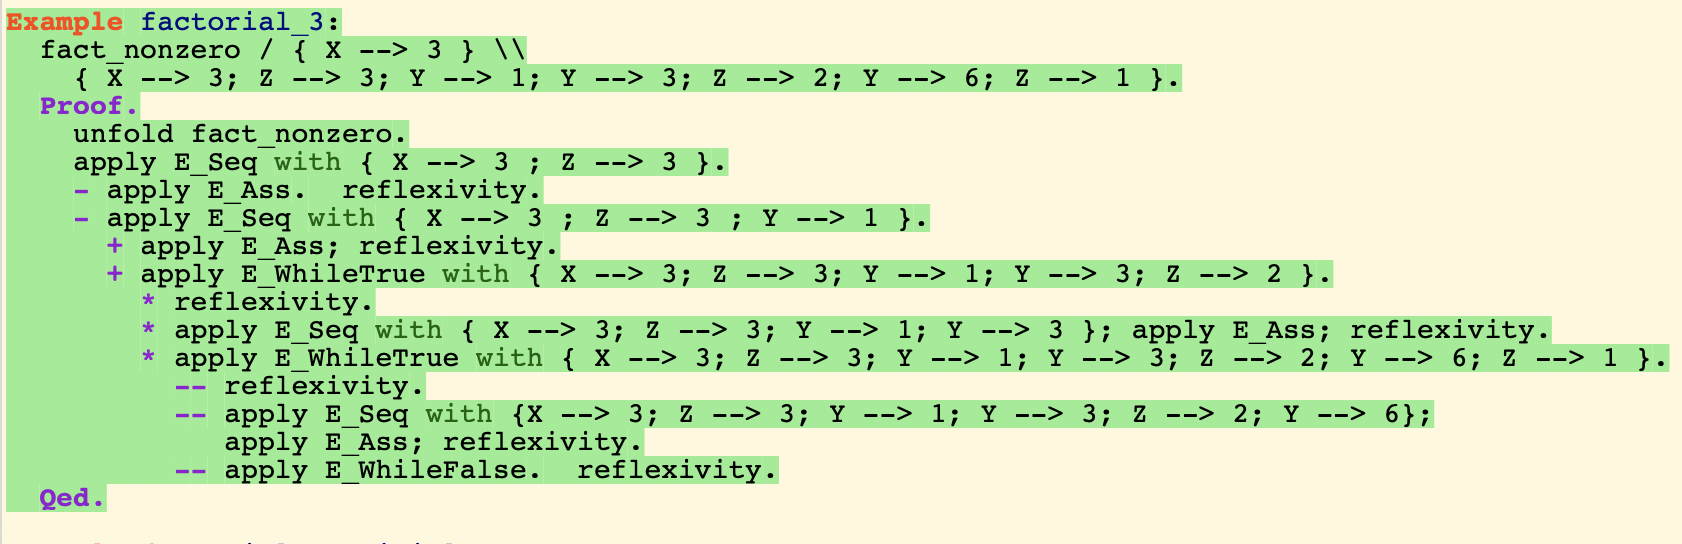
\includegraphics[scale=0.5]{factorial_3}
        \caption{Coq proof of Example \ref{firstoff}.}
        \label{fig:firstoff}
        \end{figure}
        \par\noindent The goal is initially
        \begin{verbatim}fact_nonzero / {X --> 3} \\
  {X --> 3; Z --> 3; Y --> 1; Y --> 3; Z --> 2; Y --> 6; Z --> 1}\end{verbatim}
        After unfolding the definition of \verb$fact_nonzero$, we use the tactic \verb$apply$ to invoke the definition of \verb$E_Seq$ from Definition \ref{commeval}, namely that
        \begin{verbatim}
c1 / st  \\ st’ -> c2 / st’ \\ st’’ -> (c1 ;; c2) / st \\ st’’. \end{verbatim}
       Since Coq cannot automatically infer what the intermediate state should be, we also supply it \verb$with { X --> 3 ; Z --> 3 }$.  This changes the goal into two subgoals
       \begin{verbatim}
______________________________________(1/2)
(Z ::= X) / {X --> 3} \\ {X --> 3; Z --> 3}
______________________________________(2/2)
(Y ::= 1;;
 WHILE ! (Z <= 1) DO Y ::= Y * Z;; Z ::= Z - 1 END) /
{X --> 3; Z --> 3} \\
{X --> 3; Z --> 3; Y --> 1; Y --> 3; Z --> 2; Y --> 6;
Z --> 1}
       \end{verbatim}
       Focusing on the first subgoal, we again use \verb$apply$ on \verb$E_Ass$, again from Definition \ref{commeval}.  Now we need to prove that 
       \verb$aeval {X --> 3} X = 3$, but as this is true from the definition of \verb$aeval$ (Definition \ref{aritheval}), it suffices to use \verb$reflexivity$ to dispatch the goal.
       \par The rest of the proof continues similarly.  At each step, there is really only one thing that can be done, and in fact it is quite mechanical.  We will point out, however, that each instance of \verb$E_WhileTrue$ runs through one iteration of the commands inside the while loop, and can only terminate by an application of \verb$E_WhileFalse$, i.e.\ a point where the guard condition is no longer true and we can exit the loop.
    \end{proof}
\end{example}

    For this section, we'll use as our running example the simple opaque predicate introduced in Chapter \ref{intro}, namely,
    \[
    	\forall x.\ (x * x + x + x + 1) = (x + 1) * (x + 1).
    \]
\begin{defin}
    We now define an opaque predicate transformation with our running example.  
    For the purposes of making the proofs easier to work with, and also to add a slight additional touch of obfuscation, we split up these assignments over multiple lines, as follows.
\begin{verbatim}
Definition opaque_trans x c1 c2 :=
  X' ::= (ANum x) ;;
  Z' ::= X' * X' ;;
  Z' ::= Z' + X' ;;
  Z' ::= Z' + X' ;;
  Z' ::= Z' + 1 ;;
  Z'' ::= X' + 1 ;;
  Z'' ::= Z'' * Z'' ;;
  IFB (BEq Z' Z'') THEN c1 ELSE c2 FI.
\end{verbatim}
That is, the \verb$opaque_trans$ function takes as input a number $x$ and programs $c_1$ and $c_2$, and returns the new program that executes $c_1$ if the equation
\[
	(x * x + x + x + 1) = (x + 1) * (x + 1)
\]
holds and executes $c_2$ otherwise.  Of course, the above is true for all $x$, so the resulting program should be the same as $c_1$.  We'd like to claim that a program transformed by \verb$opaque_trans$ is equivalent to the original.

\par The observant logically inclined reader should, at this point, now be suspicious about taking this claim at face value.  What do we mean when we say the transformed program should be ``the same''?  The next example, which shows what happens when $opaque\_trans$ is applied to the $factorial\_3$ example, elucidates the necessity to be precise.  First, however, we will need a few lemmas that show our opaque predicate is indeed such, in various incarnations to be used in proofs.
\end{defin}

\begin{lem}\label{opaqueness}
    It is indeed the case that for all $x\in \N$,\[
	(x * x + x + x + 1) = (x + 1) * (x + 1).
    \] 
    In Coq, this is actually the following four lemmas.
    \begin{enumerate}
        \item\label{opaqueA} \begin{verbatim}Lemma opaque_taut : forall x : nat, 
  x * x + x + x + 1 = (x + 1) * (x + 1).\end{verbatim}
        \item\label{opaqueB} \begin{verbatim}Lemma opaque_taut' : forall x : nat, 
  beq_nat (x * x + x + x + 1) ((x + 1) * (x + 1)) = true.\end{verbatim}
        \item\label{opaqueC} \begin{verbatim}Lemma opaque_taut_sym : forall x : nat, 
  (x + 1) * (x + 1) = x * x + x + x + 1.\end{verbatim}
        \item\label{opaqueD} \begin{verbatim}Lemma opaque_taut'_sym : forall x : nat, 
  beq_nat ((x + 1) * (x + 1)) (x * x + x + x + 1) = true.\end{verbatim}
    \end{enumerate}
    \begin{proof}
    \begin{enumerate}
        \item 
        The first lemma states the equation in terms of absolute equality of the natural number expressions.  After instantiating with \verb$intros x$, the goal is
        \[
            x * x + x + x + 1 = (x + 1) * (x + 1).
        \]
        Next, we apply \verb$rewrite -> mult_plus_distr_l$.  Here, \verb$rewrite$ tells Coq to rewrite the goal by applying an existing fact about equality, namely that multiplication left-distributes over addition, which is proven in Coq's default \verb$Nat$ library; this is the statement that \begin{verbatim}forall n m p : nat, n * (m + p) = n * m + n * p.\end{verbatim}
        The forwards arrow (in the tactic \texttt{rewrite -> mult\_plus\_distr\_l}) tells Coq to do the rewrite from left to right; that is, replace any instance of $n * (m + p)$ with $n * m + n * p$.  This changes our goal now to
        \[
            x * x + x + x + 1 = (x + 1) * x + (x + 1) * 1.
        \]
        Then, we apply \verb$rewrite -> mult_plus_distr_r$, which is analogous to the above for invoking the fact that multiplication is right-distributive over addition.  The goal now becomes 
        \[
            x * x + x + x + 1 = x * x + 1 * x + (x + 1) * 1.
        \]
        Finally, we conclude this proof with the \verb$omega$\index{omega} tactic, which solves goals in \define{Presburger arithmetic}.  In particular, this can handle rewrites over linear arithmetic, which are now the only differences remaining between the left and right sides of the goal.
        \item
        This is the ``same" statement as before, but expressed in terms of \verb$beq_nat$, which is a function of type \verb$nat -> nat -> bool$.  It takes two values of type \verb$nat$ and returns a \verb$bool$ value that represents whether the two expressions of type $\N$ are equal.  This is necessary because of the way evaluation of IMP programs has been defined, as it allows us to use variables to condition on the truth of a boolean expression involving natural numbers.  
        \par The proof is straightforward, as there is an existing lemma \verb$beq_nat_true_iff$ from the Coq libraries that allow us to pass between the two forms.  The proof in Coq is just
        \begin{verbatim}intro x.  rewrite beq_nat_true_iff.  apply opaque_taut.\end{verbatim}
        \item
        This is \eqref{opaqueA} with the equality in the opposite direction.  It's proven by
        \begin{verbatim}intro x.  symmetry.  apply opaque_taut.\end{verbatim}  The \verb$symmetry$ tactic reverses the two sides of the equality in the goal, after which we apply the lemma from \eqref{opaqueA} to conclude the proof.  Proving the symmetric version is slightly more work now, but gives us the ability to apply whichever one is needed in future proofs.
        \item Similar to \eqref{opaqueC}, this is the symmetric version of \eqref{opaqueB}, and is proven by
        \begin{verbatim}intro x.  rewrite beq_nat_true_iff.  apply opaque_taut_sym.\end{verbatim}
    \end{enumerate}\qedhere
    \end{proof}
\end{lem}

\begin{example}\label{firstfact}
    For any $x\in \N$ and any program $c_2$, \verb$opaque_trans x fact_nonzero c2$ with input $X=3$ yields output $Y=6$.  In Coq, however, it looks as follows.
    \begin{verbatim}Example factorial_3_opaque_trans:
  forall x c2, opaque_trans x fact_nonzero c2 / { X --> 3 } \\
    { X --> 3; X' --> x; Z' --> x * x; Z' --> x * x + x; Z' --> x * x + x + x;
      Z' --> x * x + x + x + 1; Z'' --> x + 1; Z'' --> (x + 1) * (x + 1); 
      Z --> 3; Y --> 1; Y --> 3; Z --> 2; Y --> 6; Z --> 1 }.\end{verbatim}
      After instantiating variables and unfolding the definitions, the transformed program looks like
      \begin{verbatim}
X' ::= x;;
Z' ::= X' * X';;
Z' ::= Z' + X';;
Z' ::= Z' + X';;
Z' ::= Z' + 1;;
Z'' ::= X' + 1;;
Z'' ::= Z'' * Z'';;
IFB Z' = Z''
THEN Z ::= X;;
  Y ::= 1;;
  WHILE ! (Z <= 1) DO Y ::= Y * Z;; Z ::= Z - 1 END
ELSE c2 FI
      \end{verbatim}
      We omit explaining the proof here, which does not use any new ideas beyond the previous example, save for an instance of \verb$apply opaque_taut'$ to use Lemma \ref{opaqueness} when we reach the If statement.
\end{example}

Although we did prove that our opaque predicate transformation worked (that is, preserves the fact that if $X=n$ in the start state, then $Y=n!$ in the end state) on our simple factorial program with the generality of any numerical value for the opaque predicate and any dummy program, it seems that there is no direct way to generalize this into a more general theorem.  What we would have liked to state was that if a program took a state $st$ to a state $st'$, then its transformed version would also take $st$ to $st'$.  Unfortunately, our transformation introduces new variables, which affects the value of the end state, even if those variables are not of interest to us.

\par We cannot use \verb$cequiv$ \eqref{commequiv} --- that is, we can't use it with the current formulation of the transformation) --- since new variables and assignments are introduced and kept track of in the definition of the state, even if we ultimately don't care about them.  
\par Thus we were not ultimately successful, in this initial approach, in formulating a statement with command equivalence (\ref{commequiv}).  We'll revisit this in Section \ref{noass}.

\section{Hoare logic equivalence}\label{hoarequiv}

In this section, we explore using Hoare logic to specify program conditions, and then generalize the result as much as we can.  The main idea with Hoare logic is that we can be more specific about what we wish a transformation to preserve (in our case, just the value of a single variable before the program runs and the value of a single variable after the program finishes, rather than the entire state as in the previous section).  First, we'll use a slightly different formulation of the factorial program.

\begin{defin}[Factorial program (count-up formulation)]\index{factorial program!count-up formulation}
This version of the factorial program counts up from zero rather than down from $X$, and works for input $0$ as well.
\begin{verbatim}
Definition fact_program : com :=
  Y ::= 1;;
  Z ::= 0;;
  WHILE ! (Z = X) DO
    Z ::= Z + 1;;
    Y ::= Y * Z
  END.
\end{verbatim}
\end{defin}

We begin by restating Example \ref{firstoff}, replacing the specific values of $3$ and $6$ with arbitrary natural numbers, as the Hoare triple
\[
    (| X = x_0 |)\ fact\_program\ (| Y = x_0! |).
\]

We give definitions of the assertions on the values of $X$ and $Y$ in Coq as follows.

\begin{verbatim}
Definition as_x (x0 : nat) : Assertion := (fun st => st X = x0).
Definition as_y (y0 : nat) : Assertion := (fun st => st Y = y0).
\end{verbatim}

Before we continue with our formulation and proof of Hoare logic equivalence, we need a lemma about a fundamental property of factorial that we usually take for granted.  The proof is worth discussing, as it invokes several tactics we've not yet used.

    First, in Coq, the definition of the factorial\footnote{This factorial function is built-in at the level of Coq itself.  The factorial program \texttt{fact\_program} we defined is an IMP program, which is the imperative programming language defined inside of Coq that we are using to reason about program execution.}, which one can check with the command \verb$Print fact$, is the recursive function
    \begin{verbatim}
fact = 
fix fact (n : nat) : nat :=
  match n with
  | 0 => 1
  | S n0 => S n0 * fact n0
  end
     : nat -> nat.\end{verbatim}
    \par \indent We remark that while it would be theoretically possible to do obfuscation proofs in Coq's functional language directly, the choice of IMP is for its minimalism and simplicity --- we wish to cleave to the matter and focus on certifying obfuscating transformations without getting bogged down by any unnecessary complexities of the language.

\begin{lem}\label{factdist}
    For all $x \in \N$, $x! \times (x + 1) = (x + 1)!$.  The statement in Coq is
    \begin{verbatim}Lemma fact_dist : forall x : nat, fact x * (x + 1) = fact (x + 1).\end{verbatim}
    \begin{proof}
     A screenshot of the proof is below.
    
    \noinden        \begin{figure}[H]
        \centering
        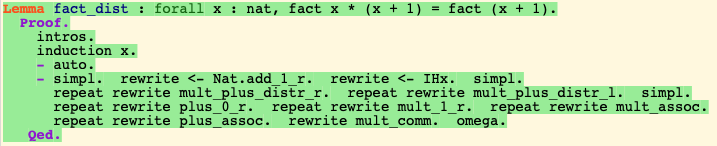
\includegraphics[scale=0.6]{fact_dist}
        \caption{Coq proof of Lemma \ref{factdist}.}
        \label{fig:firstoff}
        \end{figure}
    \par The tactic \verb$intros$\index{intros} will instantiate as many variables or conditional hypotheses as immediately useful, with Coq assigning names automatically if they're not supplied.  In this case, it's just the single variable \verb$x : nat$, which leaves us with the goal
    \[
\mathtt{fact\ x * (x + 1) = fact\ (x + 1)}.
    \]
    Now, $x$ is an arbitrary natural number, so we proceed by \define{induction}.  The natural number type has two constructors, one which declares the constant $0$, and the successor function $S: \N \to \N$.  Thus using the tactic \verb$induction x$ breaks it into the following subgoals, which correspond to the notions of \define{base case} and \define{inductive case} of familiar informal induction proofs over the natural numbers.
    \begin{equation}\label{factindzero}
    \texttt{fact 0 * (0 + 1) = fact (0 + 1)}
    \end{equation}
    \begin{equation}\label{factindind}
    \texttt{fact (S x) * (S x + 1) = fact (S x + 1)}
    \end{equation}
    The base case \eqref{factindzero} is ``immediately obvious", even to Coq, and so can be solved with \verb$auto$\index{auto}.  In this case, it's a direct application of the definitions, but it is in fact quite powerful.  Intuitively, one can attempt to use it whenever the goal seems ``easy" or ``obvious" and/or one is feeling lazy; however, it is obviously best to avoid overusing it when teaching, learning, or explaining things in detail.  As an aside, it can even in one application solve \define{modus tollens} (i.e.\ the statement $\forall P,Q\in Prop, (P \to Q) \implies (\neg Q \to \neg P)$).  However, it was \emph{not} able to handle the statement of this lemma, which the author attempted when faced with an instance of it, prompting the need to go back and prove it explicitly.
    \par Next, we focus the proof on the inductive goal \eqref{factindind}.  When we do, we are given the inductive hypothesis to work with,
    \begin{equation}\label{hypind}
\texttt{IHx\ :\ fact\ x * (x + 1) = fact\ (x + 1)}
    \end{equation}
    The first tactic we use is \verb$simpl$, which attempts to simplify expressions.  In this case, Coq does what it can with the definitions of \verb$fact$ and $S$, changing the goal from \eqref{factindind} to
    \begin{equation*}
\texttt{(fact x + x * fact x) * S (x + 1) =
fact (x + 1) + (x + 1) * fact (x + 1)}.
    \end{equation*}
    The rest of the proof is not particularly interesting and so we will gloss over the details.  They are essentially a sequence of rewrites using existing facts in the Coq libraries about natural numbers, addition, and multiplication, more uses of \verb$simpl$, a rewrite with the induction hypothesis \eqref{hypind}, and a final use of \verb$omega$ to dispatch the remaining math.  The tactic \verb$repeat$\index{repeat} is a \define{tactical}, or higher-order tactic, which takes another tactic as an argument.  It will, as the name suggests, repeatedly apply that tactic until it no longer has any effect.
    \end{proof}
\end{lem}
\begin{rem}
Sequences of rewrites such as those in the preceding lemma to solve mathematical goals are certainly not canonical, and there may be multiple other ways to do it.  The process of choosing which rewrites and tactics to use involves staring at the two sides of the equation, thinking about how to get them to be the same, and then applying a combination of intuition and trial-and-error.  
    \par In fact, the proof was originally lengthier and more awkward than what is currently presented, until the present author starting writing up this explanation.  In desiring to save both himself and the reader some mind-numbing tedium, he found ways to shorten the proof and make it more elegant.
    \end{rem}
    
Recall that Coq allows the user to define custom tactics\index{custom tactic} to handle repetitive and mechanical parts of proofs.  These can get quite advanced, but we create just a simple one applying three individual tactics in a row, which will be used many times in the proofs to come.
\index{Ltac}
\begin{verbatim}
Ltac disp := simpl; unfold assert_implies; auto.
\end{verbatim}

This tactic, which we simply named \verb$disp$, short for ``dispatch"\index{dispatch}, attempts to first use \verb$simpl$ on the goal, then unfold the definition of \verb$assert_implies$ \eqref{assertimplies}, and finish off with the almighty \verb$auto$ hammer.

\begin{example}\label{hoareexample1}
    We are now ready to prove
    \[
     (|X=x_0|)\ fact\_program\ (|Y=x_0!|)
    \]
    which in Coq is
    \begin{verbatim}
Example factorial_all_hoare: forall xo,
  {{ as_x xo }} fact_program {{ as_y (fact xo) }}.\end{verbatim}
    \begin{proof}
    A screenshot of the proof is below.
    
    \noindent        \begin{figure}[H]
        \centering
        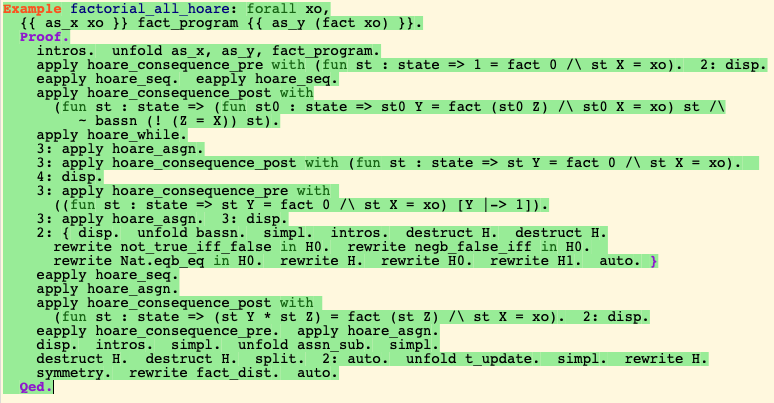
\includegraphics[scale=0.6]{fact_hoare1}
        \caption{Coq proof of Example \ref{hoareexample1}.}
        \label{fig:hoareexample1}
        \end{figure}
    \par After the first line of \verb$intros$ and \verb$unfold$s, we have an instantiated \verb$xo : nat$ and Hoare triple goal of
    \begin{verbatim}
{{fun st : state => st X = xo}}
Y ::= 1;;
Z ::= 0;;
WHILE ! (Z = X)
DO Z ::= Z + 1;; Y ::= Y * Z END
{{fun st : state => st Y = fact xo}}\end{verbatim}
    Due to the exactness of form required by the Hoare logic rules as they step through the program, the first thing we need to do is massage the pre-condition by replacing $X = x_0$ with the equivalent (although we could use something strictly stronger) pre-condition $(1 = 0!) \land (X = x_0)$.  After \verb$apply hoare_consequence_pre$ \eqref{hoareconsequence} with the appropriate assertion, we now have two goals.
    \begin{verbatim}
______________________________________(1/2)
{{fun st : state => 1 = fact 0 /\ st X = xo}}
Y ::= 1;;
Z ::= 0;;
WHILE ! (Z = X)
DO Z ::= Z + 1;; Y ::= Y * Z END
{{fun st : state => st Y = fact xo}}
______________________________________(2/2)
(fun st : state => st X = xo) ->>
(fun st : state => 1 = fact 0 /\ st X = xo)
    \end{verbatim}
    The second goal is to prove that our new pre-condition is indeed implied by the original one.  By using \verb$2: disp$, we are telling Coq first to focus on the second subgoal, and use our previously defined \verb$disp$ custom tactic, which succeeds in solving it.
    \par Returning to the first goal, we observe the program part of the Hoare triple is a sequence of three commands, so we need to use the corresponding rule \eqref{hoareseq} twice.  The tactic used is \verb$eapply hoare_seq$; here, \verb$eapply$ is similar to \verb$apply$, except we do not supply the intermediate state, telling Coq ``leave it for now, it'll soon be clear what it should be."  This turns the first goal above into the following three goals, where \verb$?Q$ and \verb$?Q0$ are the momentarily unknown middle states.
    \begin{verbatim}
______________________________________(1/3)
{{?Q0}} WHILE ! (Z = X) DO Z ::= Z + 1;; Y ::= Y * Z END
{{fun st : state => st Y = fact xo}}
______________________________________(2/3)
{{?Q}} Z ::= 0 {{?Q0}}
______________________________________(3/3)
{{fun st : state => 1 = fact 0 /\ st X = xo}} Y ::= 1 {{?Q}}
    \end{verbatim}
 
    Next, we use \eqref{hoareconsequence} again, this time \verb$apply hoare_consequence_post$, to weaken the post-condition to the exact form that the while loop will terminate on.  Note here the introduction of the loop invariant, $!(Z=X)$; this statement remains true for each iteration of the while loop until it terminates, when the counter variable has reached the value of the input.  
    \par As far as doing these types of proofs informally on paper before formalizing them in Coq, this is really the only non-mechanical part that requires (possibly) non-trivial insight; the assignment/skip/if rules are all straightforward, and while we do need to come up with some assertions in the pre- and post-condition massaging, it usually becomes evident what they need to be by working through the intermediary commands.
    \par
    Our goals are now the following.
\begin{verbatim}
{{?Q0}} WHILE ! (Z = X) DO Z ::= Z + 1;; Y ::= Y * Z END
{{fun st : state => (st Y = fact (st Z) /\ st X = xo) /\ 
  ~ bassn (! (Z = X)) st}}
______________________________________(2/4)
(fun st : state => (st Y = fact (st Z) /\ st X = xo) /\ 
  ~ bassn (! (Z = X)) st) ->>
(fun st : state => st Y = fact xo)
______________________________________(3/4)
{{?Q}} Z ::= 0 {{?Q0}}
______________________________________(4/4)
{{fun st : state => 1 = fact 0 /\ st X = xo}} Y ::= 1 {{?Q}}
\end{verbatim}
Now, we \verb$apply hoare_while$ \eqref{hoarewhile}.  Due to the form this rule takes, Coq knows exactly what \verb$Q0$ has to be, thus changing the first and third goal from the above to the following (we omit repeating the goals that haven't changed).
\begin{verbatim}
______________________________________(1/4)
{{fun st : state => (st Y = fact (st Z) /\ st X = xo) /\ bassn (! (Z = X)) st}}
Z ::= Z + 1;; Y ::= Y * Z {{fun st : state => st Y = fact (st Z) /\ st X = xo}}
______________________________________(3/4)
{{?Q}} Z ::= 0 {{fun st : state => st Y = fact (st Z) /\ st X = xo}}
\end{verbatim}
Now that the post-condition in the third goal is known, we can use \verb$3: apply hoare_asgn$ \eqref{hoareassign}, which fills in what \verb$Q $is, just as we did with \verb$Q0$ before.  This solves the third goal above, now the fourth goal from before with \verb$Q $is now
\begin{verbatim}
______________________________________(3/3)
{{fun st : state => 1 = fact 0 /\ st X = xo}} Y ::= 1
{{(fun st : state => st Y = fact (st Z) /\ st X = xo) [Z |-> 0]}}
\end{verbatim}
We skip explaining the next few lines, which are just some more applications of the consequence rules and our dispatch tactic, and pick up from after \verb$3: disp$, whence our goals are
\begin{verbatim}
______________________________________(1/2)
{{fun st : state => (st Y = fact (st Z) /\ st X = xo) /\ bassn (! (Z = X)) st}}
Z ::= Z + 1;; Y ::= Y * Z {{fun st : state => st Y = fact (st Z) /\ st X = xo}}
______________________________________(2/2)
(fun st : state => (st Y = fact (st Z) /\ st X = xo) /\ ~ bassn (! (Z = X)) st) 
  ->> (fun st : state => st Y = fact xo)
\end{verbatim}
We focus on the second goal and apply \verb$disp$, which makes some progress but leaves us with
\begin{verbatim}
forall st : state, (st Y = fact (st Z) /\ st X = xo) /\
  ~ bassn (! (Z = X)) st -> st Y = fact xo
\end{verbatim}
We use \verb$unfold bassn$ followed by \verb$simpl$, leaving the goal at 
\begin{verbatim}
forall st : state, (st Y = fact (st Z) /\ st X = xo) /\
  negb (st Z =? st X) <> true -> st Y = fact xo
\end{verbatim}
This goal has both a universal quantifier and then a conditional statement, so we use \verb$intros$ to introduce both as hypotheses, giving us the following (where above the line, \verb$st$ and \verb$H $are the newly instantiated items).
\begin{verbatim}
xo : nat
st : state
H : (st Y = fact (st Z) /\ st X = xo) /\
    negb (st Z =? st X) <> true
______________________________________(1/1)
st Y = fact xo
\end{verbatim}
We now meet \verb$destruct$\index{destruct} for the first time, which breaks down inductive types into their possible components.  We apply it twice on \verb$H $to break apart the conjuncts in the hypotheses.
\begin{verbatim}
xo : nat
st : state
H : st Y = fact (st Z)
H1 : st X = xo
H0 : negb (st Z =? st X) <> true
______________________________________(1/1)
st Y = fact xo
\end{verbatim}
Next, we apply several rewrites in \verb$H0$ of known facts, changing it ultimately to \verb$H0 : st Z = st X$.  Then, a few rewrites with our hypotheses solves the current goal.
\par We'll skip ahead a few more lines again, until the next tactic we haven't seen before shows up near the end of the proof, and pick up after the two uses of \verb$destruct H$ on the second last line.  At this stage, the hypotheses and goals are
\begin{verbatim}
xo : nat
st : state
H : st Y = fact (st Z)
H1 : st X = xo
H0 : bassn (! (Z = X)) st
______________________________________(1/1)
(st & {Z --> st Z + 1}) Y * (st & {Z --> st Z + 1}) Z =
fact ((st & {Z --> st Z + 1}) Z) /\
(st & {Z --> st Z + 1}) X = xo
\end{verbatim}
Before, we used \verb$destruct$ to break apart a conjunction in a hypothesis, but here we have a conjunction in a goal, which can be \verb$split$\index{split}, changing the goals to
\begin{verbatim}
______________________________________(1/2)
(st & {Z --> st Z + 1}) Y *
(st & {Z --> st Z + 1}) Z =
fact ((st & {Z --> st Z + 1}) Z)
______________________________________(2/2)
(st & {Z --> st Z + 1}) X = xo
\end{verbatim}
The second goal can be solved with a simple \verb$2: auto$ (note that \verb$H1$ already says \verb$st X = xo$, and clearly doing something to a different variable won't change that).  To proceed with the first goal, we \verb$unfold t_update$ (Section \ref{Maps}) to yield
\begin{verbatim}
(if beq_string Z Y then st Z + 1 else st Y) *
(if beq_string Z Z then st Z + 1 else st Z) =
fact (if beq_string Z Z then st Z + 1 else st Z).
\end{verbatim}
These string equality checks are easily \verb$simpl$ified to
\begin{verbatim}
st Y * (st Z + 1) = fact (st Z + 1).
\end{verbatim}
A \verb$rewrite H$ and \verb$symmetry$ gets us to
\begin{verbatim}
fact (st Z + 1) = fact (st Z) * (st Z + 1)
\end{verbatim}
which is then solved by applying Lemma \ref{factdist}.
\end{proof}
\end{example}

We have proven that when $X = x_0$ before the (unobfuscated) \texttt{fact\_program} runs, then $Y = x_0!$ after the fact.  We now turn to showing that when we obfuscate $\texttt{fact\_program}$, it remains the case that $X = x_0$ beforehand implies $Y = x_0!$ when the program finishes.

\par

In the following, we use a new formulation of the opaque predicate transformation, as it now makes our life easier to collapse the assignments into single lines.

\begin{verbatim}
Definition opaque_trans' x c1 c2 :=
  X' ::= (ANum x) ;;
  Z' ::= X' * X' + X' + X' + 1 ;;
  Z'' ::= (X' + 1) * (X' + 1) ;;
  IFB (BEq Z' Z'') THEN c1 ELSE c2 FI.
\end{verbatim}

\begin{example}\label{hoarel2}
    We now prove the same Hoare triple holds with the obfuscated factorial program in place of the original program.
    \[
     \forall x_0 \in \N,\ \forall c_2 \in Com, (|X=x_0|)\ opaque\_trans'\ (X, fact\_program, c_2)\ (|Y=x_0!|)
    \]
    which in Coq is
    \begin{verbatim}
Example factorial_all_hoare_opaque: forall x xo c2,
  {{ as_x xo }} (opaque_trans' x fact_program c2) {{ as_y (fact xo) }}.\end{verbatim}
\begin{proof}
As we can see in the screenshot of the proof, we have added comments for readability, separating the proof into three parts.

        \begin{figure}[H]
        \centering
        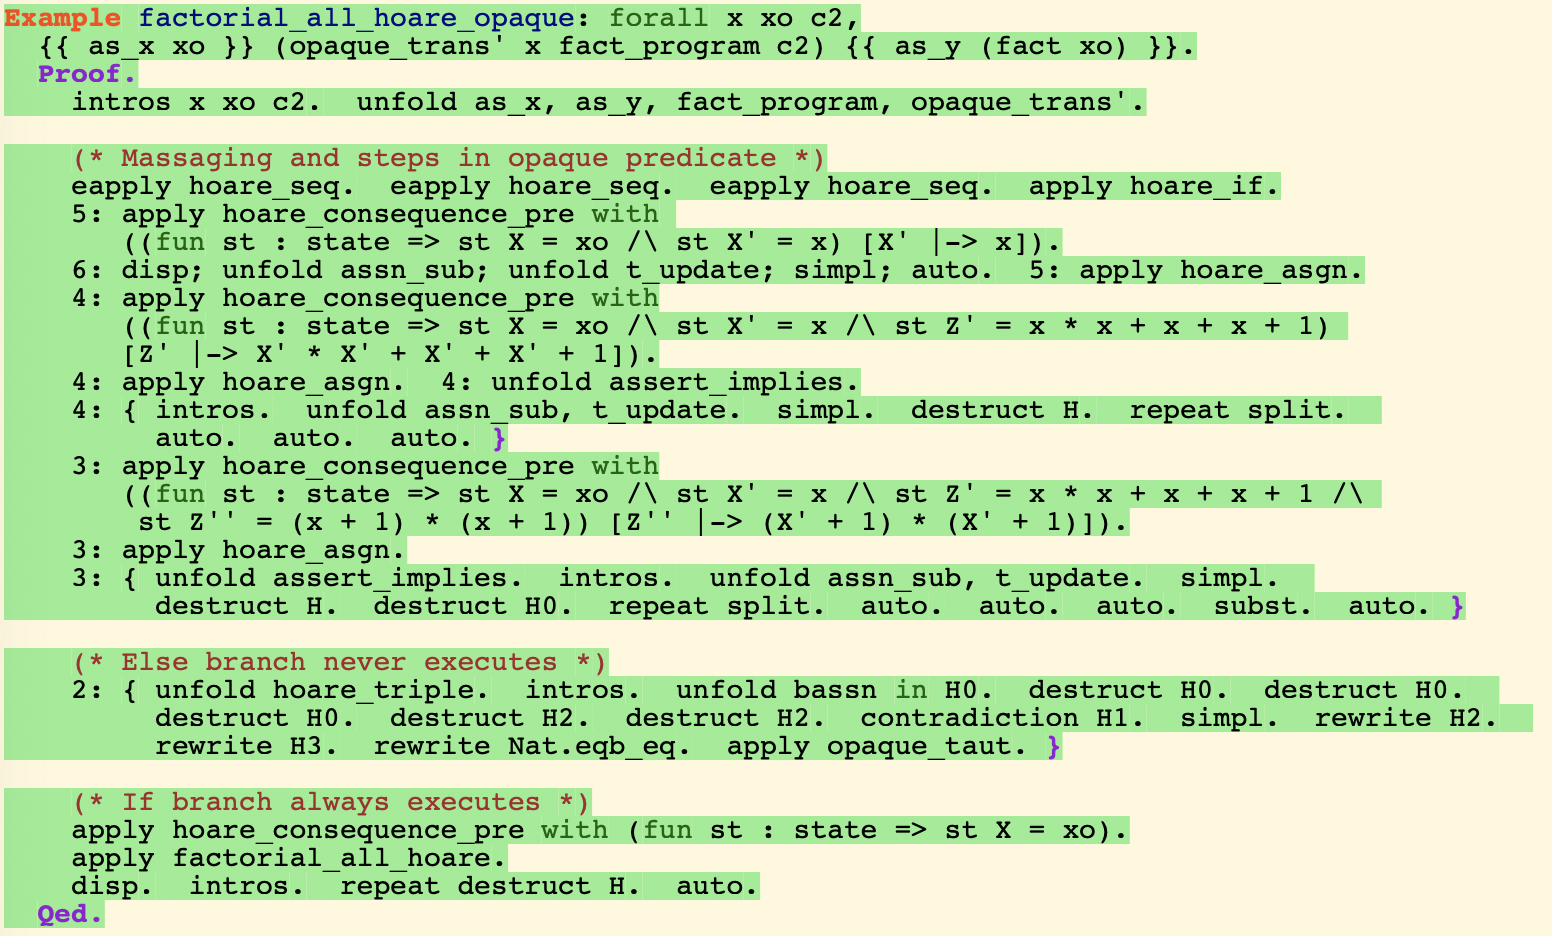
\includegraphics[scale=0.6]{hoare_opaque}
        \caption{Coq proof of Example \ref{hoarel2}.}
        \label{fig:hoare12}
        \end{figure}

The following is the proof state after first line of intros and unfolds, which shows the transformed program.

\begin{verbatim}
1 subgoal
x, xo : nat
c2 : com
______________________________________(1/1)
{{fun st : state => st X = xo}}
X' ::= x;;
Z' ::= X' * X' + X' + X' + 1;;
Z'' ::= (X' + 1) * (X' + 1);;
IFB Z' = Z''
THEN Y ::= 1;;
     Z ::= 0;;
     WHILE ! (Z = X) DO Z ::= Z + 1;; Y ::= Y * Z
     END ELSE c2 FI
{{fun st : state => st Y = fact xo}}\end{verbatim}

We'll skip over the ``massaging and steps in opaque predicate" part, which goes through the first few lines of assignment and pre- and post-condition massaging, and doesn't use any tactics or bright ideas we haven't seen already.  At the end of this section of the proof, we have dealt with the assignments introduced by the opaque predicate transformation, and it remains to solve what was invoked by \verb$apply hoare_if$.
\begin{verbatim}
2 subgoals
x, xo : nat
c2 : com
______________________________________(1/2)
{{fun st : state =>
  (fun st0 : state =>
   st0 X = xo /\
   st0 X' = x /\
   st0 Z' = x * x + x + x + 1 /\
   st0 Z'' = (x + 1) * (x + 1)) st /\
  bassn (Z' = Z'') st}}
Y ::= 1;;
Z ::= 0;;
WHILE ! (Z = X) DO Z ::= Z + 1;; Y ::= Y * Z END
{{fun st : state => st Y = fact xo}}
______________________________________(2/2)
{{fun st : state =>
  (fun st0 : state =>
   st0 X = xo /\
   st0 X' = x /\
   st0 Z' = x * x + x + x + 1 /\
   st0 Z'' = (x + 1) * (x + 1)) st /\
  ~ bassn (Z' = Z'') st}} c2
{{fun st : state => st Y = fact xo}}
\end{verbatim}
The first subgoal corresponds to the if-then branch (when the opaque predicate evaluates to true, which is always), and the second to the if-else branch (when the opaque predicate evaluates to false, which is never).  We'll first focus on the latter.  After the initial \verb$intros$ and two \verb$unfold$s, we are in this proof state.
\begin{verbatim}
x, xo : nat
c2 : com
st, st' : state
H : c2 / st \\ st'
H0 : (st X = xo /\
      st X' = x /\
      st Z' = x * x + x + x + 1 /\
      st Z'' = (x + 1) * (x + 1)) /\
     beval st (Z' = Z'') <> true
______________________________________(1/1)
st' Y = fact xo
\end{verbatim}
Next, we have five \verb$destruct$s to fully separate \verb$H0$.
\begin{verbatim}
1 subgoal
x : nat
c2 : com
st, st' : state
H : c2 / st \\ st'
H0 : st X' = x
H2 : st Z' = x * x + x + x + 1
H3 : st Z'' = (x + 1) * (x + 1)
H1 : beval st (Z' = Z'') <> true
______________________________________(1/1)
st' Y = fact (st X)
\end{verbatim}
Now, \verb$H1$ is false by construction regardless of what parameters were passed to the opaque predicate transformation, so we use \verb$contradiction H1$ to invoke \define{reductio ad absurdum} --- if we can prove that something that becomes a hypothesis after entering this branch is false, then it must be the case that this can never happen.  Our original goal is replaced by the negation of \verb$H1$.
\begin{verbatim}
______________________________________(1/1)
beval st (Z' = Z'') = true
\end{verbatim}
After some \verb$simpl$ification and \verb$rewrite$s, the goal is
\begin{verbatim}
______________________________________(1/1)
x * x + x + x + 1 = (x + 1) * (x + 1)
\end{verbatim}
which we close with \verb$apply opaque_taut$ (Lemma \ref{opaqueness}\eqref{opaqueA}).
\par Now all that remains is proving that when we do enter the if-then branch, the remainder of the program executes as specified.  The goal is
\begin{verbatim}
______________________________________(1/1)
{{fun st : state =>
  (fun st0 : state =>
   st0 X = xo /\
   st0 X' = x /\
   st0 Z' = x * x + x + x + 1 /\
   st0 Z'' = (x + 1) * (x + 1)) st /\
  bassn (Z' = Z'') st}}
Y ::= 1;;
Z ::= 0;;
WHILE ! (Z = X) DO Z ::= Z + 1;; Y ::= Y * Z END
{{fun st : state => st Y = fact xo}}.
\end{verbatim}
After one more \verb$apply hoare_consequence_pre$, we are left with
\begin{verbatim}
______________________________________(1/2)
{{fun st : state => st X = xo}}
Y ::= 1;;
Z ::= 0;;
WHILE ! (Z = X) DO Z ::= Z + 1;; Y ::= Y * Z END
{{fun st : state => st Y = fact xo}}
______________________________________(2/2)
(fun st : state =>
 (st X = xo /\
  st X' = x /\
  st Z' = x * x + x + x + 1 /\
  st Z'' = (x + 1) * (x + 1)) /\
 bassn (Z' = Z'') st) ->>
(fun st : state => st X = xo).
\end{verbatim}
The first goal is now exactly the same as Example \ref{hoareexample1}, so we can simply use the entire previous example here with \verb$apply factorial_all_hoare$.  The second goal is just leftover bureaucracy that needs to be proven from \verb$hoare_consequence_pre$, which is handled with a few straightforward tactics.
\end{proof}
\end{example}

We've now successfully shown that our factorial program, both with and without the opaque predicate transformation, satisfies a Hoare triple of the form
\[ (| X = x_0 |)\ c\ (| Y = y_0 |), \]
and we would like to generalize\footnote{Our result is still rather specific; the only pre-condition we treat is that a specific variable $X$ takes on some value, and the only post-condition we treat is that a specific variable $Y$ takes on some value.  The pre- and post- conditions in Hoare logic could be more general, such as assertions that a variable isn't equal to some value, is greater than some value, or a conjunction or disjunction of several other statements.}.  Let's introduce a new term: \define{Hoare fidelity}.

\begin{defin}[Hoare fidelity (with respect to input X and output Y)]
A program $c_2$ preserves the Hoare fidelity of a program $c_1$ with respect to input X and output Y, if the validity of the Hoare triple
\[
(| X = x_0 |)\ c_1\ (| Y = y_0 |)
\]
implies the validity of the Hoare triple
\[
(| X = x_0 |)\ c_2\ (| Y = y_0 |).
\]
In Coq,
\begin{verbatim}
Definition Hoare_fidelity_xy c1 c2 := forall xo yo,
  hoare_triple (as_x xo) c1 (as_y yo) -> hoare_triple (as_x xo) c2 (as_y yo).\end{verbatim}
\end{defin}

Indeed, the decision to use the factorial program in the previous examples for illustrative purposes was an unnecessary detail, so we replace it with an arbitrary program.

\begin{theo}\label{hoare_xy_main}
For all programs $c_1$ and $c_2$, and all $x \in \N$, the transformed program $opaque\_trans'(x, c_1, c_2)$ preserves the Hoare fidelity with respect to input X and output Y of $c_1$.  In Coq, \begin{verbatim}
Theorem Opaque_trans_hoare_fidelity_xy : forall x c1 c2,
  Hoare_fidelity_xy c1 (opaque_trans' x c1 c2).
\end{verbatim}
\begin{proof}
    The proof is a direct generalization of Example \ref{hoarel2} with minor changes to reflect the fact that we're using an arbitrary program.
    
    \noindent         \begin{figure}[H]
        \centering
        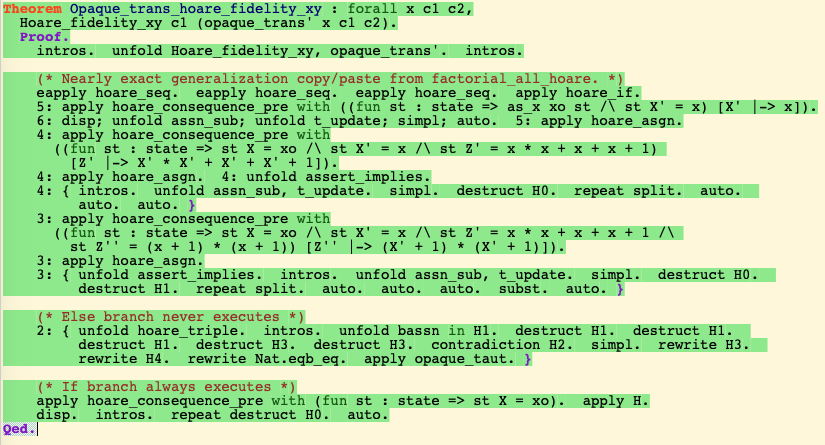
\includegraphics[scale=0.5]{hoare_xy_main}
        \caption{Coq proof of Theorem \ref{hoare_xy_main}.}
        \label{fig:hoare_xy_main}
        \end{figure}
\end{proof}
\end{theo}
This is more general, but still somewhat arbitrary.  The choice to have $X=x_0$ and $Y=y_0$ as pre- and post-conditions to consider was a result of the particular program we started with.  So let's attempt to generalize this further\footnote{We've generalized to the point that the specific program no longer matters, but we are still requiring a specific subset of possible pre- and post-conditions.} now.

\begin{defin}[Hoare fidelity (general)]
A program $c_2$ preserves the Hoare fidelity of a program $c_1$ with respect to pre-condition $P$ and post-condition $Q$, if the validity of the Hoare triple
\[
(| P |)\ c_1\ (| Q |)
\]
implies the validity of the Hoare triple
\[
(| P |)\ c_2\ (| Q |).
\]
In Coq,
\begin{verbatim}
Definition Hoare_fidelity c1 c2 P Q :=
  hoare_triple P c1 Q -> hoare_triple P c2 Q.
\end{verbatim}
\end{defin}

The corresponding theorem we'd like to prove now is the following.

\begin{nontheo}\label{hoarefail}
For all programs $c_1$ and $c_2$, all pre-conditions $P$ and post-conditions $Q$, and all $x \in \N$, the transformed program $opaque\_trans'(x, c_1, c_2)$ preserves the Hoare fidelity with respect to $P$ and $Q$ of $c_1$.
\begin{proof}
    Whoops.  This isn't even true.\footnote{The point of this ``non-theorem" is that we stated something that we initially thought was true, and upon initial reflection, seemed like it should be.  We then attempted to do the proof in Coq, but we were able to realize that there was an error in formulating the statement when we reached a point where the goal becomes something that is unprovable.}  We get as far as we can before realizing we can't continue, and close the proof with \verb$Abort$\index{abort}, which leaves the unfinished attempt in the script but lets us move on without finishing the proof\footnote{This means the theorem's proof isn't completed and isn't valid as far as Coq is concerned.  However, we may leave it in the script if there is some value to be gained from discussing what went wrong.  It may also be the case that a theorem \emph{is} valid, but we simply wish to leave it for the time being and come back later to finish it.}.
\end{proof}
\end{nontheo}

We momentarily leave it as an exercise to the reader to think about why this hasty generalization is faulty (the answer is in the comments in the code \cite{repo}).  We will run into the exact same problem later in Section \ref{flattenif} and provide a solution there.  
\par For now, we'll simply remark that this is \emph{precisely} one of the foremost practical benefits of going through the rigours of formal verification --- discovering something that ``sounds about right" actually isn't as-stated, and preventing a bug from ever seeing the light of day instead of fixing it after the fact (which could be too late, as discussed at the start of Chapter \ref{two}).

\section{A formulation without assignment}\label{noass}
In the first presentation of the opaque predicate transformation from Section \ref{naive}, we used a program that allowed
the user (that is, the person obfuscating the code) to specify a particular number, and then add a number of assignments before the
opaque predicate check, and then ultimately noted at the end of Section \ref{naive} that command equivalence (which depends on the full state --- that is, the equality of values of \emph{all} variables) did not
hold in this model due to these extra assignments and variables.
\par
We now present an alternate formulation with no assignments, with the entire predicate
built into the boolean condition of the branching statement. On the one hand, the entire
equation appears on a single line instead of a number of assignments, which may make it
easier to detect, but on the other hand, it can access any variable already being used (and
in the case of IMP, also any variable not already being used; recall a state in IMP is a total map
from strings to $\N$ and all variables have default value 0).  In this case, state equivalence can be proven in general.
\par
The point, ultimately, is that our transformations should be as modular as possible, and act on as small a piece of a possibly larger program as possible.  We'll start with some definitions of functions to make arbitrary opaque predicates.  We note that the code for this section was developed in collaboration with Bahman Sistany, the present author's supervisor (manager) during his co-op term at Irdeto where this research began. 

\begin{defin}[Make opaque predicate functions]
We define in Coq the following.
\begin{verbatim}
Definition make_opaque_pred (a1 a2: aexp): bexp := BEq a1 a2.
Definition make_opaque_pred_IFB b c1 c2 := IFB b THEN c1 ELSE c2 FI.
\end{verbatim}
The former takes two arbitrary arithmetic expressions and returns the boolean expression equating them, and the latter takes a boolean expression and two commands and returns the corresponding If-Then-Else command.
\end{defin}



\begin{theo}\label{generalcequiv}
If a predicate $b$ is boolean equivalent to true, then for any programs $c_1$ and c2,
the program c1 is boolean equivalent to the program resulting from applying make\_opaque\_pred
to b, c1, and c2.  In Coq,
\begin{verbatim}
Theorem anycom_trans: forall opaque_pred c1 c2,
  bequiv opaque_pred BTrue -> 
   cequiv c1 (make_opaque_pred_IFB opaque_pred c1 c2).
\end{verbatim}
\begin{proof}
A screenshot of the proof is below.

\noindent        \begin{figure}[H]
        \centering
        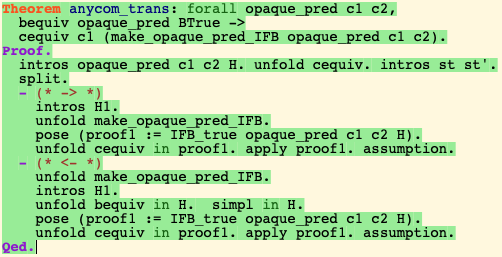
\includegraphics[scale=0.6]{anycom_trans}
        \caption{Coq proof of Theorem \ref{generalcequiv}.}
        \label{fig:generalcequiv}
        \end{figure}

    After the first line of \verb$intros$ and \verb$unfold$s, our goal is to prove command equivalence \eqref{commequiv}, which is the following if-and-only-if statement.
    
\begin{verbatim}
c1 / st \\ st' <->
  make_opaque_pred_IFB opaque_pred c1 c2 / st \\ st'
\end{verbatim}
We \verb$split$ the bi-implication into the two respective one-directional implications.  
\begin{verbatim}
______________________________________(1/2)
c1 / st \\ st' ->
make_opaque_pred_IFB opaque_pred c1 c2 / st \\ st'
______________________________________(2/2)
make_opaque_pred_IFB opaque_pred c1 c2 / st \\ st' ->
c1 / st \\ st'
\end{verbatim}
Focusing on the forwards direction, \verb$intro$ducing the hypothesis and \verb$unfold$ing gives us this proof state.
\begin{verbatim}
opaque_pred : bexp
c1, c2 : com
H : bequiv opaque_pred BTrue
st, st' : state
H1 : c1 / st \\ st'
______________________________________(1/1)
(IFB opaque_pred THEN c1 ELSE c2 FI) / st \\ st'
\end{verbatim}
The next line of the proof contains two new elements.  The first is the theorem \verb$IFB_true$, proven in the Software Foundations library for IMP equivalence, which is the following.
\begin{verbatim}
IFB_true
     : forall (b : bexp) (c1 c2 : com),
       bequiv b BTrue ->
       cequiv (IFB b THEN c1 ELSE c2 FI) c1 
\end{verbatim}
That is, \verb$IFB_true$ states that as long as a boolean expression \verb$b $is boolean equivalent to the constant \verb$BTrue$, then \verb$IFB b THEN c1 ELSE c2 FI$ is command equivalent to \verb$c1$ for any commands \verb$c1$, \verb$c2$.
\par We use \verb$pose$\index{pose} to introduce a new hypothesis with \verb$IFB_true$.  As arguments, we pass our arbitrary opaque predicate and the two states, but also the existing hypothesis \verb$H : bequiv opaque_pred BTrue$, so that our new hypothesis is just the ``then" part of the if-then statement of \verb$IFB_True$.
\begin{verbatim}
proof1 := IFB_true opaque_pred c1 c2 H
 : cequiv (IFB opaque_pred THEN c1 ELSE c2 FI) c1
\end{verbatim}
Next, we \verb$unfold cequiv in proof1$ to turn it into the form below.
\begin{verbatim}
proof1 := IFB_true opaque_pred c1 c2 H
 : forall st st' : state,
   (IFB opaque_pred THEN c1 ELSE c2 FI) / st \\ st' <->
   c1 / st \\ st'
\end{verbatim}
Now \verb$apply$ing \verb$proof1$ to our goal replaces one side of the if-and-only-if with the other, so that our goal changes to
\begin{verbatim}
c1 / st \\ st'
\end{verbatim}
But this is precisely an existing \verb$assumption$, so we are done.
\par The details of the reverse implication are analogous.
\end{proof}
\end{theo}

The power of proving a theorem to this level of generality is that now, the particular programs and predicate used are irrelevant and can be swapped with anything, so long as we can prove the fact that the predicate supplied is indeed an opaque predicate.

\begin{example}\label{factopaqueex}
We can now apply this theorem to our same running example of predicate and factorial program as before.
\begin{verbatim}Example example_fact_opaque_pred: cequiv fact_nonzero 
  (make_opaque_pred_IFB (make_opaque_pred 
     ((X + 1) * (X + 1)) (X * X + X + X + 1)) fact_nonzero SKIP).
\end{verbatim}
\begin{proof}
    The proof is straightforward, after applying Theorem \ref{generalcequiv}, all we need to do is prove the predicate given is indeed equivalent to the constant \verb$BTrue$, and from there it suffices (modulo unfolding some definitions and intros) to apply our previous Lemma \eqref{opaqueness}.
    
\noindent        \begin{figure}[H]
        \centering
        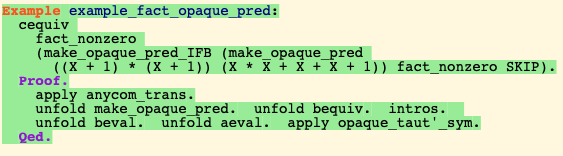
\includegraphics[scale=0.6]{fact_eg}
        \caption{Coq proof of Example \ref{factopaqueex}.}
        \label{fig:factopaqueex}
        \end{figure}
\end{proof}
\end{example}

\section{Hoare logic - weakened information simulation}\label{weakened}

We close this chapter with a series of examples that formally demonstrates the obfuscating effect of using an opaque predicate from the point of view of a simulated attacker.  We use Hoare Logic with the factorial program again, with input $X=3$, output $Y=6$, and with the following concrete dummy program.

\begin{verbatim}
Definition square_program : com := Y ::= X * X.
\end{verbatim}

Next, we'll define an obfuscated program obtained by using the transformations defined in the previous section, with the factorial program as the target of the obfuscation, the same running opaque predicate, and this \verb$square_program$ as the dummy program, which squares the input $X$ and outputs as $Y$.

\begin{verbatim}
Definition trans_fact_square_program : com :=
  (make_opaque_pred_IFB (make_opaque_pred 
    ((X + 1) * (X + 1)) (X * X + X + X + 1)) fact_program square_program).
\end{verbatim}

\begin{example}\label{hoare21}
    With the original factorial program, it is a straightforward application of the more general theorem already proven that the Hoare triple \[(|X=3|)\ fact\_program\ (|Y=6|)\] is valid.
    \begin{proof} 
    \noindent        \begin{figure}[H]
        \centering
        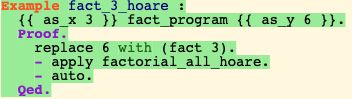
\includegraphics[scale=0.6]{hoare21}
        \caption{Coq proof of Example \ref{hoare21}.}
        \label{fig:hoare21}
        \end{figure}
    
    Here we see the first use of \verb$replace$\index{replace}, which replaces all instances of its first argument with its second argument, but adds the goal to prove that they are actually equal.  In this, \verb$auto$ is able to prove that $6=3!$.
    \end{proof}
\end{example}

\begin{example}\label{hoare22}
With the transformed program, the analogous Hoare triple
\[(|X=3|)\ trans\_fact\_square\_program\ (|Y=6|)\]
is valid.
\begin{proof}
\noindent\begin{figure}[H]
        \centering
        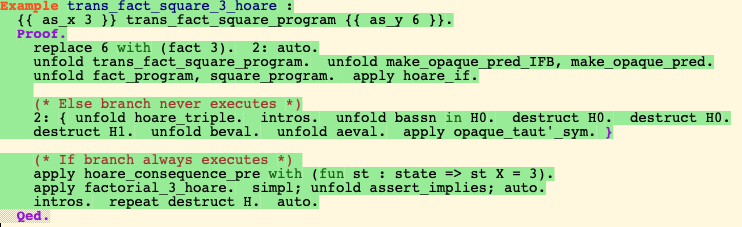
\includegraphics[scale=0.6]{hoare22}
        \caption{Coq proof of Example \ref{hoare22}.}
        \label{fig:hoare22}
        \end{figure}
Note here, however, that by using \verb$apply opaque_taut'_sym$ in the if-else branch to show it can never execute, we are using the known fact that our opaque predicate indeed always evaluates to true!
\end{proof}
\end{example}

\begin{example}\label{hoare23}
Now to simulate an attacker\footnote{This thesis is primarily focused on correctness rather than security models.  We're just assuming that we have an attacker performing static analysis on the code, and that he or she doesn't know the opaque predicate is always true or always false.  Under that assumption, we show that they obtain weaker information than they otherwise would have.} who does not understand the opaque predicate, we show that the best information that can be gleamed is that the output is either $6$ or $9$; the proof must proceed through both the if-then and if-else branch, and the final post-condition weakened to the disjunction of the two possible outcomes, yielding the Hoare triple
\[
(|X=3|)\ trans\_fact\_program\ (|Y=6 \lor Y=9|).
\]
\begin{proof}
\noindent\begin{figure}[H]
        \centering
        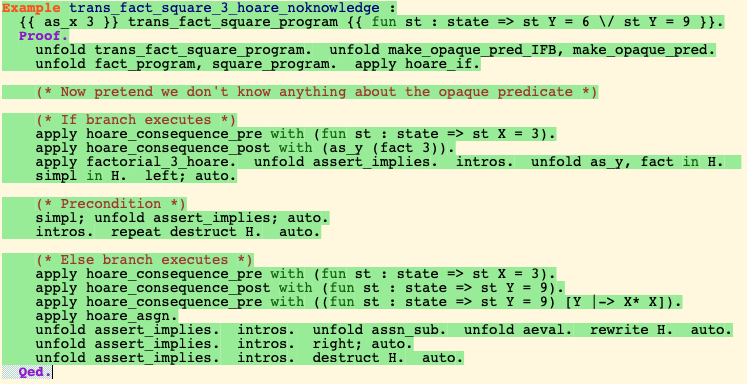
\includegraphics[scale=0.6]{hoare23}
        \caption{Coq proof of Example \ref{hoare23}.}
        \label{fig:hoare23}
        \end{figure}
\end{proof}
\end{example}

\begin{rem}
    We kindly ask the reader to suspend their disbelief that an attacker intelligent enough to understand Hoare logic could not at a glance recognize a kindergarten polynomial identity.  The purpose of the example is simply to give a formal demonstration of how information gained by analyzing a program is weakened in the event that one cannot recognize the opaque predicate as such.
    \par If it makes the reader sleep better at night, the opaque predicate in the final example above can be replaced with something much more difficult\footnote{Just about any number-theoretic tautology will do.  One example of something less obvious given in \cite{CoNa} is $\forall x, y \in \Z, x^2 - 34y^2 \neq 1$.}, and the proof would go exactly the same since, after all, we're pretending we \emph{don't} have a proof that the predicate has a constant truth valuation.
\end{rem}

\chapter{Control flow flattening in IMP/Coq}\label{Ch4}
Reverse engineering tools such as the one we saw in the Introduction can at a glance reveal some information about the \define{control flow} of the program, or the rough structure as delineated by the flow of blocks of code through If-Then-Else, While-Do-End, Switch, and Jump constructs.

\par The obfuscation technique to make this difficult to analyze, then, is \define{control flow flattening}, which aims to break apart all of these constructs that would reveal information about a program's control flow, and flatten an entire program into a single semantically equivalent switch statement inside a while loop.

\par Control flow flattening obfuscation of C++ programs is studied in \cite{Laszlo}, and a treatment of its effects in obstructing static analysis can be found in \cite{Wang}.  

\par This chapter can be divided into two distinct halves.  In the former, we study the flattening of an If-Then-Else construct, adding switch statements directly to the semantics of IMP, then formalizing and proving sound a general transformation algorithm.  In the latter, we study the dismantling and flattening of a While-Do-End structure found in the literature, and define a flowchart language to wrap around IMP, in order to formalize and prove the result of a modified version of an example.

\section{Flattening an If-Then-Else construct}
For the first half of this chapter, we will focus in on a single transformation that turns an If-Then-Else construct
\[
\xymatrix{
& Header \ar[d] & \\
& If\ (b) \ar[dl]_{true} \ar[dr]^{false} & \\
c1\ar[dr] & & c2\ar[dl] \\
& Footer &
}
\]
into the following equivalent flattened program.
\[
\xymatrixrowsep{1cm}
\xymatrixcolsep{0.4cm}
\xymatrix{
 &  s = 0 \ar[d]  & \\
  & While\ (s <= 4)\ do\ (Switch\ s)\ End \ar[dl]_{case\ 0} \ar[ddl]^{case\ 1} \ar[dd]^{case\ 2} \ar[ddr]_{case \ 3} \ar[dr]^{case\ 4}  & \\
Header;\ s = 1 &   & Footer;\ s = 5 \\
If\ (b)\ then\ (s = 2)\ else\ (s = 3)& c1;\ s = 4& c2 ;\ s = 4}
\]

We will, in Section \ref{4.2}, first add the syntax and semantics of Switch statements to the IMP language.  Then in Section \ref{4.3} we formalize the above transformation, define what it means for it to be correct, realize some additional conditions are required and formulate what those are, and then finally prove it so.


\section{Augmenting IMP with Switch (IMP+Switch)}\label{4.2}
Before we can formalize control flow flattening of an If-Then-Else construct, we need to enrich IMP with the syntax and semantics of switch statements, which we'll call the \define{IMP+Switch} language.  To this end, we edit a copy of the IMP file\footnote{The Coq file, part of \cite{Pier}, which defines the IMP language.}, which is named \verb$SF_Imp_Switch.v$ in the repo \cite{repo}.

\par We'll define a new type, \verb$address$, which is just a wrapper for a \verb$nat$ and a type \verb$lc$ (list of commands) which is a list of possible switch branches indexed by \verb$address$, and then redefine the type \verb$com$ to support switch statements.

\begin{verbatim}
Definition address := nat.
\end{verbatim}

\begin{defin}[(IMP) command, augmented with Switch]
We add the constructor \verb$CSwitch$, below, to the original definition given in \eqref{impcommand}.
\begin{verbatim}
Inductive com : Type :=
  | CSkip : com
  | CAss : string -> aexp -> com
  | CSeq : com -> com -> com
  | CIf : bexp -> com -> com -> com
  | CWhile : bexp -> com -> com
  | CSwitch : string -> list (address * com) -> com. (** <-- New! **)
\end{verbatim}

The notation we define for switch statements is as follows.

\begin{verbatim}
Notation "'SWITCH' var swDict" := (CSwitch var swDict) 
  (at level 80, swDict at level 1, var at level 5, right associativity) 
    : com_scope.
\end{verbatim}
\end{defin}

To make the lists of addresses and commands easier to work with, we'll define a wrapper type \verb$lc$.

\begin{verbatim}
Definition lc := list (address * com).
\end{verbatim}

We now take a brief digression to introduce the \define{option} type, whose purpose is to represent partial functions.
\interfootnotelinepenalty=10000
\newpage
\begin{defin}[Option type]
For any type $A$, the type $option\ A$ consists of $None$ and $Some\ a$ for any term $a$ of $A$\footnote{For example, suppose the type $A$ is the natural numbers $\N$.  The type $Option\ \N$ consists of precisely the following terms (or elements, in set-theoretic language): $None$, $Some\ 0$, $Some\ 1$, $Some\ 2$, $Some\ 3$, $\ldots$
\par The idea is that this enables us to express a function that may not be defined at certain inputs.  For example, suppose we wish to define a partial function from $\N$ to $\N$ which maps every number from 1 to 100 to itself but is undefined on any larger number.  Set-theoretically, this function's graph the set of ordered pairs
$\{(n,n)\ |\ n\leq 100\}$ as a partial identity function from $\N$ to $\N$,
implicitly considered undefined for $n > 100$.
\par In Coq, we explicitly define a function $f\colon \N \to Option \ \N$, where $f(n) = Some\ n$ if $n \leq 100$ and $f(n) = None$ otherwise.  Set-theoretically, this would be
like defining the partial function $f$ by the graph 
$\{(n,\ Some\ n)\ |\  n\leq 100\} \cup \{(n,\ None)\ |\ n > 100\}$.
}.  In Coq,
\begin{verbatim}
Inductive option (A : Type) : Type :=
    | Some : A -> option A 
    | None : option A.
\end{verbatim}
The idea is that if we wish to represent a partial function $f\colon A \to B$, we instead declare in Coq a total function $f_o\colon A \to option\ B$ with $f_o(a) = Some\ b$ if $f(a)$ is defined and $f(a)=b$, and $f_o(a) = None$ if $f(a)$ is undefined.
\end{defin}

Next, we create a function to search a \verb$lc$.

\begin{defin}[Command list lookup function]
The following is a recursive helper function that searches a \verb$lc$ by address.
\begin{verbatim}Fixpoint lc_lookup (tlc : lc) (adr : address) : option com :=
  match tlc with
  | [] => None
  | (adr', c')::tail => if (beq_nat adr adr') 
                           then Some c'
                           else lc_lookup tail adr
  end.\end{verbatim}
  If the list argument \verb$tlc$ is nonempty, then we are in the second case, where \verb$(adr', c')$ is the head (first element) of the list, and \verb$tail$ is the tail (list consisting of the remaining elements of the list).  
  \par Now, if the address \verb$adr'$ of the head element is equal to the address argument \verb$adr$, then we have a match, and the command portion \verb$c'$ of the head element is returned as the option command \verb$Some c'$.  If the addresses do not match up, then we recursively call the lookup on the tail of the list with the same address to search for.
  \par Each recursive call shrinks the length of the list being searched through by 1, until we either find the address we're looking for, or we've gone through the entire original list, in which case the final recursive call is on an empty list, which is in the first case and returns \verb$None$.
\end{defin}

We can now redefine the command evaluation semantics to include switch statements.

\begin{defin}[Command evaluation (with switch)]\index{command evaluation!with switch}
\begin{verbatim}

Inductive ceval : com -> state -> state -> Prop :=
  | E_Skip : forall st,
      SKIP / st \\ st
  | E_Ass  : forall st a1 n x,
      aeval st a1 = n ->
      (x ::= a1) / st \\ (st & { x --> n })
  | E_Seq : forall c1 c2 st st' st'',
      c1 / st \\ st' ->
      c2 / st' \\ st'' ->
      (c1 ;; c2) / st \\ st''
  | E_IfTrue : forall st st' b c1 c2,
      beval st b = true ->
      c1 / st \\ st' ->
      (IFB b THEN c1 ELSE c2 FI) / st \\ st'
  | E_IfFalse : forall st st' b c1 c2,
      beval st b = false ->
      c2 / st \\ st' ->
      (IFB b THEN c1 ELSE c2 FI) / st \\ st'
  | E_WhileFalse : forall b st c,
      beval st b = false ->
      (WHILE b DO c END) / st \\ st
  | E_WhileTrue : forall st st' st'' b c,
      beval st b = true ->
      c / st \\ st' ->
      (WHILE b DO c END) / st' \\ st'' ->
      (WHILE b DO c END) / st \\ st''

  (* New: Switch. *)
  | E_Switch: forall var n swDict c st st',
      aeval st (AId var) = n ->                       
      lc_lookup swDict n = Some c ->                  
      c / st \\ st' ->                           
      (SWITCH var swDict) / st \\ st' 
               
where "c1 '/' st1 '\\' st2" := (ceval c1 st1 st2).
\end{verbatim}
For the command \verb$SWITCH var swDict$ to take a state \verb$st$ to a state \verb$st'$ means that, in state \verb$st$, the variable \verb$var$ evaluates to some natural number \verb$n$, that looking up the list \verb$swDict$ with \verb$n$ yields \verb$Some c$, and that \verb$c $takes the state \verb$st$ to \verb$st'$.
\end{defin}

The following theorem will be necessary in the main result of the first half of this chapter.  This theorem and its proof already exist in \cite{Pier}, but we must update it for our new formulation with switch statements.  The proof also introduces several new tactics and features which are worth explaining.

\begin{theo}\label{deterministic}\index{deterministic}
Command evaluation is deterministic, in the sense that if a command evaluates a state $st$ to a state $st1$, but also to some (a priori, possibly) other state $st2$, then it must be the case that $st1 = st2$.  In Coq,
\begin{verbatim}
Theorem ceval_deterministic: forall c st st1 st2,
  c / st \\ st1 -> c / st \\ st2 -> st1 = st2.
\end{verbatim}
\begin{proof}
\noindent
\begin{figure}[H]
        \centering
        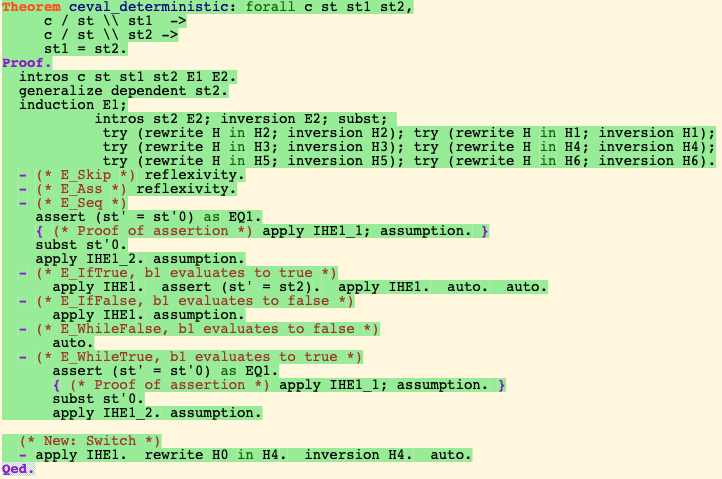
\includegraphics[scale=0.6]{ceval_deterministic}
        \caption{Coq proof of Theorem \ref{deterministic}.}
        \label{fig:deterministic}
        \end{figure}
After the first line of \verb$intros$, we have the following proof state.
\begin{verbatim}
c : com
st, st1, st2 : state
E1 : c / st \\ st1
E2 : c / st \\ st2
______________________________________(1/1)
st1 = st2
\end{verbatim}
However, in order for this proof to go through, it is necessary that \verb$st2$ be left as an arbitrary state for the moment, rather than instantiated.  Since \verb$intros$ goes in order of appearance of universally quantified variables, there was no way to not instantiate \verb$st2$ but instantiate \verb$E1$.  
\par Thus, we use the tactic \verb$generalize dependent$\index{generalize} on \verb$st2$ to tell Coq that we want to leave it as universally quantified, resulting in this proof state, which also removes \verb$E2$ which was dependent on \verb$st2$
\begin{verbatim}
c : com
st, st1 : state
E1 : c / st \\ st1
______________________________________(1/1)
forall st2 : state, 
  c / st \\ st2 -> st1 = st2
\end{verbatim}
Next, we meet the semicolon, which will apply subsequent tactics (on the right) on every subgoal generated by the tactic on the left.  In this case, \verb$induction E1$ generates 8 subgoals, corresponding to the possible ways this command evaluation was constructed (depending on the forms the command \verb$c $takes).  Then, \verb$intros st2 E2$ is applied to each of those 8 subgoals, and so on so forth.  
\par After \verb$induction E1; intros st2 E2; inversion E2; subst$, we have 12 subgoals.  We'll slow down for a moment and explain the new tactics on the first generated subgoal.  The tactic \verb$inversion$\index{inversion} analyzes a hypothesis and discovers conditions that are necessary for it to be true, and gives us those as well.  For example, in the first case, we have
\begin{verbatim}
E2 : SKIP / st \\ st2
\end{verbatim}
whence \verb$inversion E2$ yields the new hypotheses
\begin{verbatim}
st0 : state
H0 : st0 = st
H1 : st = st2
\end{verbatim}
evident from the fact that \verb$SKIP$ can only take one state to another if they are in fact the same state.  As we will see later, \verb$inversion$ is also able to recognize when a hypothesis is impossible in the current proof state, completing a proof by contradiction. 
\par Applying \verb$subst$\index{subst} (substitution) then automatically rewrites and then erases any equalities in all existing hypotheses and goal(s), removing the three generated by \verb$inversion$ above and changing rewriting the original to
\begin{verbatim}
E2 : SKIP / st2 \\ st2.
\end{verbatim}
\par Now, four of these 12 subgoals correspond to impossible cases, i.e.\ that the constructor \verb$E_IfTrue$ was invoked but the boolean \verb$b1$ was false, or \verb$E_IfFalse$ was invoked with \verb$b1$ true, and similarly for \verb$E_WhileTrue$ and \verb$E_WhileFalse$ respectively.  
\par After going through dispatching these cases, we noticed some common patterns in these cases, and to keep the proof clean we deal with all of these immediately.  The tactical \verb$try$\index{try} will, as the name suggests, try the tactic it is passed on the goal (recall that these appear after semicolons, so these are applied also on the 8 nondegenerate cases), but will not cause an error if the tactic does not succeed.
\par As seen in the comments in the screenshot, the proof now proceeds to the 8 possible cases and we prove the statement in each case.  We'll omit the explanation of the first seven, which appear in \cite{Pier} and don't contain any new tactics we haven't met yet.
\par For the final case, the induction is on the evaluation of a switch statement, and we have the following proof state after focussing.
\begin{verbatim}
var : string
swDict : lc
c : com
st, st' : state
H0 : lc_lookup swDict (aeval st var) = Some c
E1 : c / st \\ st'
IHE1 : forall st2 : state, c / st \\ st2 -> st' = st2
st2 : state
E2 : (SWITCH var swDict) / st \\ st2
c0 : com
H4 : lc_lookup swDict (aeval st var) = Some c0
H7 : c0 / st \\ st2
______________________________________(1/1)
st' = st2
\end{verbatim}
Note here the inductive hypothesis \verb$IHE1$ quantifies over all states \verb$st2$, instead of a particular one.  Requiring this level of generality is the reason why we had to use \verb$generalize dependent st2$ at the start of the proof.  After we \verb$apply IHE1$, the goal changes to
\begin{verbatim}
c / st \\ st2.
\end{verbatim}
Next, \verb$rewrite H0 in H4$ changes that hypothesis to
\begin{verbatim}
H4 : Some c = Some c0
\end{verbatim}
which we then use \verb$inversion$ on, yielding the fact that it must have been the case that
\begin{verbatim}
H1 : c = c0
\end{verbatim}
which means the goal is equivalent to
\begin{verbatim}
c0 / st \\ st2
\end{verbatim}
which is precisely \verb$H7$, and so can be finished with \verb$auto$.
\end{proof}
\end{theo}

\section{Flattening If-Then-Else in IMP+Switch}\label{flattenif}\label{4.3}
We now aim to formalize the transformation described at the start of the chapter, and prove it correct.  This code can be found in the file $OBFS\_flatten.v$ in  \cite{repo}.  First, we will give a name to the switching variable introduced.

\begin{verbatim}
Definition swVar : string := "swVar".
\end{verbatim}

Now, we wish to prove command equivalence between the original and transformed programs, so we note that \verb$swVar$ is introduced with value $0$ and ends with value $5$ in the transformed program; hence, we'll preprocess the original program to be transformed by adding in these assignments.

\begin{defin}
Preprocessing a program with an If-Then-Else statement to be flattened is the following function in Coq.
\begin{verbatim}
Definition preprocess_program header cond c1 c2 footer : com :=
  swVar ::= 0 ;;
  header ;;
  IFB cond THEN 
    c1 
  ELSE 
    c2 
  FI ;;
  footer ;;
  swVar ::= 5.
\end{verbatim}
\end{defin}

\begin{defin}
Transforming a program with control flow flattening on an If-Then-Else statement is the following function in Coq.
\begin{verbatim}
Definition transform_program header cond c1 c2 footer : com :=
  swVar ::= 0 ;;
  WHILE (swVar <= 4) DO
    SWITCH swVar [
      (0, header ;; 
          swVar ::= 1) ;
      (1, IFB cond THEN
            swVar ::= 2 
          ELSE 
            swVar ::= 3 
          FI) ;
      (2, c1 ;;
          swVar ::= 4) ;
      (3, c2 ;;
          swVar ::= 4) ;
      (4, footer ;;
          swVar ::= 5)
    ]
  END.
\end{verbatim}
\end{defin}

\begin{defin}[WorldEater program]
We'll use a minimal example program for this section, which we call \define{WorldEater}, a program that does nothing if the variable $X$ is zero, and assigns $X=1$ otherwise.

\begin{verbatim}
Definition WorldEater : com :=
  IFB (X = 0) THEN
    SKIP
  ELSE
    X ::= 1
  FI.
\end{verbatim}
\end{defin}

\begin{example}
To preprocess $WorldEater$, we feed its components to \verb$preprocess_program$.
\begin{verbatim}
Definition PreprocessWorldEater := 
  preprocess_program SKIP (X = 0) SKIP (X ::= 1) SKIP.
\end{verbatim}
We can then ask Coq to display the result with \verb$compute PreProcessWorldEater$.
\begin{verbatim}
"swVar" ::= 0;;
SKIP;;
(IFB "X"%string = 0 THEN SKIP ELSE "X" ::= 1 FI);;
SKIP;; 
"swVar" ::= 5
\end{verbatim}
Note that since the header and footer are mandatory, we add \verb$SKIP$s, and the \verb$swVar$ is set to the same initial and final values so we can prove command equivalence to the transformed program.
\end{example}

\begin{example}
To transform $WorldEater$, we feed its components to \verb$transform_program$.
\begin{verbatim}
Definition TransWorldEater := 
  transform_program SKIP (X = 0) SKIP (X ::= 1) SKIP.
\end{verbatim}
Again, we display the result, with \verb$compute TransWorldEater$.
\begin{verbatim}
"swVar" ::= 0;;
WHILE "swVar"%string <= 4 DO SWITCH "swVar"
    [(0, SKIP;; "swVar" ::= 1);
     (1, IFB "X"%string = 0 THEN "swVar" ::= 2
         ELSE "swVar" ::= 3 FI); 
     (2, SKIP;; "swVar" ::= 4);
     (3, "X" ::= 1;; "swVar" ::= 4);
     (4, SKIP;; "swVar" ::= 5)] END
\end{verbatim}
\end{example}

\noindent We now need a lemma about updating maps to prove the upcoming main result.  It is relatively straightforward; the only new tactic we see is the application of \verb$functional_extensionality$\index{functional extensionality}, which says that two functions are equal precisely when their action agrees on all possible elements (or terms, since we are working in type theory).  So in Coq, when we have a goal of $f=g$ for two functions $f,g: A \to B$, applying functional extensionaltiy changes the goal to $\forall a \in A, f(a) = g(a)$.

\begin{lem}\label{update_shadow}
Updating a map by assigning a variable $X$ twice is the same as only updating it with the second assignment.  In Coq,
\begin{verbatim}
Lemma t_update_shadow : forall A (m: total_map A) v1 v2 x,
    m & {x --> v1 ; x --> v2} = m & {x --> v2}.
\end{verbatim}
\begin{proof}\noindent
   \begin{figure}[H]
        \centering
        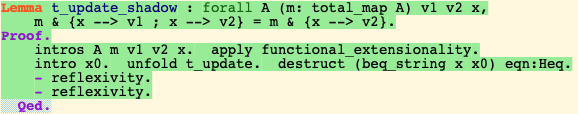
\includegraphics[scale=0.6]{lemma_final_1}
        \caption{Coq proof of Lemma \ref{update_shadow}.}
        \label{fig:hoare21}
        \end{figure}
\end{proof}
\end{lem}

\begin{comment}
\begin{lem}\label{update_commutative}
Updating a map with the assignment of $X = v_1$ and then $Y = v_2$ is the same as first updating with $Y = v_2$ and then $X = v_1$, as long as $X \neq Y$.
\begin{proof}\ \newline
    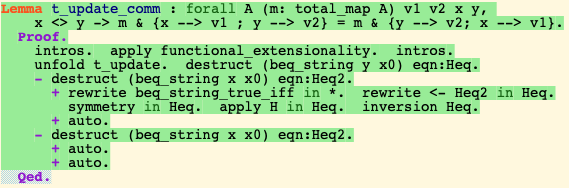
\includegraphics[scale=0.6]{lemma_final_2}
\end{proof}
\end{lem}
\end{comment}

\begin{example}\label{WE_example}
The preprocessed and transformed $WorldEater$ program are command equivalent.  In Coq,
\begin{verbatim}
Example WorldEaterTransEquiv : 
  cequiv PreprocessWorldEater TransWorldEater.
\end{verbatim}
The proof follows the same structure and ideas as the more general Theorem \ref{maintheo} to come.
\end{example}

We now wish to generalize this example, and state a general theorem that all programs' preprocessed and transformed forms are command equivalent.  We actually attempted to do it directly as-is, and ran into problems during the proof, which prompted inquiry into what the problem was, and how to resolve it.  In fact, it is the exact same problem we left open at the end of Non-theorem \ref{hoarefail}, which we now explain and offer the solution for.

\par The problem with simply stating that for all programs in the Header-If-Then-Else-Footer structure we have, their preprocessed and transformed versions are command equivalent, is the fact that we haven't fully accounted for the newly introduced \verb$swVar$ which controls the switch statement.  If the original program already uses this variable in some way, then everything could break.  For example, suppose the header of a program to be transformed contains the assignment \verb$swVar := 999$.  This would then completely bypass the entire flattened switch construct!

\par The next idea, then, is to state that as long as the program being transformed doesn't make use of \verb$swVar$ in any way, then we get the desired result.  Although this is intuitively true, this is exceedingly difficult to express in our formal language of Coq proofs.  Thus, we come up with some invariance conditions that are easier to express and strong enough to imply the desired outcome.

\begin{defin}[Evaluation invariance]\index{evaluation invariance}
A program $c$ is \emph{evaluation invariant} with respect to a variable $X$ if, for all states $st$ and $st'$ and all $n \in \N$, $c$ evaluates $st$ to $st'$ if and only if $c$ evaluates $st$ updated with $(X \longrightarrow n)$ to $st'$ updated with $(X\longrightarrow n)$.
\par In other words, if the only thing that changes about the start state is the value of $X$, there is no impact on evaluation with the sole exception of the same change to $X$ in the end state.  In Coq,
\begin{verbatim}
Definition eval_invariant c X := forall n st st', 
    c / st \\ st' <-> c / st & { X --> n } \\ st' & { X --> n }.
\end{verbatim}
\end{defin}

\begin{defin}[Boolean invariance]\index{boolean invariance}
A boolean expression $b$ is \emph{boolean invariant} with respect to a variable $X$ if for all states $st$ and all $n \in \N$, the boolean evaluation of $b$ in $st$ is the same as the boolean evaluation of $b$ in $st$ updated with $(X\longrightarrow n)$.
\par In other words, if the only thing that changes about the state in which boolean evaluation takes place is the value of $X$, then there is no impact on the evaluation.  In Coq,
\begin{verbatim}
Definition beval_invariant b X :=
  forall n st, beval st b = beval (st & { X --> n }) b. 
\end{verbatim}
\end{defin}

\begin{lem}\label{independence}
Evaluation invariance implies evaluation independence in the sense that, if a command $c$ is evaluation invariant with respect to $X$, then if $c$ evaluates a state $st$ updated with $(X\longrightarrow n)$ for some $n \in \N$ to $st'$, then $c$ also evaluates $st$ to $st'$.  In Coq,
\begin{verbatim}
Lemma eval_inv_imp_eval_ind : forall c X n st st', 
  eval_invariant c X ->
  c / st & { X --> n } \\ st' -> 
  c / st \\ st'.
\end{verbatim}
\begin{proof}\noindent
    \begin{figure}[H]
        \centering
        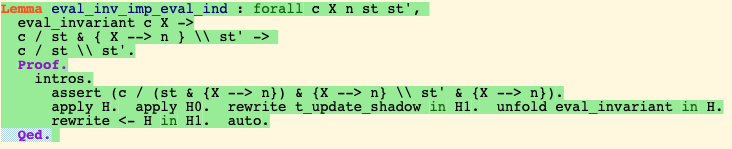
\includegraphics[scale=0.6]{lemma_final_3}
        \caption{Coq proof of Lemma \ref{independence}.}
        \label{fig:independence}
        \end{figure}
\end{proof}
\end{lem}

\begin{theo}\label{maintheo}
Control flow flattening of If-Then-Else constructs is sound in the following sense.  
\par Fix the variable \verb$swVar$ for the control flow flattening transformation.  For any program of the form \verb$header ;; IFB cond THEN c1 ELSE c2 END ;; footer$, we have command equivalence between the programs
\begin{verbatim}preprocess_program header cond c1 c2 footer\end{verbatim}
and
\begin{verbatim}transform_program header cond c1 c2 footer\end{verbatim}
as long as the following hold:
\begin{itemize}
    \item The commands \verb$footer$, \verb$c1$, and \verb$c2$ are evaluation invariant with respect to \verb$swVar$.
    \item The boolean condition \verb$cond$ is boolean invariant with respect to \verb$swVar$.
\end{itemize}
In Coq,
\begin{verbatim}
Theorem AllTransEquiv : forall header cond c1 c2 footer, 
  eval_invariant c1 swVar -> eval_invariant c2 swVar -> 
  eval_invariant footer swVar -> beval_invariant cond swVar ->
  cequiv (preprocess_program header cond c1 c2 footer) 
    (transform_program header cond c1 c2 footer).
\end{verbatim}
\begin{proof}
    The proof of this theorem is long, so we will break down the screenshots and explanations into discrete sub-parts.  We will explain one of two cases, and one of four subcases in detail.
    
    \par The statement of the theorem and initial setup of the proof is below.
    
    \noindent\begin{figure}[H]
        \centering
        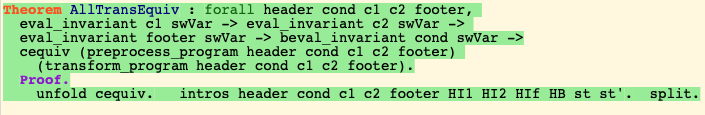
\includegraphics[scale=0.6]{alltrans_main}
        \caption{Coq formulation of Theorem \ref{maintheo}.}
        \label{fig:maintheo}
        \end{figure}
    
    \noindent After \verb$unfold$ing, \verb$intro$ing, and \verb$split$ting the if-and-only-if of \verb$cequiv$'s definition, our proof state is as follows.
    
    \begin{verbatim}
2 subgoals
header : com
cond : bexp
c1, c2, footer : com
HI1 : eval_invariant c1 swVar
HI2 : eval_invariant c2 swVar
HIf : eval_invariant footer swVar
HB : beval_invariant cond swVar
st, st' : state
______________________________________(1/2)
preprocess_program header cond c1 c2 footer / st \\ st' ->
transform_program header cond c1 c2 footer / st \\ st'
______________________________________(2/2)
transform_program header cond c1 c2 footer / st \\ st' ->
preprocess_program header cond c1 c2 footer / st \\ st'
    \end{verbatim}
    \noindent Case (I) below will correspond to the first goal above, and Case (II) the second.
    \begin{itemize}
        \item[(I)] Preprocessed implies transformed.\ \newline
        \noindent    \noindent\begin{figure}[H]
        \centering
        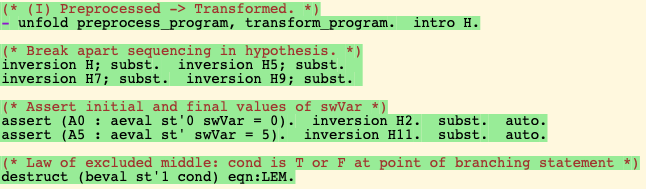
\includegraphics[scale=0.6]{alltrans_1}
        \caption{Coq proof of Theorem \ref{maintheo}, Case (I).}
        \label{fig:maintheo1}
        \end{figure}
        
        After the first line, we've added the hypothesis that the preprocessed program takes \verb$st$ to \verb$st'$, and the goal that the transformed program does the same..
        \begin{verbatim}
H : (swVar ::= 0;; header;; (IFB cond THEN c1 ELSE c2 FI);; 
    footer;; swVar ::= 5) / st \\ st'
______________________________________(1/1)
(swVar ::= 0;; WHILE swVar <= 4 DO SWITCH swVar
    [(0, header;; swVar ::= 1);
    (1, IFB cond THEN swVar ::= 2 ELSE swVar ::= 3 FI);
    (2, c1;; swVar ::= 4); (3, c2;; swVar ::= 4);
    (4, footer;; swVar ::= 5)] END) / st \\ st'\end{verbatim}
        \noindent The hypothesis \verb$H $is about the effect of the entire program on the state, but we wish to break this down, hence the sequence of \verb$inversion$s followed by \verb$subst$s for cleanup.   This has turned \verb$H $into multiple hypotheses, along with newly instantiated intermediate states.
        \begin{verbatim}
st'0 : state
H2 : (swVar ::= 0) / st \\ st'0
H5 : (header;;
      (IFB cond THEN c1 ELSE c2 FI);; footer;; swVar ::= 5) /
     st'0 \\ st'
st'1 : state
H3 : header / st'0 \\ st'1
H7 : ((IFB cond THEN c1 ELSE c2 FI);; footer;; swVar ::= 5) /
     st'1 \\ st'
st'2 : state
H4 : (IFB cond THEN c1 ELSE c2 FI) / st'1 \\ st'2
H9 : (footer;; swVar ::= 5) / st'2 \\ st'
st'3 : state
H6 : footer / st'2 \\ st'3
H11 : (swVar ::= 5) / st'3 \\ st'\end{verbatim}
\noindent Next, a pair of \verb$assert$ions give us new hypotheses of the value of \verb$swVar$ at the first and final states.  These are proven by \verb$invert$ing the correct hypotheses above, and then rewriting with \verb$subst$.
\begin{verbatim}
A0 : aeval st'0 swVar = 0
A5 : aeval st' swVar = 5
\end{verbatim}
\noindent Next, we condition on whether the boolean condition of the If statement is true or false, with \verb$destruct (beval st'1 cond) eqn:LEM$.  The latter part tells Coq that we want to keep this hypothesis around in the proof state with the supplied name.  This generates two subgoals within this branch, corresponding to the cases where \verb$cond$ is true and where it is false, respectively.  We label these as Case (I.i) and Case (I.ii).
            \begin{itemize}
                \item[(I.i)] Preprocessed implies transformed; boolean condition is true.
                
                \noindent\begin{figure}[H]
        \centering
        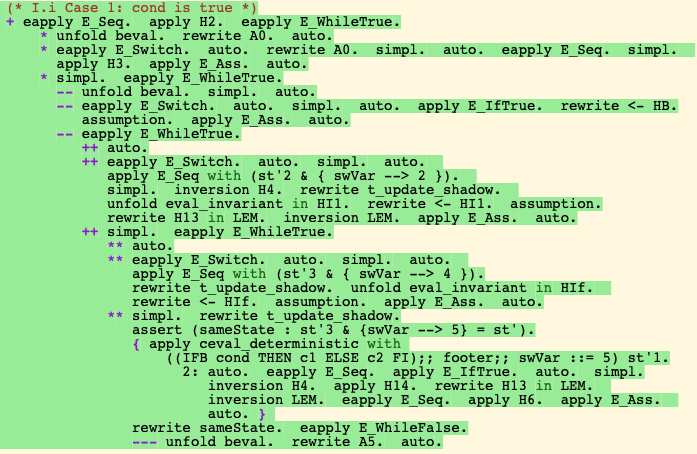
\includegraphics[scale=0.6]{alltrans_1_1}
        \caption{Coq proof of Theorem \ref{maintheo}, Case (I.i).}
        \label{fig:maintheo1}
        \end{figure}
                
                \noindent We have the new hypothesis
                \begin{verbatim}
LEM : beval st'1 cond = true.\end{verbatim}
                \noindent We \verb$eapply E_Seq$ to break the initial assignment off from the main while loop of the transformed program in the goal.
\begin{verbatim}
______________________________________(1/2)
(swVar ::= 0) / st \\ ?st'
______________________________________(2/2)
(WHILE swVar <= 4
 DO SWITCH swVar
    [(0, header;; swVar ::= 1);
    (1, IFB cond THEN swVar ::= 2 ELSE swVar ::= 3 FI);
    (2, c1;; swVar ::= 4); (3, c2;; swVar ::= 4);
    (4, footer;; swVar ::= 5)] END) / 
?st' \\ st'\end{verbatim}
                Coq doesn't know immediately what the intermediate state \verb$?st'$ should be, but we already have the hypothesis \verb$H2 : (swVar ::= 0) / st \\ st'0$, thus applying it solves goal 1 and substitutes \verb$st'0$ for the unknown state in goal 2.
                \par Next, we'll use \verb$eapply E_WhileTrue$ for the remaining goal, as we enter the while loop for the first time.  This replaces the goal with the following three.
                \begin{verbatim}
______________________________________(1/3)
beval st'0 (swVar <= 4) = true
______________________________________(2/3)
(SWITCH swVar
 [(0, header;; swVar ::= 1);
 (1, IFB cond THEN swVar ::= 2 ELSE swVar ::= 3 FI);
 (2, c1;; swVar ::= 4); (3, c2;; swVar ::= 4);
 (4, footer;; swVar ::= 5)]) / st'0 \\ 
?st'
______________________________________(3/3)
(WHILE swVar <= 4
 DO SWITCH swVar
    [(0, header;; swVar ::= 1);
    (1, IFB cond THEN swVar ::= 2 ELSE swVar ::= 3 FI);
    (2, c1;; swVar ::= 4); (3, c2;; swVar ::= 4);
    (4, footer;; swVar ::= 5)] END) / 
?st' \\ st'\end{verbatim}
We proved in the parent branch that the initial value in \verb$st'0$ of \verb$swVar$ is 0 and saved this as hypothesis \verb$A0$ (having done it back there also gives it to us in Case (I.ii) below), so the first goal is easily dispatched with a \verb$rewrite$.
\par For the second goal, we \verb$eapply E_Switch$, which generates the goals
\begin{verbatim}
______________________________________(1/3)
aeval st'0 swVar = ?n
______________________________________(2/3)
lc_lookup
  [(0, header;; swVar ::= 1);
  (1, IFB cond THEN swVar ::= 2 ELSE swVar ::= 3 FI);
  (2, c1;; swVar ::= 4); (3, c2;; swVar ::= 4);
  (4, footer;; swVar ::= 5)] ?n = Some ?c
______________________________________(3/3)
?c / st'0 \\ ?st'\end{verbatim}
The first is solved with \verb$auto$, since we already know its value is 0; we also use \verb$rewrite A0$ to turn \verb$?n$ in the second goal into 0, whence a \verb$simpl$e computation reveals that
\begin{verbatim}
Some (header;; swVar ::= 1) = Some ?c
\end{verbatim}
but of course this means the command part of the option commands are also true, so \verb$auto$ leaves us with the remaining goal of
\begin{verbatim}
(header;; swVar ::= 1) / st'0 \\ ?st'
\end{verbatim}
which can be solved with the familiar applications of \verb$E_Seq$, \verb$E_Ass$, and some other straightforward tactics.
\par We've now gone through the first iteration of the while loop, having executed the \verb$header$ part of the program.  This general pattern repeats, with each subsequent level of nesting in the proof being the next iteration of the while loop.  We'll go through the general structure and explain the application of lemmas, sparing the reader from the tedium of a complete play-by-play.
\par The next several lines, kicked off by the line \begin{verbatim}* simpl.  eapply E_WhileTrue\end{verbatim} goes through the second iteration, which goes through the 
\begin{verbatim}
(1, IFB cond THEN swVar ::= 2 ELSE swVar ::= 3 FI);\end{verbatim}
branch of the switch statement, and sets \verb$swVar$ to $2$, as \verb$cond$ is true in this subcase.  Nothing interesting happens in this proof of this part.
\par Continuing then on the next iteration of the while loop, at the line
\begin{verbatim}
-- eapply E_WhileTrue
\end{verbatim}
and after the line \verb$++ auto$ to dispatch the goal of handling the boolean evaluation, we are at the line
\begin{verbatim}
++ eapply E_Switch.  auto.  simpl.  auto.
\end{verbatim}
Here, our goal is
\begin{verbatim}
(c1;; swVar ::= 4) /
st'1 & {swVar --> 1; swVar -->
aeval (st'1 & {swVar --> 1}) 2} \\ ?st'.
\end{verbatim}
We \verb$apply E_Seq with (st'2 & { swVar --> 2 }$, supplying the intermediate state and \verb$simpl$ify, to change the goals to
\begin{verbatim}
______________________________________(1/2)
c1 / st'1 & {swVar --> 1; swVar --> 2} \\
st'2 & {swVar --> 2}
______________________________________(2/2)
(swVar ::= 4) / st'2 & {swVar --> 2} \\ ?st'
\end{verbatim}
We use \verb$inversion$ on \verb$H4 : (IFB cond THEN c1 ELSE c2 FI) / st'1 \\ st'2$, yielding, among others, the new hypothesis
\begin{verbatim}H14: c1 / st'1 \\ st'2\end{verbatim} for the case that \verb$cond$ is true, and also generating another subgoal for the case that \verb$cond$ is false.
\par In the subgoal with \verb$cond$ is true (which we continue inline instead of further focussing, as the proof in the code is already getting quite messy and indented), we use \verb$rewrite t_update_shadow$ (Lemma \ref{update_shadow}) to change the current subgoal to
\begin{verbatim}
______________________________________(1/3)
c1 / st'1 & {swVar --> 2} \\ st'2 & {swVar --> 2}
\end{verbatim}
Next, we \verb$unfold eval_invariant in HI1$, expanding the definition in one of our initial assumptions to
\begin{verbatim}
HI1 : forall (n : nat) (st st' : state),
      c1 / st \\ st' <->
      c1 / st & {swVar --> n} \\ st' & {swVar --> n}.
\end{verbatim}
Now we use the assumed evaluation invariance to \verb${rewrite <-}$ the goal to
\begin{verbatim}
______________________________________(1/3)
c1 / st'1 \\ st'2
\end{verbatim}
which is precisily \verb$H14$, introduced a few lines prior, and so dispatched with \verb$assumption$.
\par In the second subgoal generated by \verb$inversion H4$, we have the hypothesis that
\verb$H13 : beval st'1 cond = false$, but recall that in this entire part of the proof we've assumed it's true; hence, \verb$rewrite H13 in LEM$ yields
\begin{verbatim}LEM : false = true.\end{verbatim}
\par This is some obvious nonsense, so \verb$inversion LEM$ clears this subgoal.  Finally, the remaining assignment subgoal
\begin{verbatim}
______________________________________(1/1)
(swVar ::= 4) / st'2 & {swVar --> 2} \\ ?st'
\end{verbatim}
is solved with \verb$apply E_Ass.  auto.$
\par The next iteration of the while loop goes through the \verb$footer$.  This part begins at the line
\begin{verbatim}++ simpl.  eapply E_WhileTrue.\end{verbatim}
Again there is nothing new here, so we'll skip ahead to the next iteration, where the guard condition of the while loop is no longer true.  Picking up after the line
\begin{verbatim}
** simpl.  rewrite t_update_shadow,
\end{verbatim}
we have the goal 
\begin{verbatim}
______________________________________(1/1)
(WHILE swVar <= 4
 DO SWITCH swVar
    [(0, header;; swVar ::= 1);
    (1, IFB cond THEN swVar ::= 2 ELSE swVar ::= 3 FI);
    (2, c1;; swVar ::= 4); (3, c2;; swVar ::= 4);
    (4, footer;; swVar ::= 5)] END) /
st'3 & {swVar --> 5} \\ st'.
\end{verbatim}
However, the initial and final state in this goal are actually the same, which we declare with
\begin{verbatim}assert (sameState : st'3 & {swVar --> 5} = st').\end{verbatim}
We need to prove the assertion before we can use it, which we do by invoking Theorem \ref{deterministic}, with
\begin{verbatim}
apply ceval_deterministic with 
  ((IFB cond THEN c1 ELSE c2 FI);; footer;; swVar ::= 5) st'1.
\end{verbatim}
That is, we now take the next few lines to prove the following two goals.
\begin{verbatim}
______________________________________(1/2)
((IFB cond THEN c1 ELSE c2 FI);; footer;; swVar ::= 5) /
st'1 \\ st'3 & {swVar --> 5}
______________________________________(2/2)
((IFB cond THEN c1 ELSE c2 FI);; footer;; swVar ::= 5) /
st'1 \\ st'
\end{verbatim}
This is fairly straightforward, and we now get the new hypothesis
\begin{verbatim}
sameState : st'3 & {swVar --> 5} = st'
\end{verbatim}
We \verb$rewrite sameState$ so that our goal now has \verb$st'$ as both the start and end state, and is now in the correct form for \verb$eapply E_WhileFalse$.  All that remains to be done now is to show
\begin{verbatim}
______________________________________(1/1)
beval st' (swVar <= 4) = false.
\end{verbatim}
But after an \verb$unfold$, we \verb$rewrite A5$ (recall this is the assertion we made, what seems now like a lifetime ago, that the value of \verb$swVar$ in the final state is 5).  Coq is smart enough to know \verb$5 <= 4 = false$, and so we finish this subcase with an \verb$auto$.
                \item[(I.ii)] Preprocessed implies transformed; boolean condition is false.
                
                \noindent\begin{figure}[H]
        \centering
        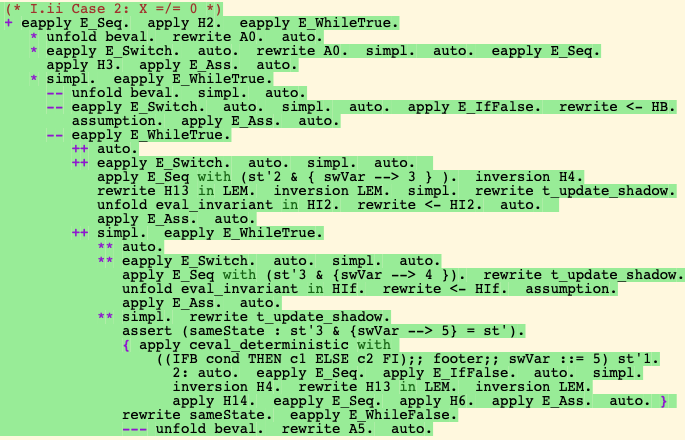
\includegraphics[scale=0.6]{alltrans_1_2}
        \caption{Coq proof of Theorem \ref{maintheo}, Case (I.ii).}
        \label{fig:maintheo12}
        \end{figure}
                
                The proof of this part is similar to Case (I.i), except that now the new hypothesis from \verb$destruct$ is instead
                \begin{verbatim}
LEM : beval st'1 cond = false\end{verbatim}
and so we proceed through the correspondingly different path of the while-switch construct.
            \end{itemize}
        \item[(II)] Transformed implies preprocessed.
        
            \noindent\begin{figure}[H]
        \centering
        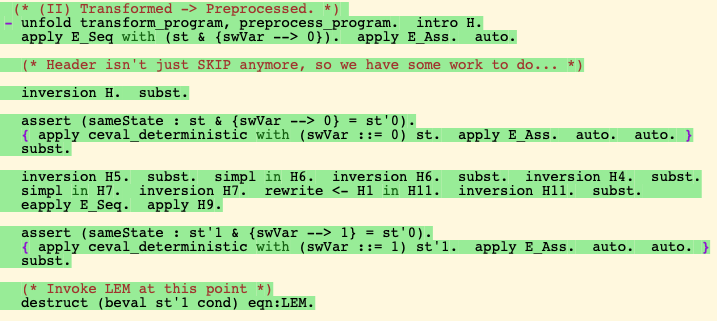
\includegraphics[scale=0.6]{alltrans_2}
        \caption{Coq proof of Theorem \ref{maintheo}, Case (II).}
        \label{fig:maintheo2}
        \end{figure}
            
            Similarly to Case (I), this part of the proof is setup work before we condition on the truth value of \verb$cond$ and split off into subcases.  The complete proof state at the end of this section is below.
\begin{verbatim}
header : com
cond : bexp
c1, c2, footer : com
HI1 : eval_invariant c1 swVar
HI2 : eval_invariant c2 swVar
HIf : eval_invariant footer swVar
HB : beval_invariant cond swVar
st, st' : state
H : (swVar ::= 0;;
     WHILE swVar <= 4
     DO SWITCH swVar
        [(0, header;; swVar ::= 1);
        (1,
        IFB cond THEN swVar ::= 2 ELSE swVar ::= 3 FI);
        (2, c1;; swVar ::= 4); (3, c2;; swVar ::= 4);
        (4, footer;; swVar ::= 5)] END) / st \\ st'
H5 : (WHILE swVar <= 4
      DO SWITCH swVar
         [(0, header;; swVar ::= 1);
         (1,
         IFB cond THEN swVar ::= 2 ELSE swVar ::= 3 FI);
         (2, c1;; swVar ::= 4); (3, c2;; swVar ::= 4);
         (4, footer;; swVar ::= 5)] END) /
     st & {swVar --> 0} \\ st'
H2 : (swVar ::= 0) / st \\ st & {swVar --> 0}
H3 : beval (st & {swVar --> 0}) (swVar <= 4) = true
st'1 : state
H8 : (WHILE swVar <= 4
      DO SWITCH swVar
         [(0, header;; swVar ::= 1);
         (1,
         IFB cond THEN swVar ::= 2 ELSE swVar ::= 3 FI);
         (2, c1;; swVar ::= 4); (3, c2;; swVar ::= 4);
         (4, footer;; swVar ::= 5)] END) /
     st'1 & {swVar --> 1} \\ st'
H4 : (SWITCH swVar
      [(0, header;; swVar ::= 1);
      (1, IFB cond THEN swVar ::= 2 ELSE swVar ::= 3 FI);
      (2, c1;; swVar ::= 4); (3, c2;; swVar ::= 4);
      (4, footer;; swVar ::= 5)]) / st & {swVar --> 0} \\
     st'1 & {swVar --> 1}
H7 : Some (header;; swVar ::= 1) =
     Some (header;; swVar ::= 1)
H11 : (header;; swVar ::= 1) / st & {swVar --> 0} \\
      st'1 & {swVar --> 1}
H9 : header / st & {swVar --> 0} \\ st'1
H13 : (swVar ::= 1) / st'1 \\ st'1 & {swVar --> 1}
LEM : beval st'1 cond = true
______________________________________(1/2)
((IFB cond THEN c1 ELSE c2 FI);; footer;; swVar ::= 5) /
st'1 \\ st'
______________________________________(2/2)
((IFB cond THEN c1 ELSE c2 FI);; footer;; swVar ::= 5) /
st'1 \\ st'\end{verbatim}
            \begin{itemize}
                \item[(II.i)] Case 1: Transformed implies preprocessed; boolean condition is true.
                
                \noindent\begin{figure}[H]
        \centering
        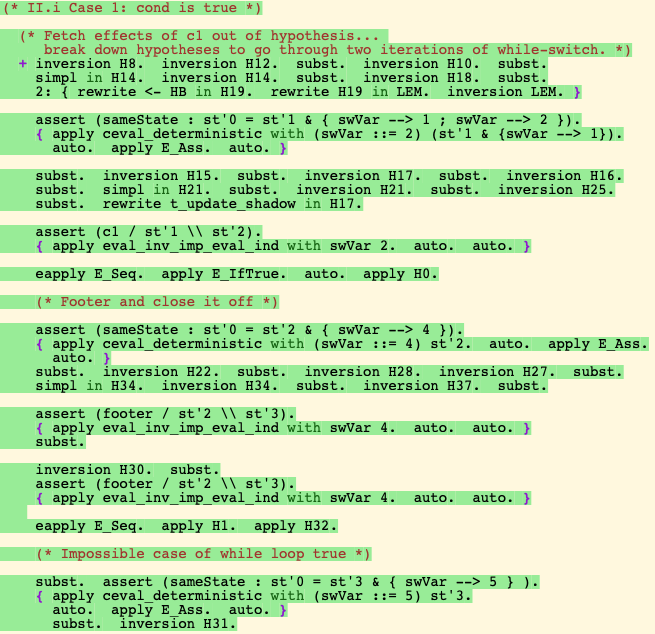
\includegraphics[scale=0.6]{alltrans_2_1}
        \caption{Coq proof of Theorem \ref{maintheo}, Case (II.i).}
        \label{fig:maintheo21}
        \end{figure}
                
                This subcase now runs through the (preprocessed) original program, with
                \begin{verbatim}LEM : beval st'1 cond = true.\end{verbatim}
                The details involve no new tactics, lemmas (save for invoking the assumption of boolean invariance rather than evaluation invariance), or bright ideas not seen in Case (I) and its subcases.
                
                \item[(II.ii)] Case 2: Transformed implies preprocessed; boolean condition is false.
                
                \noindent\begin{figure}[H]
        \centering
        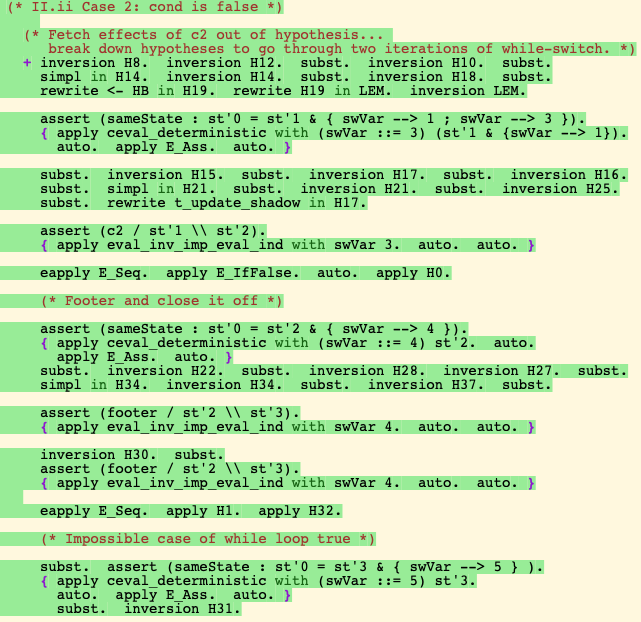
\includegraphics[scale=0.6]{alltrans_2_2}
        \caption{Coq proof of Theorem \ref{maintheo} Case (II.ii).}
        \label{fig:maintheo22}
        \end{figure}
                
                This subcase now runs through the (preprocessed) original program, with
                \begin{verbatim}LEM : beval st'1 cond = false.\end{verbatim}
                Finishing this subcase also completes the proof.  The final \verb$Qed$ of the code is omitted in the screenshot, which is several levels of indentation left of the above.\qedhere
            \end{itemize}
    \end{itemize}
\end{proof}
\end{theo}

\begin{rem}
    An alternate way to formulate the theorem of this section is, rather than demand a particular variable is not used, to instead write a function to generate a \emph{fresh variable} that does not prior exist in the program to be transformed.  We simply chose to explore a different direction; doing it that way and proving properties about such a function is not inherently difficult per se, but can be rather long and tedious. 
\end{rem}

\section{Flattening a While-Do-End construct}\label{4.4}
For the remainder of this chapter, we switch gears and study (as well as formalize) an example of dismantling and then flattening a While-Do-End construct described in \cite{Wang}, from where the diagrams below are taken.  Note that no general flattening algorithm is defined therein, simply an example given, and it is this example that we will formalize.  Other sources, such as \cite{CoNa}, dub this process \define{chenxification}, after the paper's author, Chenxi Wang.

\par This paper argues that determining the basic flow graph of a program is a straightforward operation when branch instructions and targets are easily discovered, and that it is a linear operation of complexity $O(n)$, where $n$ is the number of \define{basic blocks} in the program.  A basic block, essentially, is when one treats an entire block of a code as a first-class citizen\footnote{To make an analogy, consider how in Java everything is a class.  This is like saying an entire block of code is a class, and is itself the object of interest.}, as one can see in the figures labelled 2(b) and 3 below.  We'll make more precise what this means for us in the next section.
\par The idea is that (unobfuscated) real-world programs tend to have easily discernable control flow, which is encouraged for program clarity and readability, but this unfortunately also goes the other way in the event of an attacker gaining access to (some form of) the code, especially one conducting \define{static analysis}.  Thus, sensitive software should be developed in a clear manner, but obfuscated at the last step before it is pushed to production.

\noindent\begin{figure}[H]
        \centering
        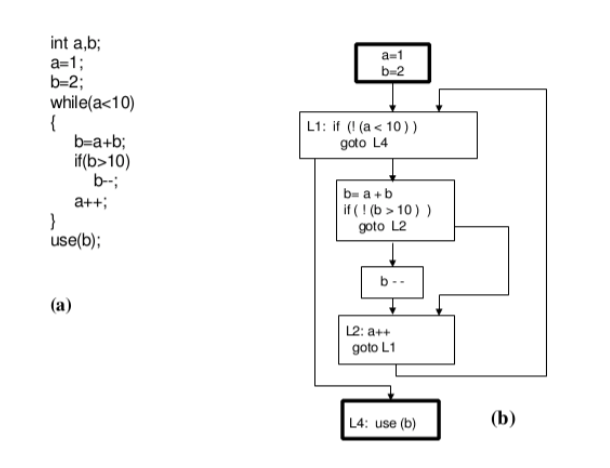
\includegraphics[scale=0.6]{WhileSmash.png}
        \caption{Dismantling While constructs, taken from \cite{Wang}.}
        \label{fig:chenxi}
        \end{figure}

The program in Figure \ref{fig:chenxi}(a) above is the original program in this example, written as a high-level construct in the familiar syntax of a typical imperative language.  It has a while loop with an if-then statement inside it.  
\par On the right in Figure \ref{fig:chenxi}(b), it is \define{dismantled} into a number of basic blocks, essentially replacing the While-Do-End construct with conditional GoTo statements at the end of some blocks.  The targets of these GoTos are determined dynamically with conditions on some variable in memory, instead of a direct (constant) address as the jump target.  We call the transformation from \ref{fig:chenxi}(a) to \ref{fig:chenxi}(b) \define{dismantling}.
\par The next level of the transformation is reminiscent of the transformation studied in the first half of this chapter, wherein these GoTos are replaced by entry into a switch statement.  In keeping consistent with prior terminology, Figure \ref{fig:chenxi2} below will be called flattening.  We'll develop a different language in the next section, however, and model this a bit differently from the switch statements of Sections \ref{4.2} and \ref{4.3}, as we are going to consider each boxed-in section of code in the diagram as its own basic block.

\noindent\begin{figure}[H]
        \centering
        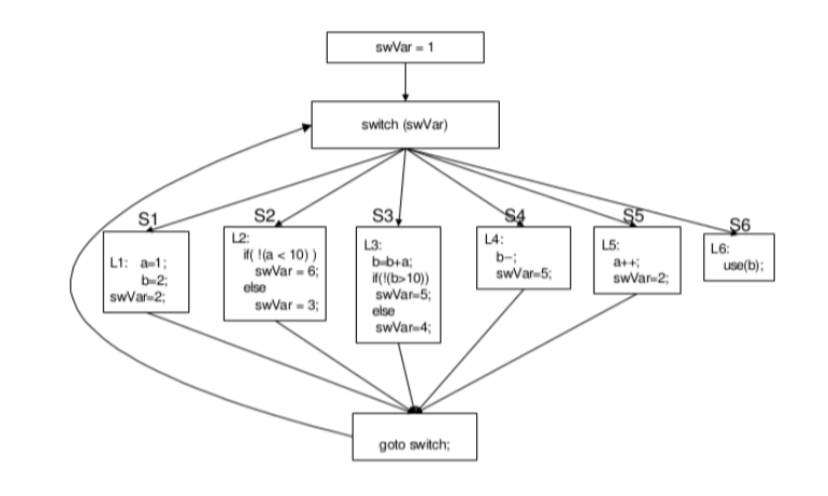
\includegraphics[scale=0.6]{WhileSmash2.png}
        \caption{Transforming While constructs, taken from \cite{Wang}.}
        \label{fig:chenxi2}
        \end{figure}

\section{Wrapping IMP in a flowchart language (IMP+Flow)}\index{IMP+Flow}

In this section, we describe a new lower-level formal language which will be used to represent the example from the previous section.  We'll call this language \emph{IMP+Flow}, short for flowchart.  The code for this and the following section can be found in the file \verb$OBFS_ImpFlow$ in the GitHub repository \cite{repo}.

\par This language is similar to intermediate languages that are transpiled to and used in the actual Cloakware obfuscation tool.  While very cumbersome to actually write programs in, it is well-suited to control flow flattening algorithms due to its treatment of basic blocks (of code) as first-class citizens.

\par Note here that the underlying program is the original IMP, and not the IMP+Switch defined in Section \ref{4.2}.  We handle switch statements differently here, by defining them as a type of block.

\begin{defin}[Command block, block dictionary]\index{block dictionary}
In Coq, we'll model the idea of a basic block as a \define{command block}.  This is essentially a wrapper type that takes an IMP command, together with information about what should happen after the command is executed.  Also, a \define{block dictionary} is a total map for command blocks (recall that this means it's a function from strings to command blocks).

\begin{verbatim}
Inductive comBlock : Type :=
  | bJump : com -> string -> comBlock
  | bConditional : com -> bexp -> string -> string -> comBlock
  | bSwitch : com -> string -> (nat -> string) -> comBlock
  | bEnd : com -> comBlock.

Definition blockDict : Type := total_map comBlock.
\end{verbatim}
\end{defin}

\par As seen above, there are four possibilities.  We describe them informally first, and follow with the formal definition in Coq of block evaluation.  The block could be a Jump (unconditional), where the next block is denoted by a string (to be used to index into a command dictionary for the next block).  It could be a Conditional (jump), which takes a boolean expression and two strings; the first of which is the index in the event that it is true and the second of which is the index for the event that it is false.  It could be a Switch (jump), which takes its first string argument as a switching variable, and then a map from $\N$ to strings which maps values taken on by the switching variable as a pointer into a command dictionary.  Finally, it can be an End (terminal) block, which signifies that the program's execution is finished. 

\begin{defin}[Block evaluation]\index{block evaluation}
The evaluation of a single basic block, along with shorthand notation, is defined inductively as follows.  The idea is that a complete IMP+Flow program will be equipped with a block dictionary that maps a string to each block that comprises it, like a label, and this will be passed as an argument to the relation defined below that evaluates just a single block.
\begin{verbatim}
Inductive blockEval : comBlock -> blockDict -> state -> state -> 
  option comBlock -> Prop :=
  | BE_Jump : forall c blockD st st' next nextBlock,
                ceval c st st' ->
                (blockD next) = nextBlock ->
                (blockEval (bJump c next) blockD st st' (Some nextBlock))
  | BE_CondTrue : forall c blockD st st' condition nextIf nextBlock nextElse,
                    ceval c st st' ->
                    (blockD nextIf = nextBlock) ->
                    (beval st' condition) = true ->
                    (blockEval (bConditional c condition nextIf nextElse) 
                     blockD st st' (Some nextBlock))
  | BE_CondFalse : forall c blockD st st' condition nextIf nextBlock nextElse,
                     ceval c st st' ->
                     (blockD nextElse = nextBlock) ->
                     (beval st' condition) = false ->
                     (blockEval (bConditional c condition nextIf nextElse) 
                      blockD st st' (Some nextBlock))
  | BE_Switch : forall c blockD st st' swVar swMap n nextPos nextBlock,
                  ceval c st st' ->
                  aeval st' (AId swVar) = n ->
                  swMap n = nextPos ->
                  blockD nextPos = nextBlock ->
                  (blockEval (bSwitch c swVar swMap) blockD st st' 
                   (Some nextBlock))
  | BE_End : forall c blockD st st',
               ceval c st st' ->
               (blockEval (bEnd c) blockD st st' None).

Notation "cmd '<<' blockD '/' st '\' stt '-->' nxt" :=
  (blockEval cmd blockD st stt nxt)
                  (at level 40, st at level 39).
\end{verbatim}
\end{defin}

\begin{defin}[Program (of blocks) evaluation]\index{program (of blocks) evaluation}
The evaluation of an entire program of blocks, along with shorthand notation, is defined inductively as follows.  Here, the command block argument represents the initial block (the start of the program), and its corresponding block dictionary.  
\par A program's execution is a valid relation (i.e.\ the program terminates) if and only if there is a reachable End block, which invokes the \verb$PE_Terminal$ rule below. There then needs to exist a valid sequence of \verb$PE_AddBlock$ invocations that can build this up one block at a time from the beginning of the program to that End block.
\begin{verbatim}
Inductive progEval : comBlock -> blockDict -> state -> state -> Prop :=
  | PE_Terminal : forall c blockD st st',
                     (blockEval (bEnd c) blockD st st' None) ->
                     progEval (bEnd c) blockD st st'
  | PE_AddBlock : forall newBlock currentChain blockD st st' st'',
                     (progEval currentChain blockD st'' st') ->
                     (blockEval newBlock blockD st st'' (Some currentChain)) ->
                     (progEval newBlock blockD st st').

Notation "cmd '<<' blockD '/' st '\\\' stt" :=
  (progEval cmd blockD st stt)
                  (at level 40, st at level 39).
\end{verbatim}
\end{defin}

\begin{defin}[IMP+Flow program and evaluation]\index{command evaluation!with flowchart}
Finally, for high-level usability, we'll put the pieces together and define the following.  An IMP+Flow program is formally defined as a pair, consisting of string (label) pointing to the starting block together with a block dictionary that contains a mapping from labels to all the command blocks that form the program.  The evaluation of an entire IMP+Flow program, then, uses the \verb$progEval$ previously defined, taking this starting block pointer and block dictionary as its arguments.
\begin{verbatim}
Definition IFP : Type := string * blockDict.

Definition IFPEval (program : IFP) st st' := 
  progEval ((snd program) (fst program)) (snd program) st st'.

Notation "prog '/' st '\\\' stt" :=
  (IFPEval prog st stt)
                  (at level 40, st at level 39).
\end{verbatim}
Here, \verb$string * blockDict$ denotes a product type, whilst \verb$fst$ and \verb$snd$ are the first and second projection functions, respectively.  
\end{defin}

\section{Flattening While-Do-End in IMP+Flow}

We'll now formalize the example from Section \ref{4.4}, albeit with some smaller numbers to make the execution proofs shorter, and since $use(b)$ from the diagrams there are not actually defined in the original paper, we'll instead take the product $a \times b$ (noted in Coq below as \verb$A * B$), and store it as a variable $RETURN$ as the final statement.

\par First, we define the blank block dictionary as the total map that sends everything to the terminal block containing just the \verb$SKIP$ command.  This is analogous to defining a blank map of natural numbers as sending every string to 0.

\begin{verbatim}
Definition Blank : blockDict := { --> (bEnd SKIP) }.
\end{verbatim}

The proofs in this section do not contain any inherently new tactics, beyond simply applying the new rules we have defined as required.

\begin{defin}
    We define the original program, our version of Figure 2(a) from Section \ref{4.4}, as this IMP program.
    
    \begin{verbatim}
Definition OriginalCommand : com :=
  WHILE (A <= 2) DO
    B ::= A + B ;;
    IFB (!(B <= 4)) THEN
      B ::= B - 1
    ELSE SKIP FI ;;
    A ::= A + 1
  END ;;
  RETURN ::= A * B.\end{verbatim}
    
    To (trivially) wrap up this single basic block as an IMP+Flow program requires the definition of a single terminal block with this command, a command dictionary that gives a name to this block, and then the final program which is a pair consisting of the starting block and the dictionary.
    
    \begin{verbatim}
Definition Main : comBlock :=
  bEnd OriginalCommand.

Definition OriginalDict : blockDict :=
  Blank & { "Main" --> Main }.

Definition OriginalProgram : IFP :=
  ("Main", OriginalDict).\end{verbatim}
\end{defin}

\begin{example}\label{while1}
The \verb$OriginalProgram$ will evaluate a state that begins with $A=1$ and $B=2$ to a final state that has $RETURN=12$.
\begin{proof}
    \noindent
    \begin{figure}[H]
        \centering
        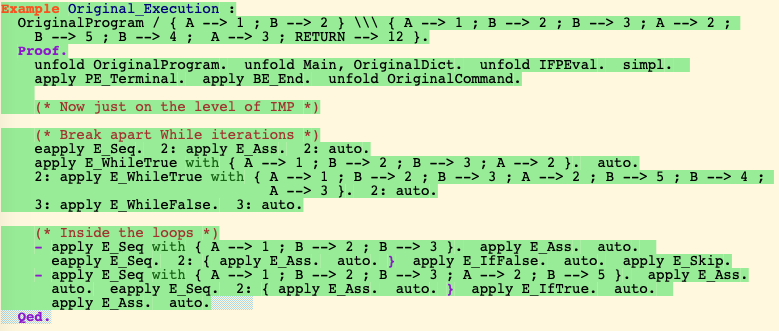
\includegraphics[scale=0.6]{while1.png}
        \caption{Proof in Coq of Example \ref{while1}.}
        \label{fig:while1}
        \end{figure}
\end{proof}
\end{example}

\begin{defin}
We now define the dismantled program, our version of Figure 2(b) from Section \ref{4.4}.  First, the underlying IMP programs are as follows.

\begin{verbatim}
Definition L1Com : com := SKIP.
Definition L2Com : com := A ::= A + 1.
Definition L3Com : com := B ::= A + B.
Definition L4Com : com := RETURN ::= A * B.
Definition L5Com : com := B ::= B - 1.\end{verbatim}
Next, these are wrapped up into command blocks, which declare the type of block along with the necessary arguments for what the next block should be.
\begin{verbatim}
Definition L1Blk : comBlock :=
  bConditional L1Com (!(A <= 2)) "L4" "L3".

Definition L2Blk : comBlock :=
  bJump L2Com "L1".

Definition L3Blk : comBlock :=
  bConditional L3Com (B <= 4) "L2" "L5".

Definition L4Blk : comBlock :=
  bEnd L4Com.

Definition L5Blk : comBlock :=
  bJump L5Com "L2".\end{verbatim}
 
Finally, we have the block dictionary that gives labels to each block, and the final dismantled program consisting of the starting block and the dictionary.
\begin{verbatim}
Definition DismantledDict : blockDict :=
  Blank & { "L1" --> L1Blk ; "L2" --> L2Blk ; "L3" --> L3Blk ; 
            "L4" --> L4Blk ; "L5" --> L5Blk }.

Definition DismantledProgram : IFP := ("L1", DismantledDict).
\end{verbatim}
\end{defin}

\begin{example}\label{while2}
The \verb$DismantledProgram$ will, like the \verb$OriginalProgram$, evaluate a state that begins with $A=1$ and $B=2$ to a final state that has $RETURN=12$.
\begin{proof}\ \newline
    \noindent
        \begin{figure}[H]
        \centering
        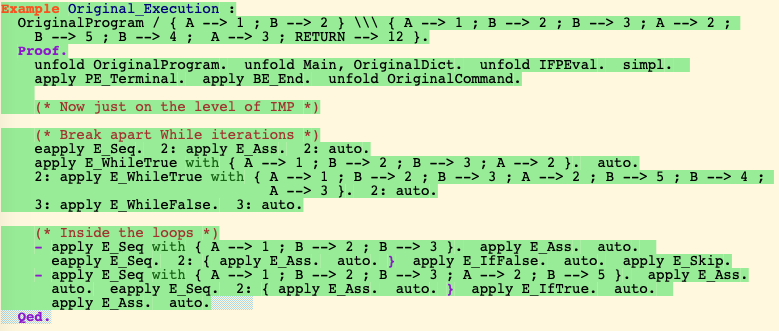
\includegraphics[scale=0.6]{while1.png}
        \caption{Proof in Coq of Example \ref{while2}.}
        \label{fig:while2}
        \end{figure}\qedhere
\end{proof}
\end{example}

\begin{defin}
We now define the flattened program, our version of Figure 3 from Section \ref{4.4}.  First, the underlying IMP programs are as follows.  Note the underlying program for what will be the switch block is just \verb$SKIP$, as the switching instruction is built into the block type and is no longer handled on the level of IMP.
\begin{verbatim}
Definition InitCom : com := SWITCH ::= 1.  

Definition SwitchCom : com := SKIP.

Definition S1Com : com :=
  IFB (A <= 2) THEN
    SWITCH ::= 2
  ELSE
    SWITCH ::= 5
  FI.

Definition S2Com : com :=
  B ::= B + A ;;
  IFB (B <= 4) THEN
    SWITCH ::= 4
  ELSE
    SWITCH ::= 3
  FI.

Definition S3Com : com :=
  B ::= B - 1 ;;
  SWITCH ::= 4.

Definition S4Com : com :=
  A ::= A + 1 ;;
  SWITCH ::= 1.

Definition S5Com : com :=
  RETURN ::= A * B.\end{verbatim}

We also need a \verb$SwitchMap$ that maps natural numbers (values that the switching variable could have), to labels that will index into the command dictionary.
\begin{verbatim}
Definition SwitchMap (n : nat) : string :=
  match n with
  | 1 => "S1"
  | 2 => "S2"
  | 3 => "S3"
  | 4 => "S4"
  | 5 => "S5"
  | 6 => "S6"
  | _ => ""
\end{verbatim}
Next, we wrap up the IMP programs into command blocks.
\begin{verbatim}
Definition InitBlk : comBlock :=
  bJump InitCom "Switch".

Definition SwitchBlk : comBlock :=
  bSwitch SwitchCom SWITCH SwitchMap.

Definition S1Blk : comBlock :=
  bJump S1Com "Switch".

Definition S2Blk : comBlock :=
  bJump S2Com "Switch".

Definition S3Blk : comBlock :=
  bJump S3Com "Switch".

Definition S4Blk : comBlock :=
  bJump S4Com "Switch".

Definition S5Blk : comBlock :=
  bEnd S5Com.\end{verbatim}
And finally, the block dictionary and final program are as follows.
\begin{verbatim}
Definition FlattenedDict : blockDict :=
  Blank & { "Init" --> InitBlk ; "Switch" --> SwitchBlk ; "S1" --> S1Blk ; 
            "S2" --> S2Blk ; "S3" --> S3Blk ; "S4" --> S4Blk ; "S5" --> S5Blk }.

Definition FlattenedProgram : IFP := ("Init", FlattenedDict).
\end{verbatim}
\end{defin}
\begin{example}\label{while3b}
The \verb$FlattenedProgram$ will, like the \verb$OriginalProgram$ and the \verb$DismantledProgram$, evaluate a state that begins with $A=1$ and $B=2$ to a final state that has $RETURN=12$.
\begin{proof}\ \newline
    \noindent
    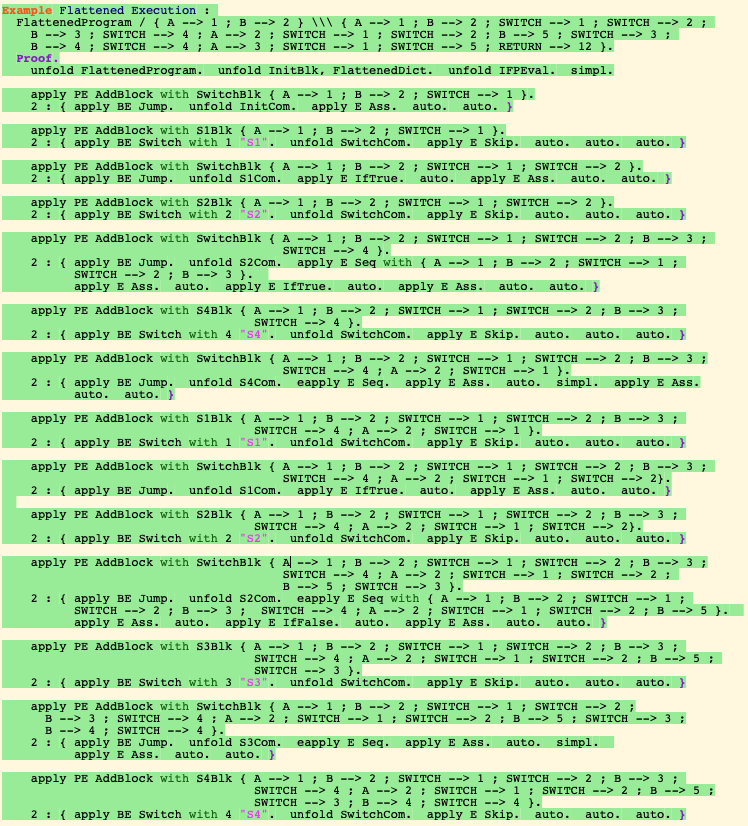
\includegraphics[scale=0.6]{while3a}
    \noindent
        \begin{figure}[H]
        \centering
        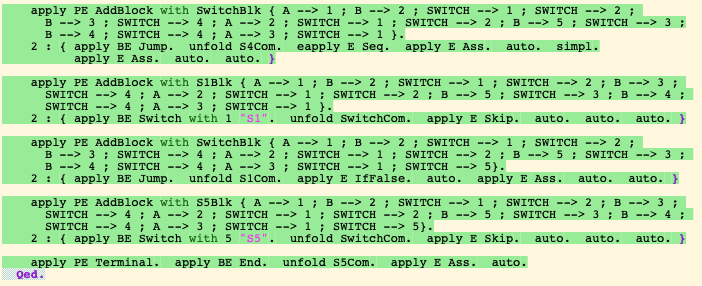
\includegraphics[scale=0.6]{while3b.png}
        \caption{Proof in Coq of Example \ref{while3b}.}
        \label{fig:while3b}
        \end{figure}
\end{proof}
\end{example}

Through this series of Coq examples, we have provided a formal proof for the correctness of the examples given in \cite{Wang}, as shown in Figures \ref{fig:chenxi} and \ref{fig:chenxi2}.

\begin{comment}
\section{Data obfuscation in IMP}
\section{Layout obfuscation in IMP}
\section{Control flow flattening in CompCert}
\section{Mixed boolean arithmetic in CompCert}
\end{comment}

\chapter{Epilogue}
\section{Summary}
Motivated by the Cloakware obfuscation tool produced at Irdeto and the mutual interests in formal verification of the present author and his supervisor there, Bahman Sistany, who was also a former student of Prof. Felty, we defined a project to use IMP in the Coq proof assistant to formally specify and prove correct some transformations, namely opaque predicates and control flow flattening of If-Then-Else constructs.
\par All of the transformations we studied fall under the category of control-flow altering obfuscating transformations.  We chose these over other kinds because they are non-trivial and interesting, but still quite doable for a project at this level.  One could, of course, always just add some pointless lines of code as an obfuscation (and certainly this can be useful in tandem with control-flow altering), but doing this in and of itself would not obfuscate the control-flow graph.  We note further that code obfuscation falls under the general category of program transformations --- compiling and transpiling --- but a key distinction is in the flavor.  That is, while usually a compiler is trying to \emph{optimize} code, we are in fact doing the opposite on purpose.

\par We ran into some issues with our first naive attempt to formalize opaque predicate transformations, and came up with an alternate assignment-free formulation to prove command equivalence, but also considered Hoare logic to look at specific pre- and post-conditions, which may be a more realistic approach in certain large real-world programs and transformations.
\par We specified and proved correct (in Coq) a version of control flow flattening, targeting a single If-Then-Else construct.  We came up with invariant conditions that implied the separation between the switching variable introduced by the transformation and the original program.
\par This work was presented at the end of the summer of 2018 at Irdeto, and garnered interest from developers, reverse engineers, and managers, who saw potential for the use of formal methods in the next generation of obfuscation tools, either in place of or in addition to the ad-hoc testing process currently used.
\par Additionally, we also investigated an example of the dismantling and flattening of a While-Do-End construct laid out in \cite{Wang}, and developed a lower-level flowchart language that wraps around IMP, which runs parallel to part of the real-world process of Cloakware's control flow flattening process.

\section{Related works}
There have been three papers, in all of which Sandrine Blazy (Universit\'{e} de Rennes 1) appears as a coauthor, that study code obfuscation in Coq.

\subsection*{Towards a formally verified obfuscating compiler}
\par \emph{Towards a formally verified obfuscating compiler} \cite{Blazy1} also uses IMP as the language for obfuscation, but studies \define{data obfuscation} techniques, as opposed to the \define{layout obfuscation} techniques which opaque predicates and control flow flattening fall under.  
\par The first particular transformation studied herein is \define{obfuscating integer constants}, wherein all integer values are substituted by different ones in a \define{distorted semantics} using an obfuscating function $O: \N \to \N$.  The other discussed is \define{variable encoding}, which changes the names of variables.  A real-life application of this could be, for instance, to change a descriptive variable name like $account\_balance$ to a string of gibberish.  
\par This is an inherently different class of techniques from the ones studied in the present work, and one can make a simple combinatorial argument that putting them together in the same obfuscation transformation would generate a synergistic effect on making a program more difficult to analyze.

\subsection*{Formal verification of control-flow graph flattening}
\par \emph{Formal verification of control-flow graph flattening} \cite{Blazy2} also studies control flow flattening, but the authors use the \define{CLight} language of CompCert (the formally verified C compiler in Coq, discussed in Chapter \ref{two}).  CLight is the first intermediate language in the CompCert compiler, and the strategy used was to prove the correctness of the obfuscation strictly there, from which CompCert's own proofs of semantic preservation give the correctness of the rest of the compilation process ``for free".
\par On the one hand, this makes the work less elementary and less accessible, as it works with a nontrivial subset of the real C language, but on the other it is clear evidence that formal verification of obfuscation techniques need not be restricted to a small language like IMP (which would never be used in real software development), and other real-world practicalities considered in this paper include simulation techniques and analysis of running time.  
\par This work also discusses some techniques for combining obfuscation techniques, such as splitting a switching variable into two different variables that are updated at different points of a program, as well as randomly encoding the values of the switch cases so that they are not just consecutive numbers beginning with 1.  These are necessary considerations, since we need to think one level higher about our attackers, and obfuscate the fact that we are obfuscating particular parts of our code with CFG flattening in the first place!
\par In comparing this work to ours, the present author believes there is merit both in the IMP and the CompCert routes.  In the former, the language used is of minimal complexity, which allows not only for specifications and proofs of transformations to be developed quicker without being bogged down in unnecessarily complicated features of the underlying language, but is also better suited for pedagogical purposes.  IMP is also Turing complete, so from a theoretical point of view there is no loss of generality in proofs made using it --- they can always be adapted to CompCert later.  But on the other hand, CompCert is, of course, closer to languages that would be of interest to real-world software development and so more practical in that sense.
\par The authors ran into a similar issue as in the present work of needing to separate switching variables from those in the program to be transformed, but their solution was different --- they instead use a function to parse the program to be transformed and generate a \define{fresh variable} which doesn't appear there to be used for the transformation.  From a practical point of view, this is perhaps more natural, and in line with how a real obfuscating tool would function --- generating new variables rather than demand that a certain specifically named variable doesn't exist in the source program.  Theoretically, though, these are equivalent, since any program can contain only finitely many variable names, and there are an infinite number to choose from. 

\subsection*{Formal verification of a program obfuscation based on mixed boolean-arithmetic expressions}
\par \emph{Formal verification of a program obfuscation based on mixed boolean-arithmetic expressions} \cite{Blazy3}\index{mixed boolean arithmetic} continues to work in CLight, which studies obfuscations that involve mixing arithmetic operators and bitwise boolean operators.  This is another data obfuscation which appears frequently in real-world binary code, but as it is based on features wildly beyond the capabilities of IMP, a detailed discussion is beyond the scope of the present work.

\section{Future directions}
The work done to date on formal verification of obfuscation, both in the present work and in the papers of Dr. Blazy et al., while providing a solid proof-of-concept that obfuscation tools of the future could support formal verification, are still limited in scope in the sense that they treat individual transformations.
\par A real world obfuscator mixes many different transformations together at once, often in non-deterministic ways for \define{diversification} of obfuscations, and so some form of compositionality would need to be implemented on these formal proofs to be able to use them together and preserve the desired formulation of correctness.  In principal, compositionality should be obvious if the formulations of correctness agree, but it simply has not yet been investigated by anyone we are aware of.  This is a natural next step towards bridging the gap between theory and practice, and in particular, the code developed here on opaque predicates and control flow flattening in IMP may be compatible in some way with the separate data obfuscations of \cite{Blazy1}.  We contacted the authors of this paper in hopes of being able to obtain the code, however we received a reply that it was unfortunately unavailable.

\par Formal verification promises a high assurance of correctness, but comes at a large price of time and manpower!  It is thus best suited in conditions where the particular code base to be verified is not overly complex, and where the safety is of critical importance.  We believe that code obfuscation indeed checks off both of these boxes, and hope to see a future where commercial tools for obfuscation, even if not completely formally verified, at least make some use of these techniques for their own ``street cred" in reliability and correctness.  That said, it can still in practice be challenging to convince members of industry who are not prior versed in formal methods that it is worth the resources necessary to tackle the extra complexity introduced by doing these proofs.

\par Furthermore, we (along with the three aforementioned pieces of related work) have, in the formal setting of Coq, only tackled one desired property of obfuscation --- correctness.  That is, 
some form of the semantics of the program, or relationship between inputs and outputs, should be preserved.  This is an important property --- perhaps the most fundamental, for if the result of an obfuscation is not even the same program anymore, then all else is moot.  But there are, of course, other properties that have not been touched upon, namely:
\begin{itemize}
\item The transformation should be \define{small} - the obfuscated program should be at most polynomially larger than the original.
\item The transformation should be \define{efficient} - the obfuscated program should be at most polynomially slower than the original.
\item A clear formulation of what it means for the obfuscating algorithm to actually do its job of hiding information.  In the most general sense, what is desired is a \define{virtual black box}, in which \define{source code access} (being able to read the code of the obfuscated program) should not give an attacker a higher probability of being able to compute some \define{asset} (that is, a property that we wish to hide) than \define{oracle access} (only being able to query the program with an input and receiving the corresponding output, but no other information whatsoever).
\end{itemize}
The first two conditions above are sanity checks that our obfuscating algorithms are not degenerate and output a feasible and usable program.  The final one is perhaps the most difficult to tackle.   In fact, the virtual black box property described is provably impossible in the general case.  
\par This impossibility result\index{impossibility result} can be proven by constructing a counterexample program \cite[Ch.5]{CoNa} which is like a Crackme (see Chapter \ref{intro}) with a secret key, along with an alternate mode of operation that divulges the key if it can recognize a program passed as a parameter to be equivalent to itself (i.e.\ a self-referential argument, remniscent of \define{G\"{o}del's Incompleteness Theorem} \cite[Ch.7]{vanDalen}).  For such a program, oracle access does no better than attempting to brute-force the key, yet it becomes trivial to break with source code access. 
\par Such a strong and absolute requirement, however, lies in the realms of the idealist and the theoretical, and is perhaps both impractical and unnecessary in the real world, so it would be better to come up with security goals that are ``good enough in practice", and then formalize and prove them correct, either for individual transformations, individual tools, or individual use cases.

\par A talk given by Blazy, \cite{BlazyTalk}, offers an interesting insight that may be a useful lead to this end.  Blazy raises the point that a proof serves not only as a guarantee of correctness, but may also be used to evaluate and compare obfuscation techniques.  Since the proofs reveal the steps required to reverse the effects of an obfuscation, they could potentially offer some measure to the difficulty of reverse engineering obfuscated code, as well as compare the potency of different obfuscation algorithms.  The actual details of how to do this do not yet seem to be clearly defined, but it certainly is an interesting direction to consider.

\par In closing, we stress, once more, that it \emph{is} important to actually apply formal specifications and methods to security goals and metrics in some form, so we can come full circle and give prospective clients of an obfuscation tool a clear answer to the \emph{other} big question ``How exactly will using this improve the security of my programs?" and be able to back our answer with a proof that it actually does so.


\begin{comment}
\chapter{Cryptographic obfuscation in IMP/Coq}
Tentative --- interesting future topic I haven't looked too much into yet.
\end{comment}

\phantomsection
\addcontentsline{toc}{chapter}{Index}
\printindex


\bibliographystyle{alpha}
\bibliography{tezos}
\addcontentsline{toc}{chapter}{Bibliography}
\nocite{HuRy}
%\nocite{R2}
%\nocite{SMTCoq}
\nocite{Wang}
%\nocite{Opaque}
%\nocite{Pier}
\nocite{Laszlo}
%\nocite{CoNa}
%\nocite{Coq}


\end{document}
